% Options for packages loaded elsewhere
\PassOptionsToPackage{unicode}{hyperref}
\PassOptionsToPackage{hyphens}{url}
%
\documentclass[
]{book}
\usepackage{amsmath,amssymb}
\usepackage{iftex}
\ifPDFTeX
  \usepackage[T1]{fontenc}
  \usepackage[utf8]{inputenc}
  \usepackage{textcomp} % provide euro and other symbols
\else % if luatex or xetex
  \usepackage{unicode-math} % this also loads fontspec
  \defaultfontfeatures{Scale=MatchLowercase}
  \defaultfontfeatures[\rmfamily]{Ligatures=TeX,Scale=1}
\fi
\usepackage{lmodern}
\ifPDFTeX\else
  % xetex/luatex font selection
\fi
% Use upquote if available, for straight quotes in verbatim environments
\IfFileExists{upquote.sty}{\usepackage{upquote}}{}
\IfFileExists{microtype.sty}{% use microtype if available
  \usepackage[]{microtype}
  \UseMicrotypeSet[protrusion]{basicmath} % disable protrusion for tt fonts
}{}
\makeatletter
\@ifundefined{KOMAClassName}{% if non-KOMA class
  \IfFileExists{parskip.sty}{%
    \usepackage{parskip}
  }{% else
    \setlength{\parindent}{0pt}
    \setlength{\parskip}{6pt plus 2pt minus 1pt}}
}{% if KOMA class
  \KOMAoptions{parskip=half}}
\makeatother
\usepackage{xcolor}
\usepackage{longtable,booktabs,array}
\usepackage{calc} % for calculating minipage widths
% Correct order of tables after \paragraph or \subparagraph
\usepackage{etoolbox}
\makeatletter
\patchcmd\longtable{\par}{\if@noskipsec\mbox{}\fi\par}{}{}
\makeatother
% Allow footnotes in longtable head/foot
\IfFileExists{footnotehyper.sty}{\usepackage{footnotehyper}}{\usepackage{footnote}}
\makesavenoteenv{longtable}
\usepackage{graphicx}
\makeatletter
\def\maxwidth{\ifdim\Gin@nat@width>\linewidth\linewidth\else\Gin@nat@width\fi}
\def\maxheight{\ifdim\Gin@nat@height>\textheight\textheight\else\Gin@nat@height\fi}
\makeatother
% Scale images if necessary, so that they will not overflow the page
% margins by default, and it is still possible to overwrite the defaults
% using explicit options in \includegraphics[width, height, ...]{}
\setkeys{Gin}{width=\maxwidth,height=\maxheight,keepaspectratio}
% Set default figure placement to htbp
\makeatletter
\def\fps@figure{htbp}
\makeatother
\setlength{\emergencystretch}{3em} % prevent overfull lines
\providecommand{\tightlist}{%
  \setlength{\itemsep}{0pt}\setlength{\parskip}{0pt}}
\setcounter{secnumdepth}{5}
\usepackage{booktabs}
\ifLuaTeX
  \usepackage{selnolig}  % disable illegal ligatures
\fi
\usepackage[]{natbib}
\bibliographystyle{plainnat}
\usepackage{bookmark}
\IfFileExists{xurl.sty}{\usepackage{xurl}}{} % add URL line breaks if available
\urlstyle{same}
\hypersetup{
  pdftitle={ADS - Tecnologia da Informação e Telecomunicações 2025 - Anotações de aula},
  pdfauthor={Professor Miguel Suez Xve Penteado},
  hidelinks,
  pdfcreator={LaTeX via pandoc}}

\title{ADS - Tecnologia da Informação e Telecomunicações 2025 - Anotações de aula}
\author{Professor Miguel Suez Xve Penteado}
\date{2025-03-22}

\begin{document}
\maketitle

{
\setcounter{tocdepth}{1}
\tableofcontents
}
\chapter*{Sobre estas anotações}\label{sobre-estas-anotauxe7uxf5es}
\addcontentsline{toc}{chapter}{Sobre estas anotações}

Estas anotações são apenas lembretes das aulas expostas em sala, durante a disciplina de ENGENHARIA DE SOFTWARE.

\subsection{ACESSO Anotações de aula no ceular (github)}\label{acesso-anotauxe7uxf5es-de-aula-no-ceular-github}

\url{https://miguel7penteado.github.io/ADS-TecnologiaInformacaoComunicacoes2025/}

\includegraphics{images/qr-code/repositório.jpg}

\subsection{Anotações de aula: Suporte para Celulares}\label{anotauxe7uxf5es-de-aula-suporte-para-celulares}

No celular o conteúdo pode ser lido no formato EPUB, sendo sugerio os seguintes aplicativos:

\subsection{\texorpdfstring{\textbf{Moon+ Reader (Google Play - loja de aplicativos oficial do google)}}{Moon+ Reader (Google Play - loja de aplicativos oficial do google)}}\label{moon-reader-google-play---loja-de-aplicativos-oficial-do-google}

\url{https://play.google.com/store/apps/details?id=com.flyersoft.moonreader&pcampaignid=web_share}


\includegraphics{images/qr-code/leitor_ebook/MoonReaderPlus.jpg}

\subsection{\texorpdfstring{\textbf{Epub Reader (AppStore - loja de aplicativos oficial da Apple)}}{Epub Reader (AppStore - loja de aplicativos oficial da Apple)}}\label{epub-reader-appstore---loja-de-aplicativos-oficial-da-apple}

\url{https://apps.apple.com/br/app/epub-leitor-ler-epub-chm-txt/id1296870631?platform=iphone}


\includegraphics{images/qr-code/leitor_ebook/AppleEpubReader.jpg}

\chapter*{INTRODUÇÃO DA DISCIPLINA}\label{introduuxe7uxe3o-da-disciplina}
\addcontentsline{toc}{chapter}{INTRODUÇÃO DA DISCIPLINA}

coming soon

\section{Livros-Texto da disciplina}\label{livros-texto-da-disciplina}

\subsection{Bibliografia Básica}\label{bibliografia-buxe1sica}

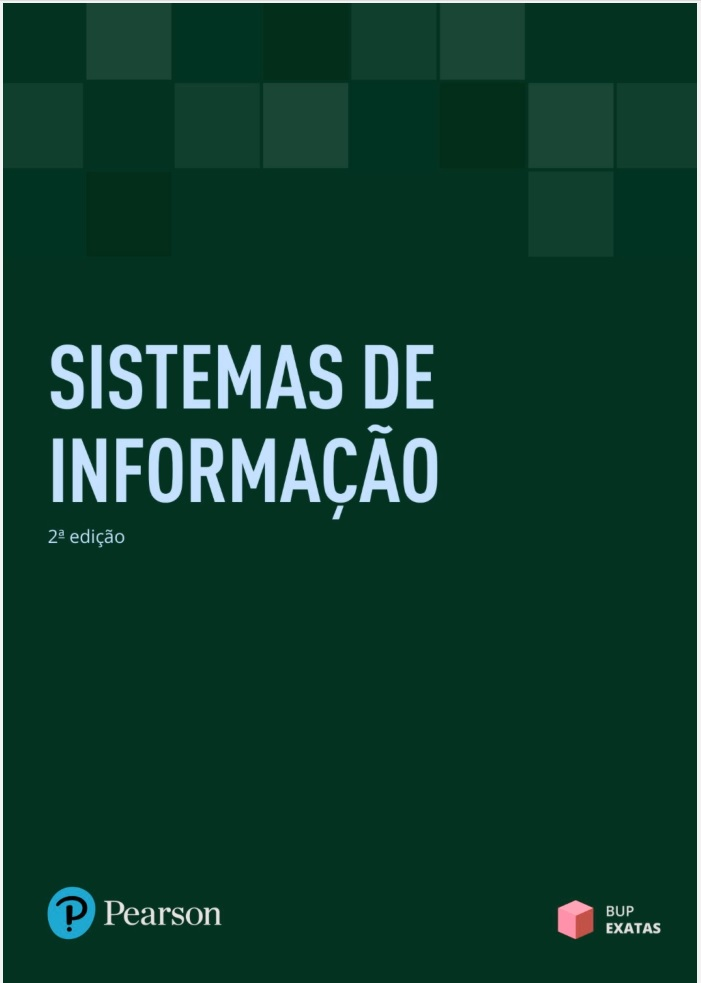
\includegraphics[width=3.03125in,height=\textheight]{images/livros/livro-SistemasDeInformação-BelmiroNascimentoJoao-2ed-person.jpg}

( JOÃO, Belmiro N. Sistemas de Informação - São Paulo: Pearson Education do Brasil, 2019.)

JOÃO, Belmiro N. Informática Aplicada. São Paulo: Pearson Education do Brasil, 2019.

GONÇALVES, G. R. B. Sistemas de informação. Porto Alegre: SAGAH, 2017.

SILVA, K. C. N.; BARBOSA, C.; CÓRDOVA JUNIOR, R. S. Sistemas de informações gerenciais. Porto Alegre: SAGAH, 2018.

\subsection{Bibliografia Complementar}\label{bibliografia-complementar}

LAUDON, Kenneth C; LAUDON, Jane P. Sistemas de Informação Gerenciais. São Paulo: Pearson Education do Brasil, 2014.

MUNHOZ, Antônio S. Fundamentos de Tecnologia da Informação e análise de sistemas para não analistas. Curitiba: Intersaberes, 2017.

MARÇULA, M.; BENINI FILHO, P. A. Informática: Conceitos e Aplicações. 5.Ed. São Paulo: Erica: 2019.

RAINER JUNIOR, R. K.; CEGIELSKI, C. G. Introdução a sistemas de informação. - 5. ed.~- Rio de Janeiro: Elsevier, 2016.

STAIR, Ralph M; REYNOLDS, George W. Princípios de sistemas de informação / Ralph M. Stair. São Paulo: Cengage Learning, 2015.

\section{CALENDÁRIO DE AULAS E PROVAS}\label{calenduxe1rio-de-aulas-e-provas}

\textbf{Fevereiro 2025}

\begin{longtable}[]{@{}cccc@{}}
\toprule\noalign{}
No. & fevereiro 2025 & Semana & conteúdo \\
\midrule\noalign{}
\endhead
\bottomrule\noalign{}
\endlastfoot
01 & 17/02/2025 & Segunda-feira & Inaugural \\
02 & 24/02/2025 & Segunda-feira & Aula 01 \\
\end{longtable}

\textbf{Março 2025}

\begin{longtable}[]{@{}cccc@{}}
\toprule\noalign{}
No. & Março 2025 & Semana & conteúdo \\
\midrule\noalign{}
\endhead
\bottomrule\noalign{}
\endlastfoot
03 & 03/03/2025 & Segunda-feira & Feriado \\
04 & 10/03/2025 & Segunda-feira & Aula 02 \\
05 & 17/03/2025 & Segunda-feira & Aula 03 \\
06 & 24/03/2025 & Segunda-feira & Aula 04 \\
07 & 31/03/2025 & Segunda-feira & NP1 \\
\end{longtable}

\textbf{Abril 2025}

\begin{longtable}[]{@{}cccc@{}}
\toprule\noalign{}
No. & Abril 2025 & Semana & conteúdo \\
\midrule\noalign{}
\endhead
\bottomrule\noalign{}
\endlastfoot
08 & 07/04/2025 & Segunda-feira & Aula 05 \\
09 & 14/04/2025 & Segunda-feira & Aula 06 \\
10 & 21/04/2025 & Segunda-feira & Aula 07 \\
11 & 28/04/2025 & Segunda-feira & Aula 08 \\
\end{longtable}

\textbf{maio 2025}

\begin{longtable}[]{@{}cccc@{}}
\toprule\noalign{}
No. & Maio 2025 & Semana & conteúdo \\
\midrule\noalign{}
\endhead
\bottomrule\noalign{}
\endlastfoot
12 & 05/05/2025 & Segunda-feira & Aula 09 \\
13 & 12/05/2025 & Segunda-feira & Aula 10 \\
14 & 19/05/2025 & Segunda-feira & NP2 \\
15 & 26/05/2025 & Segunda-feira & SUB \\
\end{longtable}

\textbf{junho 2025}

\begin{longtable}[]{@{}cccc@{}}
\toprule\noalign{}
No. & Junho 2025 & Semana & conteúdo \\
\midrule\noalign{}
\endhead
\bottomrule\noalign{}
\endlastfoot
12 & 02/06/2025 & Segunda-feira & PLANTÃO \\
13 & 09/06/2025 & Segunda-feira & PLANTÃO \\
14 & 16/06/2025 & Segunda-feira & EXAME \\
15 & 23/06/2025 & Segunda-feira & VISTAS \\
\end{longtable}

\chapter{INTRODUÇÃO A TIC (TECNOLOGIA DA INFORMAÇÃO E COMUNICAÇÕES)}\label{introduuxe7uxe3o-a-tic-tecnologia-da-informauxe7uxe3o-e-comunicauxe7uxf5es}

\section{Conceitos de Sistemas de Informação}\label{conceitos-de-sistemas-de-informauxe7uxe3o}

\subsection{O Dado}\label{o-dado}

Conceito de Dados (DATA) segundo Prof \textbf{Belmiro Nascimento João - USP - (autor SISTEMAS DA INFORMAÇÃO - 2a edição 2017)}

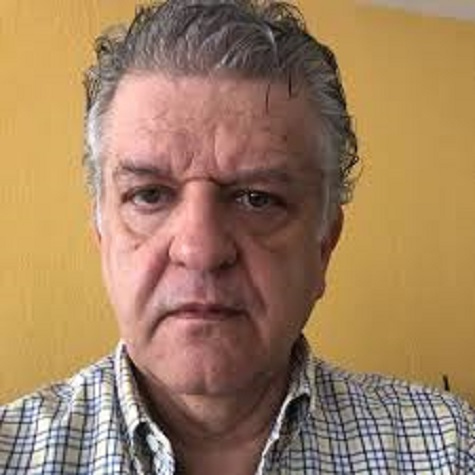
\includegraphics[width=1.36458in,height=\textheight]{images/belmiro_do_nascimento_joao-2.jpg}

\begin{quote}
\textbf{Dados} \emph{são sequências de fatos ainda não analisados, antes de serem organizados e ar­ ranjados de um jeito que as pessoas possam compreendê-los.} (João, Belmiro Nascimento - 2017)
\end{quote}

\begin{quote}
\textbf{Informação} \emph{é um dado organizado e apresentado de forma útil.} (João, Belmiro Nascimento - 2017)
\end{quote}

\begin{quote}
\textbf{Conhecimento} é o resultado da aplicação da informação para tomada de decisão. (João, Belmiro Nascimento - 2017)
\end{quote}

Exemplo de \textbf{Dados} versus \textbf{Informação}:

As caixas dos supermercados registram milhões de dados, como o código de barras dos produtos. Se somarmos e analisarmos esses dados, pode­ mos obter informações significativas, como o número total de detergentes vendidos em uma loja ou as vendas por região.

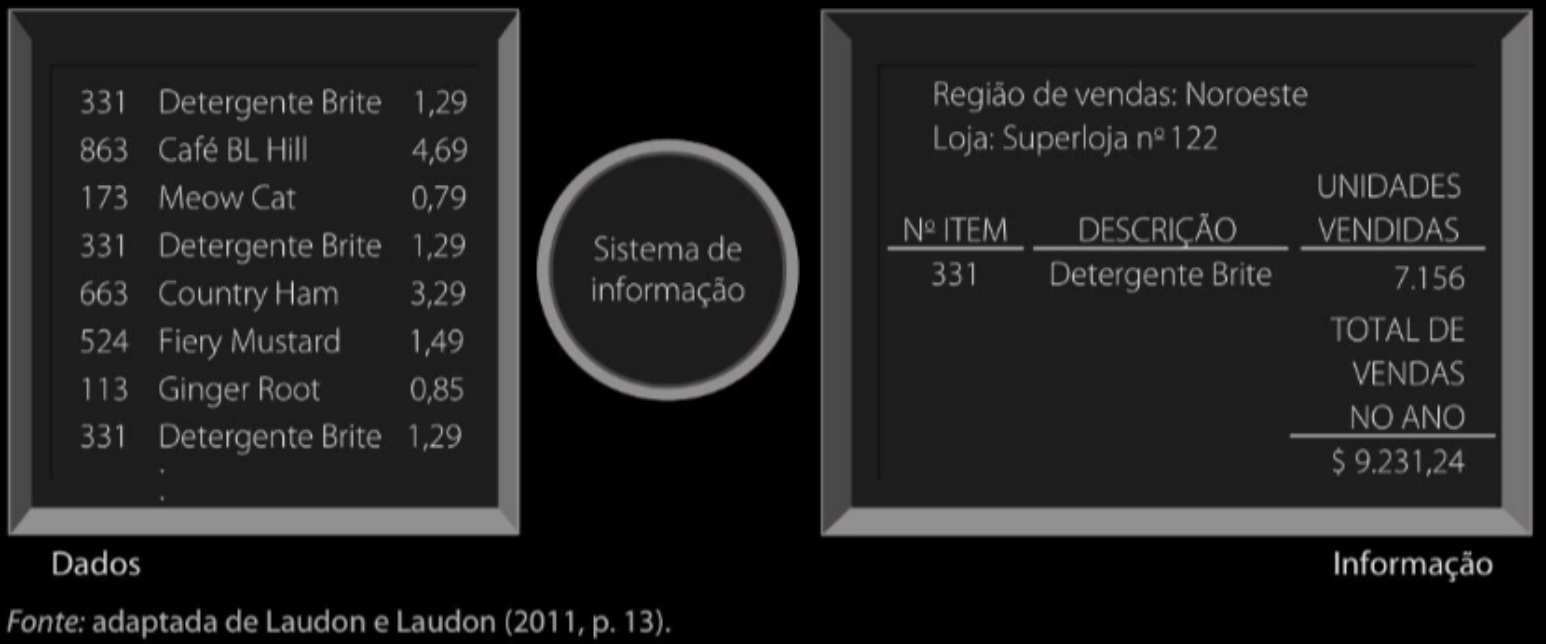
\includegraphics{images/1-dados-info/Dados-Info.jpg}

Fonte: LAUDON E LAUDON (2011, Pág 13)

\subsubsection{\texorpdfstring{Conceito de TIC -Tecnologia da informação e Comunicação \textbf{segundo} \emph{Kenneth C. LAUDON, Jane P. LAUDON} (2011)}{Conceito de TIC -Tecnologia da informação e Comunicação segundo Kenneth C. LAUDON, Jane P. LAUDON (2011)}}\label{conceito-de-tic--tecnologia-da-informauxe7uxe3o-e-comunicauxe7uxe3o-segundo-kenneth-c.-laudon-jane-p.-laudon-2011}

\begin{quote}
As \textbf{Tecnologias da Informação e Comunicação} (TICs) são um \textbf{CONJUNTO de tecnologias} que combinam:

\textbf{Tecnologia da Informação (TI)}: Refere-se ao hardware, software e redes necessários para processar, armazenar e distribuir dados e informações;

\textbf{Tecnologia da Comunicação}: Inclui as tecnologias que facilitam a comunicação e o compartilhamento de informações, como redes de telecomunicações, internet e dispositivos móveis.
\end{quote}

\subsubsection{\texorpdfstring{Conceito de Sistemas de Informação (SI) segundo \emph{Kenneth C. LAUDON, Jane P. LAUDON} (2011)}{Conceito de Sistemas de Informação (SI) segundo Kenneth C. LAUDON, Jane P. LAUDON (2011)}}\label{conceito-de-sistemas-de-informauxe7uxe3o-si-segundo-kenneth-c.-laudon-jane-p.-laudon-2011}

\begin{figure}
\centering
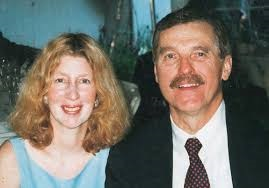
\includegraphics{images/Ken_Jane.jpg}
\caption{Prof Ken C. Laudon (1944 - 2019) e Jane Price Laudon - Universidade Columbia}
\end{figure}

\begin{quote}
\emph{``Tecnicamente, um \textbf{sistema de informação (Si)} é um CONJUNTO DE COMPONENTES RELACIONADOS entre si que COLETAM (ou recuperam), PROCESSAM, ARMAZENAM c DISTRIBUEM {[}o que ?{]} INFORMAÇÕES que servem para apoiar a TOMADA DE DECISÕES, a COORDENAÇÃO e o CONTROLE de uma organização.'' (LAUDON; LAUDON, 2011)}
\end{quote}

PERGUNTA: \emph{Um \textbf{SISTEMA DE INFORMAÇÃO (SI)} é a mesma coisa que um \textbf{computador (smartphone) com um software (app)}}?

a ) sim ? Porque ?\_\_\_\_\_\_\_\_\_\_\_\_\_\_\_\_\_\_\_\_\_\_\_\_\_\_\_\_\_\_\_\_\_\_\_\_\_\_\_\_\_\_\_\_\_\_\_\_\_\_\_\_\_\_\_\_\_\_\_\_\_\_\_\_\_\_\_\_\_\_\_\_\_\_\_\_\_\_\_\_\_\_\_\_\_\_\_\_\_

\begin{enumerate}
\def\labelenumi{\alph{enumi})}
\setcounter{enumi}{1}
\tightlist
\item
  nâo ? Porque ?\_\_\_\_\_\_\_\_\_\_\_\_\_\_\_\_\_\_\_\_\_\_\_\_\_\_\_\_\_\_\_\_\_\_\_\_\_\_\_\_\_\_\_\_\_\_\_\_\_\_\_\_\_\_\_\_\_\_\_\_\_\_\_\_\_\_\_\_\_\_\_\_\_\_\_\_\_\_\_\_\_\_\_\_\_\_\_\_\_
\end{enumerate}

\subsection{As 3 atividades básicas de um Sistema de Informação (SI)}\label{as-3-atividades-buxe1sicas-de-um-sistema-de-informauxe7uxe3o-si}

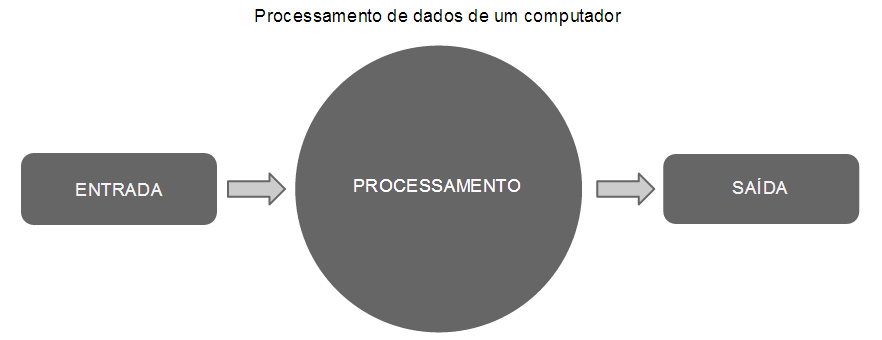
\includegraphics{images/processamento-dados-computador.png}

\subsection{Os Sistemas de Informação e o Mundo dos Negócios}\label{os-sistemas-de-informauxe7uxe3o-e-o-mundo-dos-neguxf3cios}

Em uma visão global, segundo JOAO, BELMIRO NASCIMENTO (2018) os Sistemas de Informação dentro das organizações são

\begin{quote}
soluções para vários problemas e desafios organizacionais. Essa abordagem tem relevância direta para sua carreira, pois \textbf{seus futu­ros empregadores contratarão você por sua habilidade em resolver problemas e atingir objetivos}.(JOÃO, BELMIRO NASCIMENTO - 2018)
\end{quote}

\subsection{A abordagem da resolução de problemas organizacionais}\label{a-abordagem-da-resoluuxe7uxe3o-de-problemas-organizacionais}

No mundo dos negócios as demandas (ou problemas) podem ser agrupados em 3 categorias:

\begin{itemize}
\item
  organização;
\item
  tecnologia;
\item
  pessoas;
\end{itemize}

Segundo \emph{Kenneth C. LAUDON, Jane P. LAUDON,} solucionar probelmas será sempre um processo contínuo de 4 passos:

\begin{enumerate}
\def\labelenumi{\arabic{enumi}.}
\item
  Identificar {[}do problema ou demanda{]};
\item
  Receber as propostas para Solução {[}do problema ou demanda{]};
\item
  Avaliar as propostas e escolher a Solução {[}do problema ou demanda{]};
\item
  Implantar a SOLUÇÂO escolhida {[}para resolver o problema ou demanda{]};
\end{enumerate}

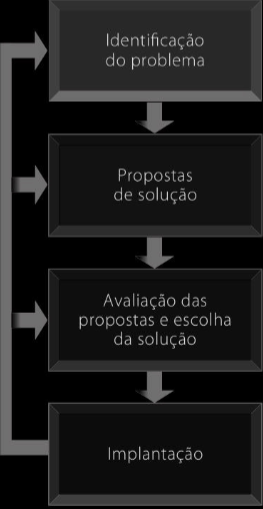
\includegraphics{images/clipboard-3657052893.png}

\begin{longtable}[]{@{}
  >{\raggedright\arraybackslash}p{(\columnwidth - 2\tabcolsep) * \real{0.3625}}
  >{\raggedright\arraybackslash}p{(\columnwidth - 2\tabcolsep) * \real{0.6375}}@{}}
\toprule\noalign{}
\begin{minipage}[b]{\linewidth}\raggedright
Os 4 passos para solucionar problemas (LAUDON e LAUDON)
\end{minipage} & \begin{minipage}[b]{\linewidth}\raggedright
Detalhes
\end{minipage} \\
\midrule\noalign{}
\endhead
\bottomrule\noalign{}
\endlastfoot
1- Identificar {[}problema ou demanda{]} & \begin{minipage}[t]{\linewidth}\raggedright
\begin{itemize}
\item
  Como resolver um problema que não sabemos qual é?
\item
  Os problemas precisam ser definidos pelas pessoas em uma orga­nização antes de serem resolvidos.
\end{itemize}
\end{minipage} \\
2- Propor Solução {[}problema ou demanda{]} & \begin{minipage}[t]{\linewidth}\raggedright
\begin{itemize}
\item
  Identificar soluções viáveis; Custo
\item
  Evitar ``bazuca para matar um pardal'';
\item
  Usar tecnologia ou usar melhor o ``recurso humano'' ?
\end{itemize}
\end{minipage} \\
3- Avaliar Propostas {[}problema ou demanda{]} & \begin{minipage}[t]{\linewidth}\raggedright
\begin{itemize}
\tightlist
\item
  Eficiência vs Eficácia !
\end{itemize}
\end{minipage} \\
4- Implantação {[}problema ou demanda{]} & \begin{minipage}[t]{\linewidth}\raggedright
\begin{itemize}
\tightlist
\item
  Qual a melhor solução ? Geralmente aquela que atende e é mais fácil de ser implantada;
\end{itemize}
\end{minipage} \\
\end{longtable}

\section{Os diferentes Tipos de Sistemas de Informação}\label{os-diferentes-tipos-de-sistemas-de-informauxe7uxe3o}

\textbf{Empresa existe para} (\textbf{cumprir seu propósito} que geralmente é) \textbf{DAR LUCRO} !

\subsubsection{Organizações com fins lucrativos - Empresas}\label{organizauxe7uxf5es-com-fins-lucrativos---empresas}

Uma empresa é uma organização formal cujo ob­ jetivo é produzir produtos ou prestar serviços a fim de obter lu­ cro. E como obter lucro? A conta é simples: vendem-se produtos a um preço superior aos custos da produção.

\subsubsection{Organizações sem fins lucrativos - Fundações Autarquicas - ONGs - Assitência Social - Saúde - Educação - Cultura - Direitos Humanos}\label{organizauxe7uxf5es-sem-fins-lucrativos---fundauxe7uxf5es-autarquicas---ongs---assituxeancia-social---sauxfade---educauxe7uxe3o---cultura---direitos-humanos}

As entidades sem fins lucrativos (dentre as quais estão ONGs ) são organizações que têm como objetivo principal promover o bem-estar social, defender causas ou oferecer serviços à comunidade, sem visar lucro financeiro.

\subsubsection{Organograma de uma Empresa: Uma Representação Visual da Estrutura Organizacional}\label{organograma-de-uma-empresa-uma-representauxe7uxe3o-visual-da-estrutura-organizacional}

Um organograma é uma representação gráfica da estrutura interna de uma organização, mostrando a hierarquia, os cargos, as funções e os departamentos que a compõem. Ele serve como um \textbf{mapa visual} da organização, facilitando a compreensão de \textbf{como as diferentes partes se encaixam} e como o \textbf{poder e a responsabilidade são distribuídos}.

\subsubsection{Organograma Conceitual}\label{organograma-conceitual}

\includegraphics{images/organogramas/organograma-genérico.jpg}

\textbf{Organograma Empresarial - Varejo}

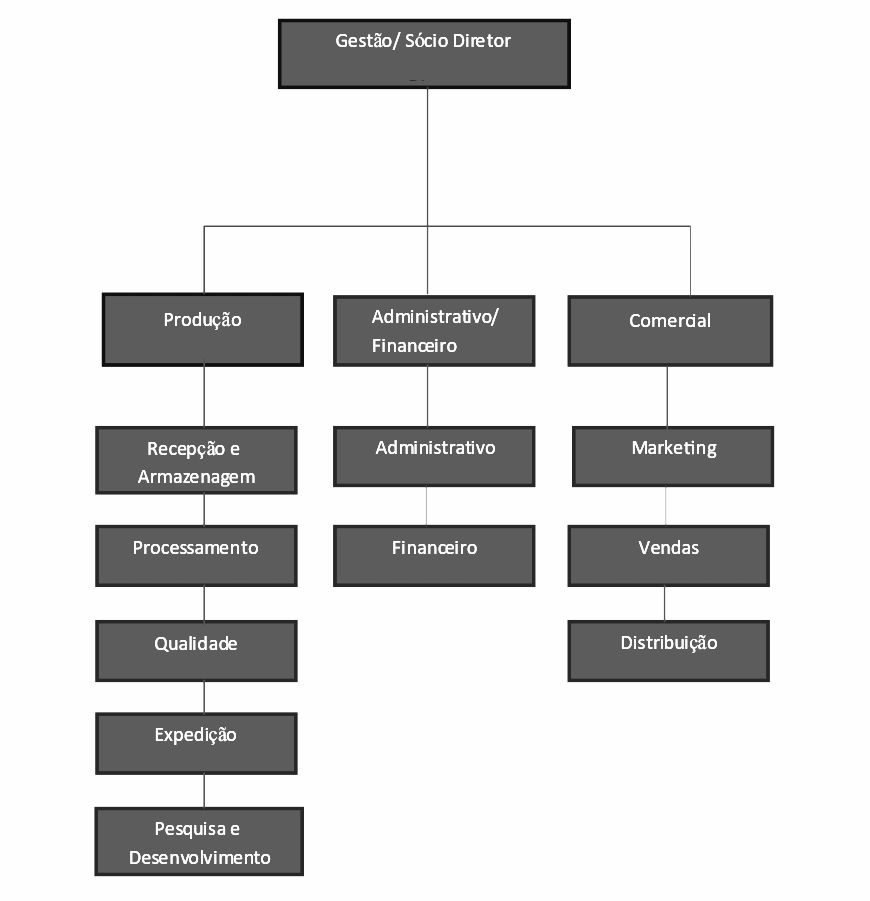
\includegraphics{images/organogramas/Organograma-empresarial.jpg}

\textbf{Organograma Empresarial - Indústria}

Aparece uma ``organela'' responsável por PRODUÇÃO

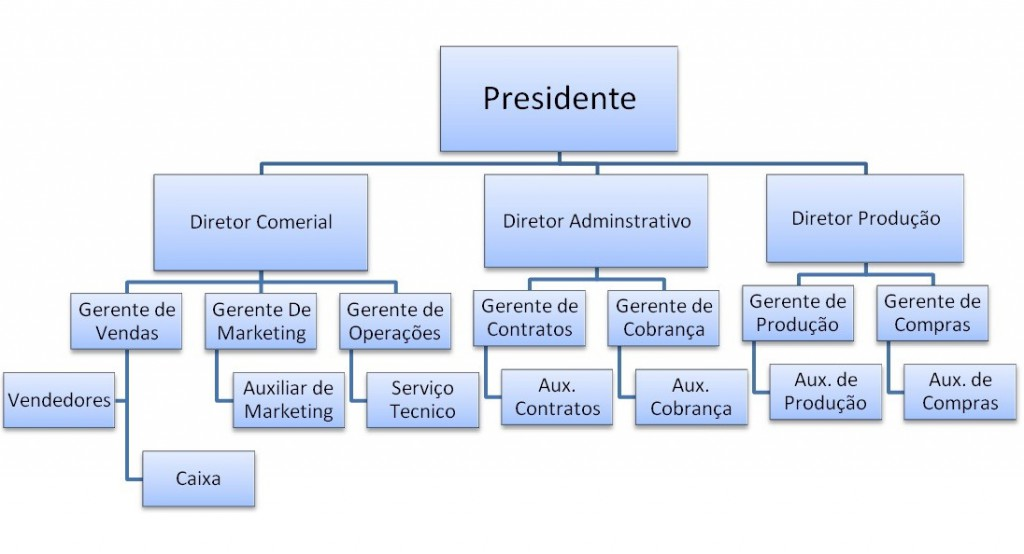
\includegraphics{images/organogramas/OrganogramaIndustrial.jpg}

\textbf{Organograma Organizacional - Organização Sem Fins Lucrativos - Orgão Público}

Exemplo: organograma da Superintendência Estadual de São Paulo do IBGE - Fundação pública da esfera do Poder Executivo Federal

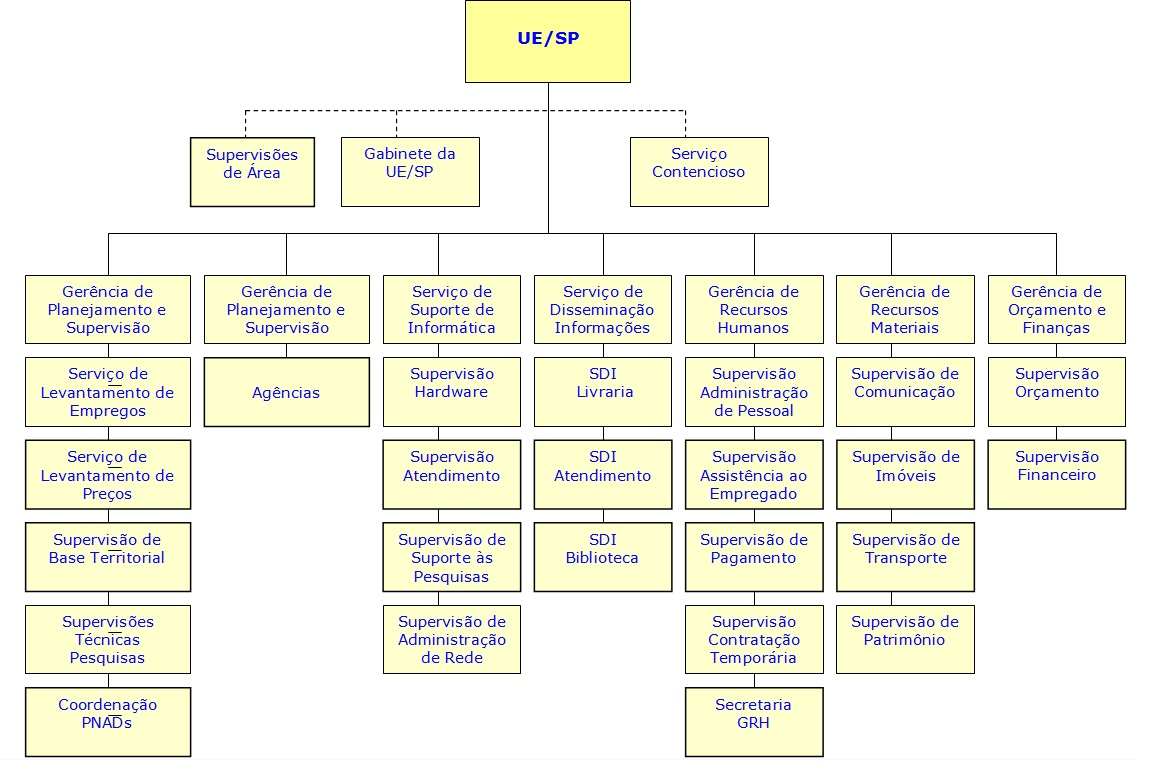
\includegraphics{images/organogramas/SES-SP.jpg}

\textbf{Missão} institucional dessa ``organização'' federal ``\emph{Retratar o Brasil com informações necessárias ao conhecimento de sua realidade e ao exercício da cidadania}''

\subsection{Organizando uma organização tipo empresa: funções empresariais básicas}\label{organizando-uma-organizauxe7uxe3o-tipo-empresa-funuxe7uxf5es-empresariais-buxe1sicas}

Imagine que você queira abrir seu próprio negócio. Você preci­ sará tomar várias decisões: o que produzir ou qual serviço prestar. Essa é uma escolha estratégica, pois vai determinar seus prováveis consumidores, os funcionários de que precisa, os métodos de pro­ dução c muitos outros aspectos. Depois de decidir o que produzir, você deve definir de que tipo de organização vai necessitar. Primeiro, pense em um arranjo de pessoas, máquinas c processos de negócios capaz de produzir. Em segundo lugar, monte uma equipe de marketing e vendas capaz de atrair clientes e vender o produto. Em terceiro, após as vendas, é preciso organizar uma equipe de contabilidade e finanças para cuidar das transações financeiras correntes, como pedidos, faturas e folhas de pagamento. Calma, ainda não acabou: também são necessárias pessoas para cuidar dos assuntos relativos aos funcio­ nários, como recrutamento e capacitação.

Essas quatro funções básicas - que você poderá ver na figura abaixo são encontradas em qualquer empresa. A figura também ajuda a identificar as princi­ pais entidades que formam uma empresa: fornecedores, clientes, funcionários, os salários que ela paga e, é claro, os produtos e serviços que produz.

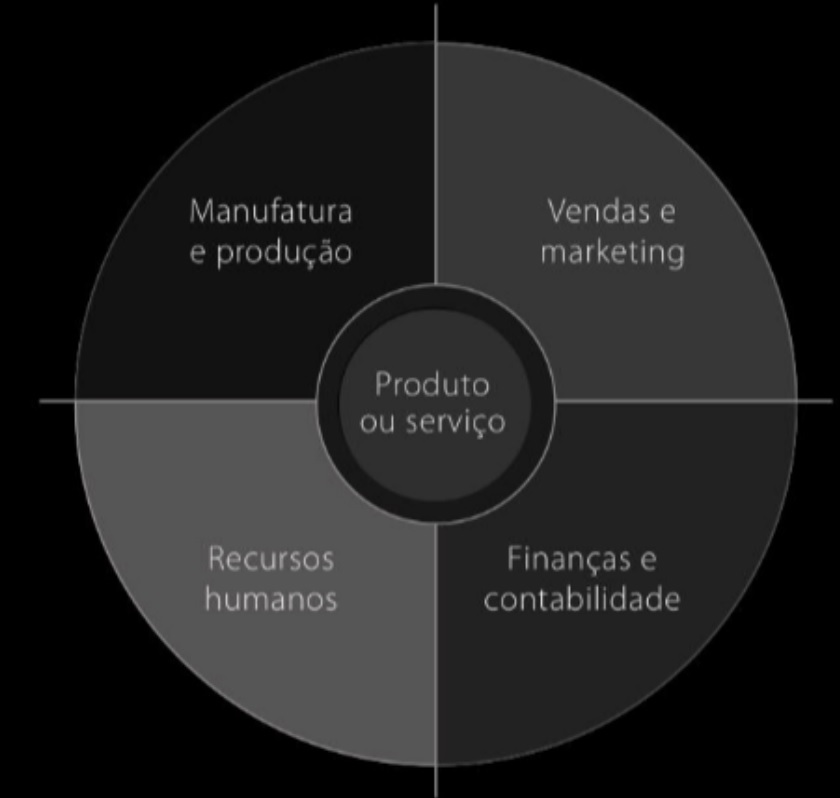
\includegraphics{images/1-dados-info/AreasBasicasEmpresa.jpg}

Fonte: adaptada de Laudon e Laudon (2011, página 37).

\begin{quote}
Organização -\textgreater{} Conhecimento do Negócio -\textgreater{} Processos Mapeados -\textgreater{} Sistema de Informação Mapeado
\end{quote}

\includegraphics{images/1-dados-info/ProcessosNegócioMapeados.jpg}

Processos do Cliclo de Vida da Produção de um produto (Indústria)

\section{Sistemas de Informação e Vantagem Competitiva}\label{sistemas-de-informauxe7uxe3o-e-vantagem-competitiva}

As empresas que se destacam em seus setores geralmente possuem algum tipo de \texttt{vantagem\ competitiva}.

As vantagens competitivas podem vir de dois aspectos a seguir:

\begin{itemize}
\item
  \textbf{recursos especiais};
\item
  \textbf{uso mais eficiente desses recursos};
\end{itemize}

\begin{longtable}[]{@{}
  >{\raggedright\arraybackslash}p{(\columnwidth - 6\tabcolsep) * \real{0.6667}}
  >{\centering\arraybackslash}p{(\columnwidth - 6\tabcolsep) * \real{0.1042}}
  >{\centering\arraybackslash}p{(\columnwidth - 6\tabcolsep) * \real{0.1042}}
  >{\centering\arraybackslash}p{(\columnwidth - 6\tabcolsep) * \real{0.1042}}@{}}
\toprule\noalign{}
\begin{minipage}[b]{\linewidth}\raggedright
Vantagem / Sistemas de Informação
\end{minipage} & \begin{minipage}[b]{\linewidth}\centering
SI ERP
\end{minipage} & \begin{minipage}[b]{\linewidth}\centering
SI SCM
\end{minipage} & \begin{minipage}[b]{\linewidth}\centering
SI CRM
\end{minipage} \\
\midrule\noalign{}
\endhead
\bottomrule\noalign{}
\endlastfoot
\textbf{Excelência operacional;} & ALTA & ALTA & ALTA \\
\textbf{Novos produtos, serviços e modelos de negócios;} & MÉDIA & SIM & SIM \\
\textbf{Relacionamento mais estreito com clientes e fornecedores;} & MÉDIA & ALTA & ALTA \\
\textbf{Melhor tomada de decisões;} & EXTREMA & ALTA & ALTA \\
\textbf{Sobrevivência no mercado;} & ALTA & ALTA & ALTA \\
\end{longtable}

\section{Tipos de sistemas de informação empresariais}\label{tipos-de-sistemas-de-informauxe7uxe3o-empresariais}

\begin{enumerate}
\def\labelenumi{\arabic{enumi}.}
\item
  \texttt{Sistemas\ de\ processamento\ de\ transações\ (SPTs)}; Monitoramento de pedidos de expedição de mercadoria; Monitoramento de pedidos de atendimento;
\item
  \texttt{Sistemas\ de\ informações\ gerenciais\ (SIGs)}; Relatório de faltas de funcionário; Relatório de mercadorias com defeito;
\item
  \texttt{Sistemas\ de\ apoio\ à\ decisão\ (SADs)}; Sistemas Business Inteligence;
\item
  \texttt{Sistemas\ de\ apoio\ ao\ executivo\ (SAEs)}; Relatório de vendas consolidado aos acionistas; Relatório de competitividade;
\item
  \textbf{Sistemas integrados (ERP);} Gestão e colaboração departamentos;
\item
  \textbf{Sistemas de gestão da cadeia de suprimentos (SCM);} Monitoramento de entrega de vendas on-line; Monitoramento Drop-Shipping;
\item
  \textbf{Sistemas de gestão do relacionamento com o cliente (CRM);} Relatório de satisfação de clientes; Relatório de Retenção de Clientes;
\item
  \textbf{Sistemas de gestão do conhecimento (SGCs);} Sistemas ITL; Sistemas de prestação de suporte técnico;
\end{enumerate}

\subsection{Sistemas integrados (E.R.P. - Planejamento de Recursos Empresariais ou Enterprise Resource Planning )}\label{sistemas-integrados-e.r.p.---planejamento-de-recursos-empresariais-ou-enterprise-resource-planning}

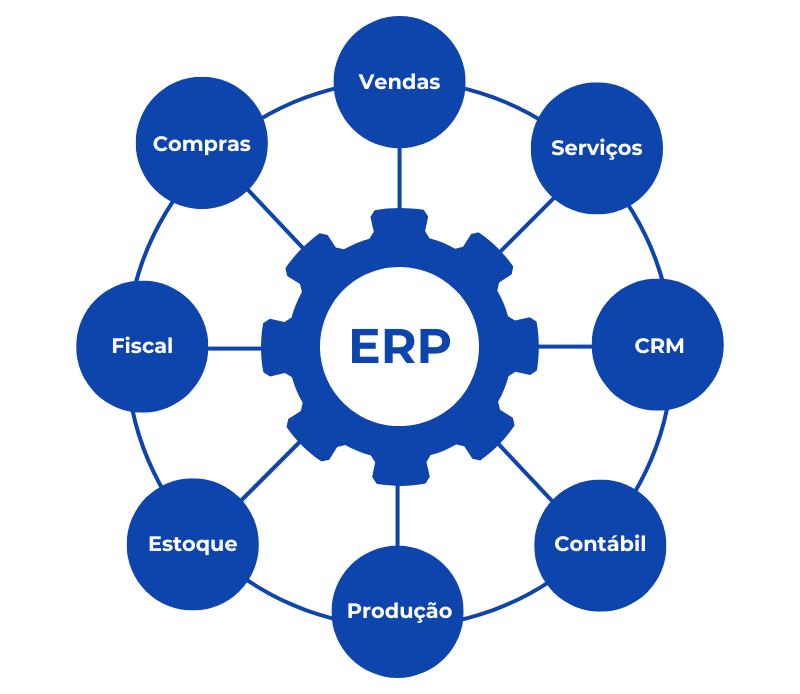
\includegraphics[width=6.28125in,height=\textheight]{images/sistemas/erp.png}

O termo ERP foi cunhado pelo Gartner Group em 1990. Um sistema ERP, segundo Davenport (1998)

\begin{quote}
'' \textbf{\emph{ERP é um sistema de software que integra todas as áreas funcionais de uma empresa, desde finanças e contabilidade até produção e vendas.}} '' Davenport, T. H. (1998). Putting the enterprise into the enterprise system. Harvard business review, 76(4), 121-131.
\end{quote}

As principais funções de um sistema ERP em empresas do varejo são:

\begin{itemize}
\item
  Centralizar a gestão operacional
\item
  Gerir o estoque e os suprimentos
\item
  Emitir notas fiscais
\item
  Controlar as finanças
\item
  Cadastrar clientes e produtos
\item
  Administrar a empresa
\end{itemize}

Alguns exemplos de SIs ERPs, em 2025, são:

\begin{itemize}
\item
  Pacote \href{https://www.sap.com/brazil/products/erp.html}{SAP ERP};
\item
  Pacote \href{https://www.oracle.com/br/erp/}{Oracle ERP Cloud};
\item
  Pacote \href{https://www.microsoft.com/pt-br/dynamics-365/pricing-overview}{Microsoft Dynamics 365};
\item
  Pacote \href{https://www.infor.com/pt-br}{Infor ERP};
\item
  Pacote \href{https://www.netsuite.com/portal/br/products/erp.shtml}{NetSuite ERP};
\item
  Sistema ERP \href{https://www.totvs.com/sistema-de-gestao/}{TOTVS};
\item
  Sistema ERP Web \href{https://www.bling.com.br/}{BLING};
\end{itemize}

\subsection{Sistemas de gestão da cadeia de suprimentos (supply chain management - SCM)}\label{sistemas-de-gestuxe3o-da-cadeia-de-suprimentos-supply-chain-management---scm}

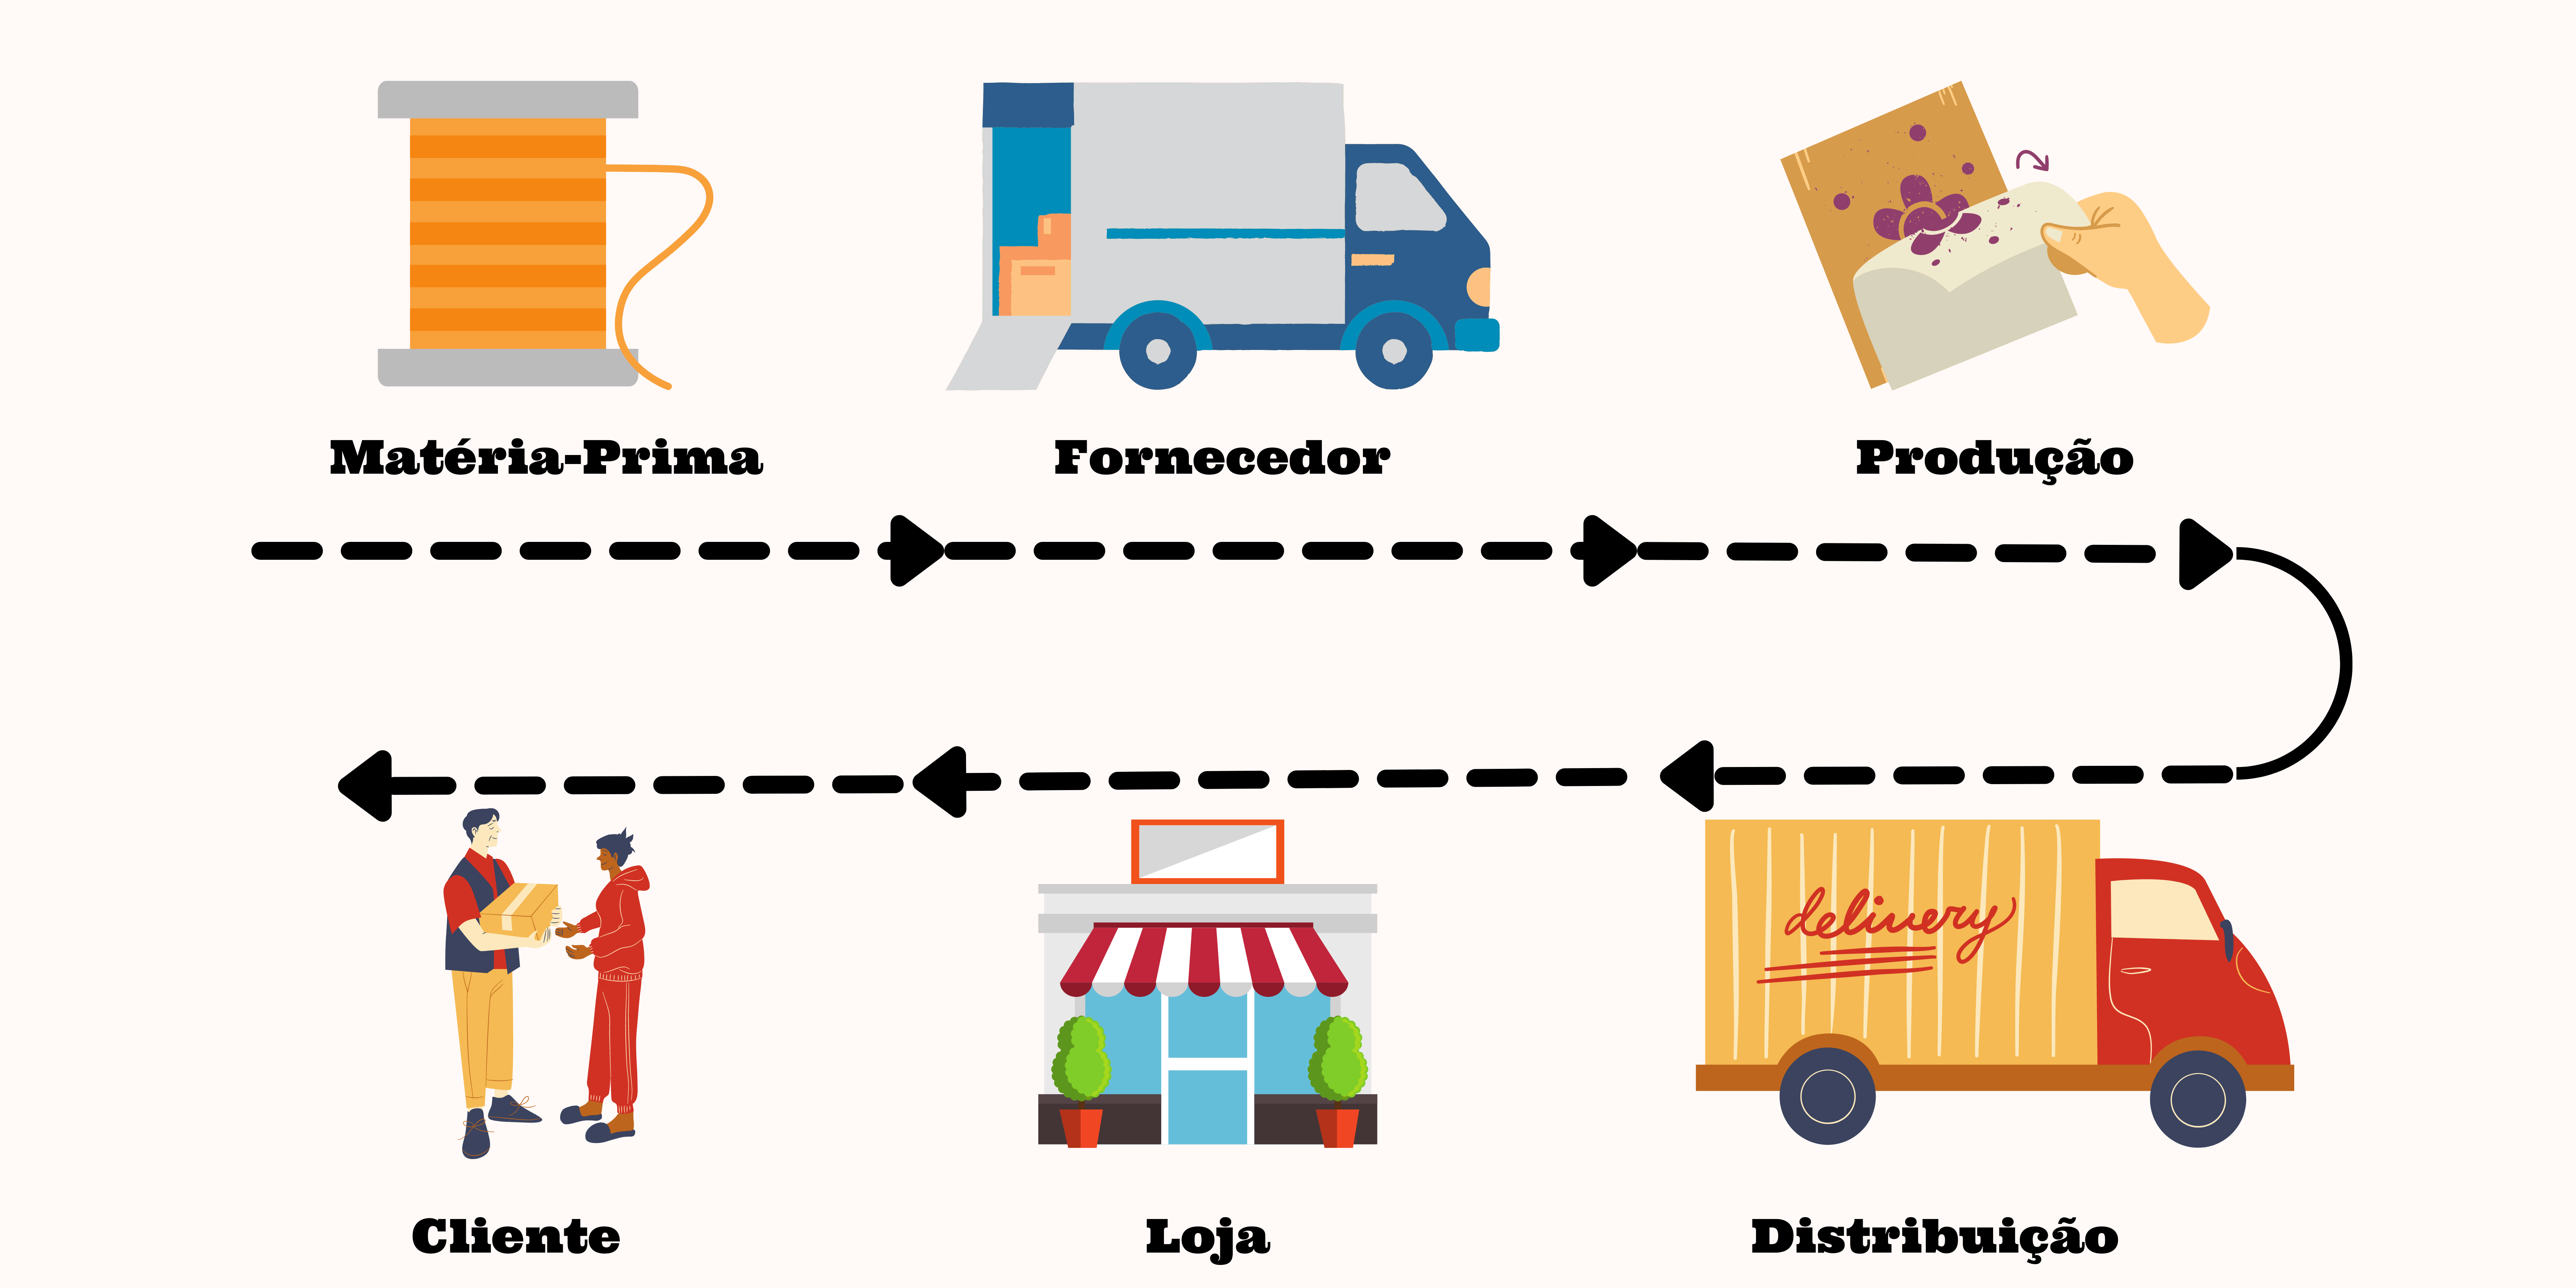
\includegraphics[width=7.4375in,height=\textheight]{images/sistemas/SCM.png}

Os SI SCM são ferramentas essenciais para otimizar o fluxo de produtos, informações e finanças desde a origem até o consumidor final. Eles abrangem todas as etapas da cadeia de suprimentos, desde a aquisição de matérias-primas até a entrega do produto final ao cliente.

Segundo Simchi-Levi, D., Kaminsky, P., \& Simchi-Levi, E. (2008)

\begin{quote}
\textbf{\emph{SCMé um SI que faz um conjunto de abordagens utilizadas para INTEGRAR eficientemente FORNECEDORES, ARMAZENS e LOJAS, de modo que as MERCADORIAS sejam PRODUZIDAS e DISTRIBUÍDAS nas QUANTIDADES certas, para os LOCAIS certos e nos MOMENTOS certos, a fim de MINIMIZAR os CUSTOS de todo o sistema, satisfazendo os requisitos de nível de serviço.}} Designing and managing the supply chain: concepts, strategies, and case studies de David Simchi-Levi, Philip Kaminsky e Edith Simchi-Levi. (2008)
\end{quote}

As principais funções de um SI SCM são:

\begin{itemize}
\item
  Reduzir custos: Otimizando processos, estoques e transportes.
\item
  Melhorar a eficiência: Agilizando o fluxo de produtos e informações.
\item
  Aumentar a satisfação do cliente: Garantindo entregas no prazo e produtos de qualidade.
\item
  Otimizar toda a cadeia de suprimentos: Interligando todas as etapas, desde fornecedores até clientes.
\end{itemize}

Alguns exemplos de SIs SCMs, em 2025, são:

\begin{itemize}
\item
  Oracle SCM Cloud;
\item
  SAP SCM;
\item
  Blue Yonder (JDA Software);
\end{itemize}

\subsection{Sistemas de Relacionamento com Cliente - CRM (Customer Relationship Management)}\label{sistemas-de-relacionamento-com-cliente---crm-customer-relationship-management}

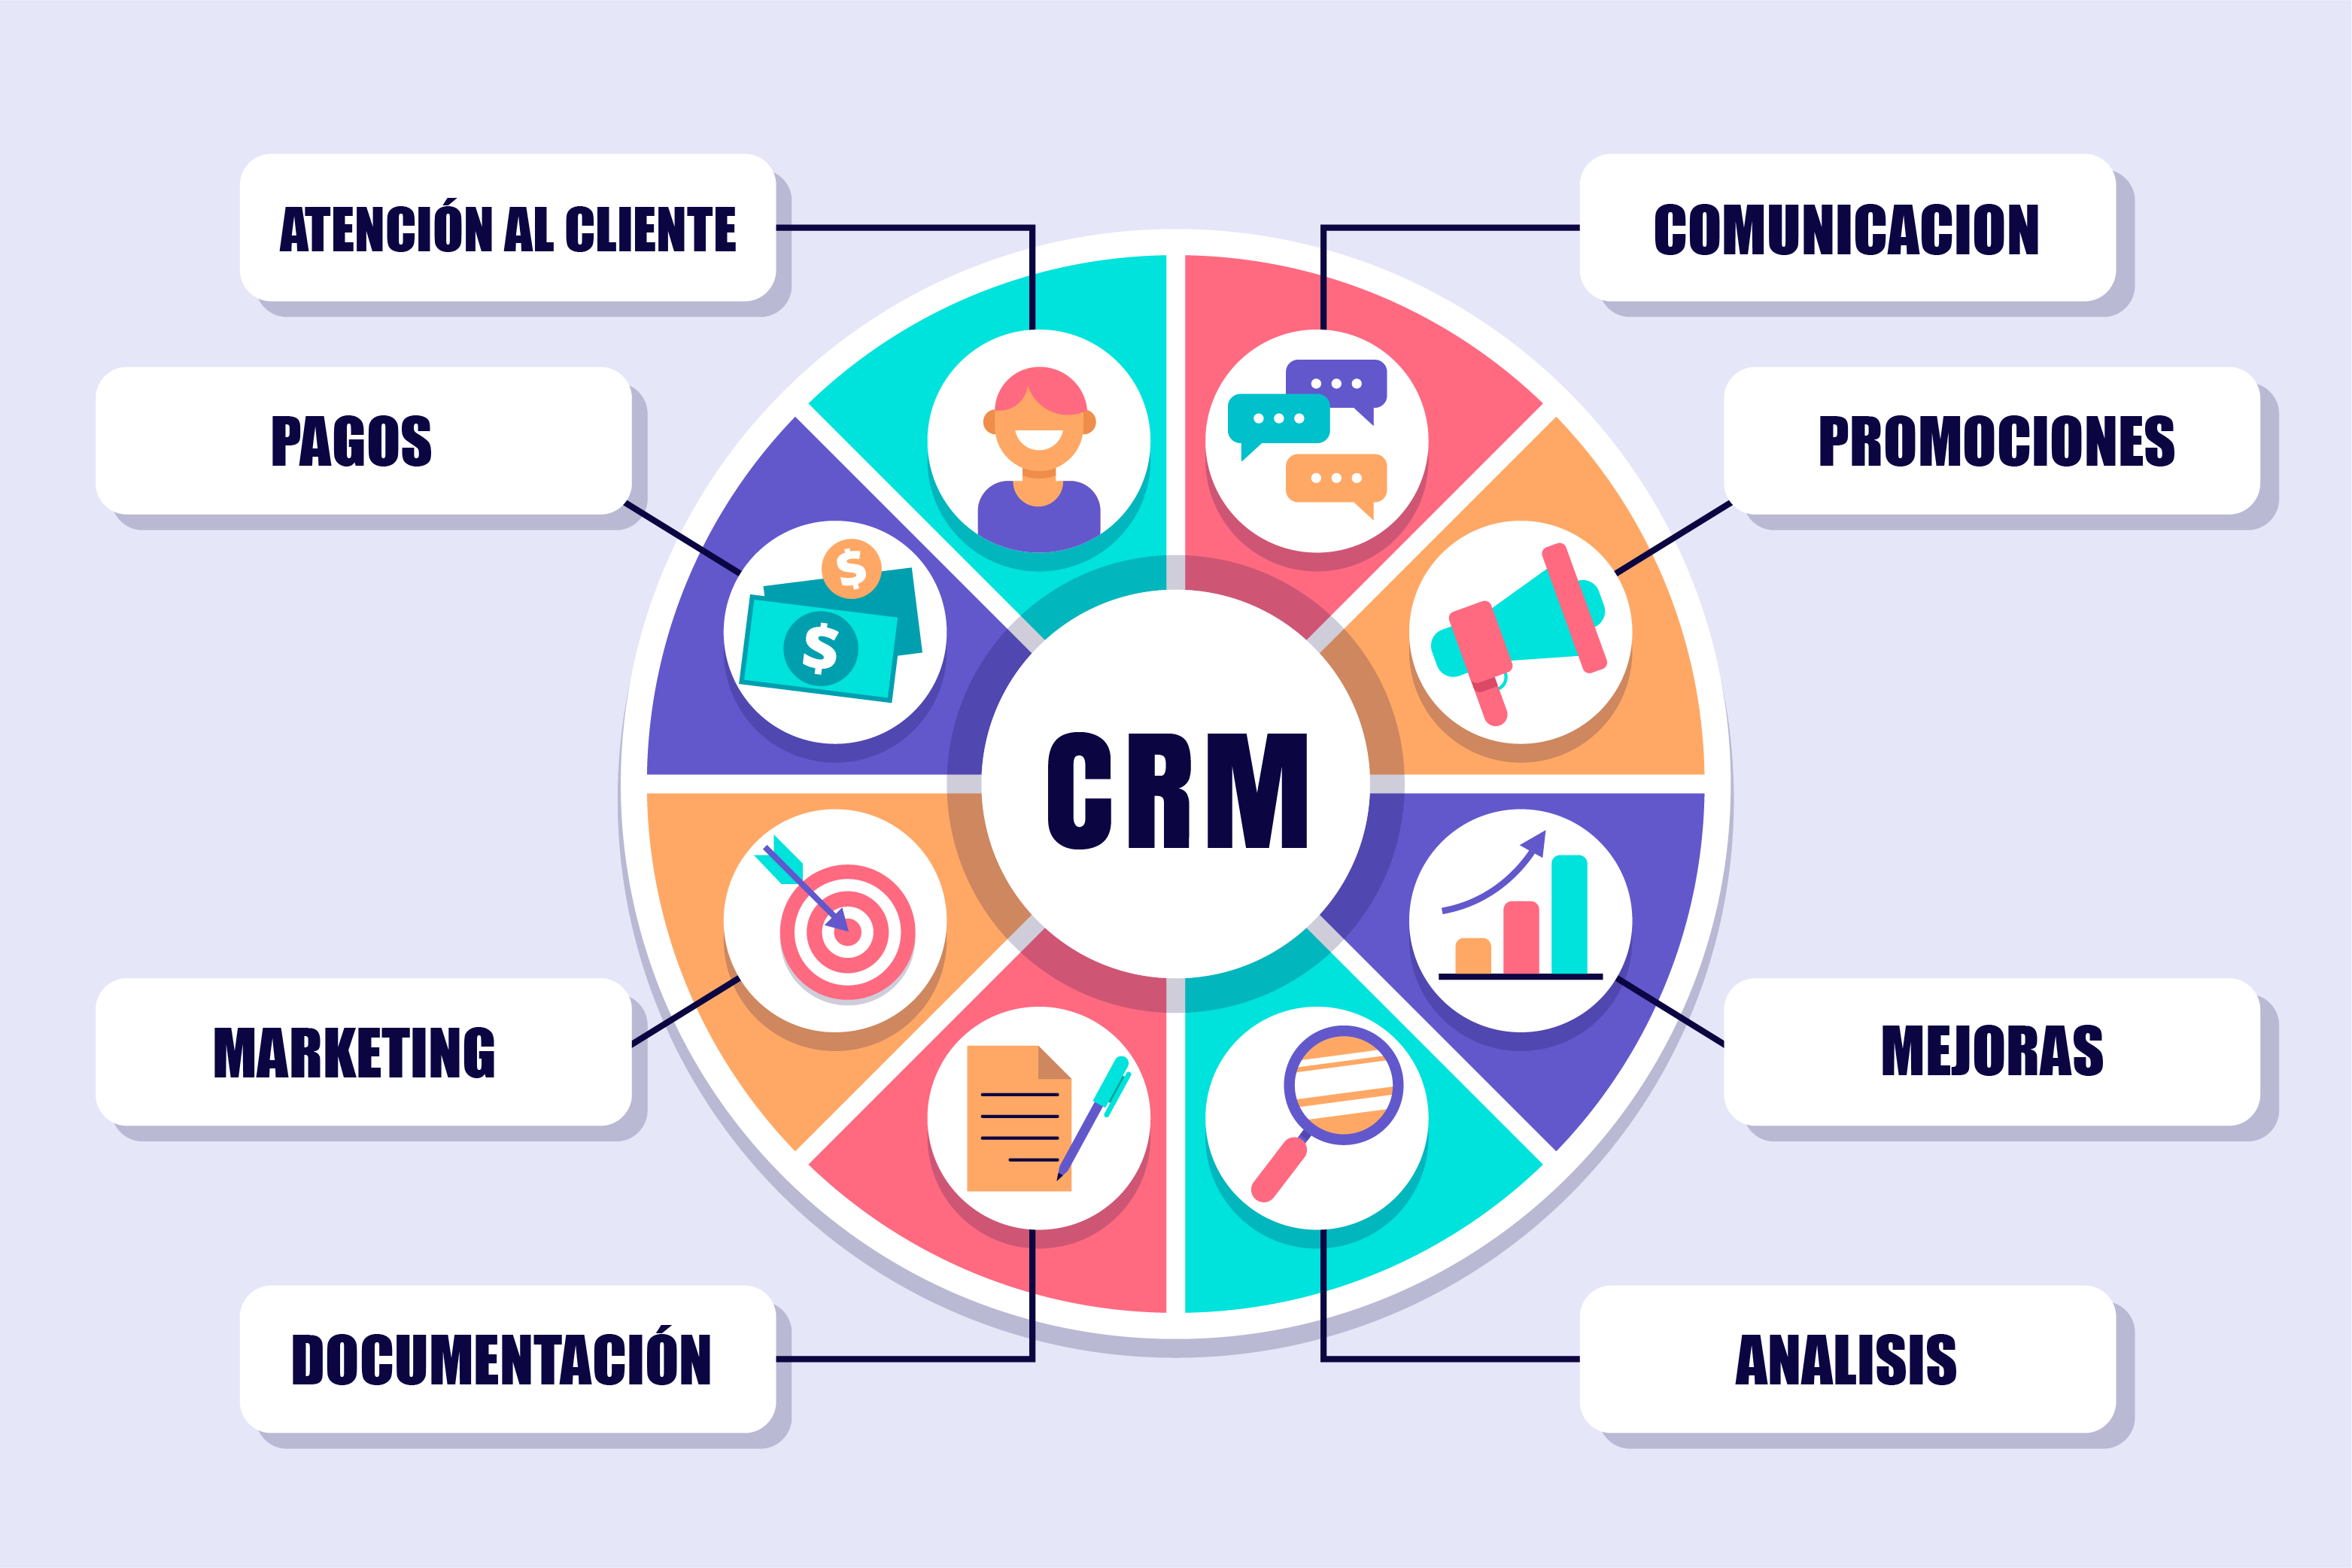
\includegraphics[width=6.6875in,height=\textheight]{images/sistemas/CRM.png}

São SIs de análise de clientes, com o objetivo de melhorar o relacionamento, aumentar a fidelização e impulsionar as vendas. Segundo Kotler, P., \& Keller, K. L. (2016), um um CRM pode ser definido assim

\begin{quote}
\textbf{\emph{Um SI CRM implanta o processo de gerenciar informações detalhadas sobre clientes individuais e gerenciar cuidadosamente todos os pontos de contato do cliente para maximizar a lealdade do cliente.}} Kotler, P., \& Keller, K. L. (2016). Marketing management
\end{quote}

As principais funções de um SI CRM são:

\begin{itemize}
\item
  Coleta e organização de dados: Reunindo informações sobre clientes, histórico de compras, interações e preferências.
\item
  Automação de processos: Otimizando tarefas de marketing, vendas e atendimento ao cliente.
\item
  Análise de dados: Identificando padrões e insights para melhorar a tomada de decisões.
\item
  Personalização do atendimento: Oferecendo experiências individualizadas aos clientes.
\end{itemize}

Alguns exemplos de SIs CRMs, em 2025, são:

\begin{itemize}
\item
  Salesforce CRM;
\item
  Microsoft Dynamics 365;
\item
  HubSpot CRM;
\item
  Zendesk Sell;
\end{itemize}

\section{Exercícios}\label{exercuxedcios}

\section{Questões}\label{questuxf5es}

\begin{enumerate}
\def\labelenumi{\arabic{enumi}.}
\item
  Qual o \textbf{papel dos sistemas de informação no ambiente de negócios contemporâneo}?
\item
  Quais são os \textbf{objetivos organizacionais dos sistemas de informação}?
\item
  Qual a \textbf{diferença entre dados e informações}?
\item
  Quais são as \textbf{atividades básicas em um sistema de informação}?
\item
  O que são \textbf{abordagens de resolução de problemas organizacionais} e como aplicá-las?
\item
  O que é uma \textbf{empresa} e quais os seus componentes?
\item
  Quais as \textbf{funções básicas de uma empresa}?
\item
  Quais os \textbf{níveis hierárquicos de uma empresa}?
\item
  Quais os \textbf{tipos de sistemas de informação empresariais}?
\item
  O que é \textbf{colaboração}?
\item
  Qual a \textbf{função dos sistemas de informação em uma empresa}?
\item
  Como usar os \textbf{sistemas de informação para conquistar vantagem competitiva}?
\end{enumerate}

\section{Testes múltipla escolha}\label{testes-muxfaltipla-escolha}

\textbf{1. Qual das seguintes alternativas descreve melhor o propósito e a função de um Sistema de Planejamento de Recursos Empresariais (ERP)?}

\begin{enumerate}
\def\labelenumi{\alph{enumi})}
\item
  Um sistema ERP é utilizado principalmente para gerenciar o relacionamento com os clientes, coletando e analisando dados de interações para melhorar as vendas e o atendimento ao cliente.
\item
  Um sistema ERP foca-se na gestão da cadeia de suprimentos, coordenando atividades entre fornecedores, fabricantes e distribuidores para otimizar o fluxo de produtos.
\item
  Um sistema ERP é projetado para capturar e aplicar conhecimento dentro da organização, facilitando a criação, o armazenamento e a transferência de expertise entre os funcionários.
\item
  Um sistema ERP integra processos de negócios em áreas como manufatura, finanças, vendas e recursos humanos em um único sistema de software, permitindo o acesso e o compartilhamento de informações em toda a organização.
\item
  Um sistema ERP serve para analisar dados históricos e atuais da empresa, a fim de identificar tendências de mercado e prever o comportamento do consumidor.
\end{enumerate}

\textbf{2. Qual das seguintes alternativas descreve melhor a função de um sistema de informação (SI) em uma empresa?}

\begin{enumerate}
\def\labelenumi{\alph{enumi})}
\item
  Um SI serve principalmente para gerenciar a cadeia de suprimentos, otimizando o fluxo de produtos desde os fornecedores até os clientes.
\item
  Um SI tem como principal função coletar dados brutos e não organizados sobre as operações da empresa.
\item
  Um SI é um conjunto de componentes relacionados que coletam, processam, armazenam e distribuem informações para apoiar a tomada de decisões, a coordenação e o controle da organização.
\item
  Um SI é usado para transformar dados em informações úteis, apresentando-os de forma organizada e compreensível.
\item
  Um SI é utilizado principalmente para integrar todos os processos de negócios da empresa em um único sistema de software, facilitando o acesso e o compartilhamento de dados.
\end{enumerate}

\section{Respostas questões:}\label{respostas-questuxf5es}

\begin{enumerate}
\def\labelenumi{\arabic{enumi}.}
\tightlist
\item
  Qual o \textbf{papel dos sistemas de informação no ambiente de negócios contemporâneo}?
\end{enumerate}

\textbf{Resposta}: Ajudar a atingir Objetivos organizacionais, promover a transformação do negócio, promover integração e colaboração das áreas, criar Vantagem competitiva e, finalmente, ajudar na tomada de decisões.

\begin{enumerate}
\def\labelenumi{\arabic{enumi}.}
\setcounter{enumi}{1}
\tightlist
\item
  Quais são os \textbf{objetivos organizacionais dos sistemas de informação}?
\end{enumerate}

\textbf{Resposta}: Promover excelência operacional, possibilitar novos produtos e modelos de negócio, ajudar o relacionamento entre clientes e fornecedores.

\begin{enumerate}
\def\labelenumi{\arabic{enumi}.}
\setcounter{enumi}{2}
\tightlist
\item
  Qual a \textbf{diferença entre dados e informações}?
\end{enumerate}

\textbf{Resposta}: Dados são sequência de informações ainda não analisados. Informações são dados apresentados de forma útil.

\begin{enumerate}
\def\labelenumi{\arabic{enumi}.}
\setcounter{enumi}{3}
\tightlist
\item
  Quais são as \textbf{atividades básicas em um sistema de informação}?
\end{enumerate}

\textbf{Resposta}: Entrada, Processamento e Saída.

\begin{enumerate}
\def\labelenumi{\arabic{enumi}.}
\setcounter{enumi}{4}
\tightlist
\item
  O que são \textbf{abordagens de resolução de problemas organizacionais} e como aplicá-las?
\end{enumerate}

\textbf{Resposta}: Identificar Problema, Propor Solução, Escolher Solução, Implantar Solução.

\begin{enumerate}
\def\labelenumi{\arabic{enumi}.}
\setcounter{enumi}{5}
\tightlist
\item
  O que é uma \textbf{empresa} e quais os seus componentes?
\end{enumerate}

\textbf{Resposta}: Uma empresa é uma organização formal cujo objetivo é produzir produtos ou prestar serviços a fim de obter lucro. Seus componentes são CLIENTES, FORNECEDORES, FUNCIONÁRIOS, PRODUTOS E SERVIÇOS.

\begin{enumerate}
\def\labelenumi{\arabic{enumi}.}
\setcounter{enumi}{6}
\tightlist
\item
  Quais as \textbf{funções básicas de uma empresa}?
\end{enumerate}

\textbf{Resposta}: Manufatura e produção, Vendas e marketing, Recursos humanos e; Finanças e Contabilidade.

\begin{enumerate}
\def\labelenumi{\arabic{enumi}.}
\setcounter{enumi}{8}
\tightlist
\item
  Quais os \textbf{níveis hierárquicos de uma empresa}?
\end{enumerate}

\textbf{Resposta}: Gerência sênior (Conselho Diretor e Presidente), Gerência média (Diretores), Gerência operacional (Gerentes), Trabalhadores do conhecimento (analistas setoriais), Trabalhadores de dados (analistas setoriais), Trabalhadores dos serviços ou da produção (chão-de-fábrica).

\begin{enumerate}
\def\labelenumi{\arabic{enumi}.}
\setcounter{enumi}{9}
\tightlist
\item
  Quais os \textbf{tipos de sistemas de informação empresariais}?
\end{enumerate}

\textbf{Resposta}: Sistemas integrados (ERP), Sistemas de gestão da cadeia de suprimentos (SCM), Sistemas de gestão do relacionamento com o cliente (CRM) e Sistemas de gestão do conhecimento (SGCs).

\begin{enumerate}
\def\labelenumi{\arabic{enumi}.}
\setcounter{enumi}{10}
\tightlist
\item
  O que é \textbf{colaboração}?
\end{enumerate}

\textbf{Resposta}: colaboração é o trabalho com os outros para alcançar metas claras e compartilhadas.

\begin{enumerate}
\def\labelenumi{\arabic{enumi}.}
\setcounter{enumi}{11}
\tightlist
\item
  Qual a \textbf{função dos sistemas de informação em uma empresa}?
\end{enumerate}

\textbf{Resposta}: Coletar (ou Recuper), Processar, Armazenar e distribuir INFORMAÇÕES.

\begin{enumerate}
\def\labelenumi{\arabic{enumi}.}
\setcounter{enumi}{12}
\tightlist
\item
  Como usar os \textbf{sistemas de informação para conquistar vantagem competitiva}?
\end{enumerate}

\textbf{Resposta}: Melhorando a gestão de processos de negócios.

\section{Respostas dos testes:}\label{respostas-dos-testes}

\begin{longtable}[]{@{}cc@{}}
\toprule\noalign{}
Questão & Resposta \\
\midrule\noalign{}
\endhead
\bottomrule\noalign{}
\endlastfoot
1 & D \\
2 & C \\
\end{longtable}

\chapter{Apresentação Trabalho NP1}\label{apresentauxe7uxe3o-trabalho-np1}

Este trabalho substitui a primeira prova (NP1) do primeiro bimestre de 2025.

Este trabalho levará o aluno a fazer um estudo de mercado para obter financiamento de um investidor para montar uma EMPRESA/CONSULTORIA DE IMPLANTAÇÃO DE ERPs de terceiros.

Dinâmica: o trabalho será desenvolvido em grupo de até 4 alunos (o grupo simulará uma startup).

O trabalho deve ser entregue impresso em tamanho A4, uma cópia por aluno (como se fosse individual).

O trabalho deverá ter no mínimo 5 e no máximo 10 folhas.

\section{NP1 -- TRABALHO DE SUBSTITUIÇÃO DE PROVA P1 - PESQUISA}\label{np1-trabalho-de-substituiuxe7uxe3o-de-prova-p1---pesquisa}

\subsection{1- CAPA}\label{capa}

\textbf{UNIP} -- UNIVERSIDADE PAULISTA

\textbf{CURSO}: TECNOLOGIA EM ANÁLISE E DESENVOLVIMENTO DE SISTEMAS

\textbf{DISCIPLINA} -- TIC -- TECNOLOGIA DA INFORMAÇÃO E TELECOMUNICAÇÃO

\textbf{TÍTULO}: PLANO Captação de Investimento para empresa ``CONSULTORIA E IMPLANTAÇÃO ERP+ COMERCIO ELETRÔNICO'' - GRUPO número ``x'' {[}onde x é definido pelo professor{]}

\begin{itemize}
\tightlist
\item
  NOME: Integrante 1
  NOME: Integrante 2 NOME: Integrante 3 NOME: Integrante 4
\end{itemize}

\textbf{PROFESSOR}: Miguel Suez Xve Penteado

\subsection{2- Agradecimentos e dedicatórias:}\label{agradecimentos-e-dedicatuxf3rias}

NÃO VAI FAZER

\subsection{3- Sumário:}\label{sumuxe1rio}

( introdução pág x , justificativa pág y, objetivo pág z \ldots{} )

\subsection{4- Resumo:}\label{resumo}

``ESTE ESTUDO DO GRUPO X PROVOU QUE UMA EMPRESA DO RAMO DE CONSULTORIA E IMPLANTAÇÃO DE SOLUÇÃO ERP + COMERCIO ELETRÔNICO É VIAVEL, SEGUNDO LEVANTAMENTO DAS PESQUISAS X,Y,Z DO(S) ORGÃO(S) X(Y,Z)''

\subsection{5-Justificativa:}\label{justificativa}

`` UMA VEZ COMPROVADA A DEMANDA POR IMPLANTAÇÃO DE SOFTWARE TIC ERP E CRM + SCM (REPRESENTADAS SUAS FUNCIONALIDADES NO E-COMERCE), JUSTIFICA-SE O INVESTIMENTO EM STARTUPs DESTA NAUTREZA''

\subsection{6-Objetivo:}\label{objetivo}

LEVANTAR OS DADOS QUE PROVAM AO INVESTIDOR QUE COMPENSA INVESTIR EM UMA STARTUP DE IMPLANTAÇÃO DE Sis ERP+E-COMERCE.

\subsection{7 -- introdução}\label{introduuxe7uxe3o}

SOMOS O GRUPO X, NOSSO GRUPO IMPLANTA ERPs INTEGRADOS A COMERCIO ELETRÔNICO. MAS O QUE VEM A SER UM ERP ? {[}EXPLICA O QUE É UM ERP SEGUNDO NOSSOS LIVROS TEXTO{]}. E O QUE É COMERCIO ELETRÔNICO ? {[}EXPLICA{]}. QUAL A VANTAGEM COMPETITIVA DE UMA EMPRESA QUE TEM ESSES SI(s) ? {[}EXPLICA E PODE USAR OS NOSSOS LIVROS-TEXTO COMO REFERÊNCIA{]}

\subsection{8- Revisão Bibliográfica:}\label{revisuxe3o-bibliogruxe1fica}

``EMPRESAS DE CONSULTORIA EM TIC PARA IMPLANTAÇÃO DE SISTEMAS TIPO ERP E COMERCIO ELETRÔNICO DÃO LUCRO EM 2025. SEGUNDO AS ÚLTIMAS PESQUISAS \ldots. FOI COMPROVADO A NECESSIDADE DA POPULAÇÃO EM TAL TIPO DE SOFTWARE, E POR CONSEQUÊNCIA, EMPRESAS QUE IMPLANTAM ESSE TIPO DE SOFTWARE DÃO LUCRO\ldots{}''

Segundo \textbf{A PESQUISA 1} -- TANTAS EMPRESAS SE INFORMATIZARAM NOS ULTIMOS 5 ANOS.., SEGUNDO \textbf{A PESQUISA 2}, TANTAS PESSOAS COMPRARAM DA INTERNET NOS ULTIMOS 5 ANOS. SEGUNDO \textbf{A PESQUISA 3}, HÁ TANTAS PESSOAS BUSCANDO ENSINO A DISTÂNCIA

\subsection{9-Materiais e Métodos}\label{materiais-e-muxe9todos}

COLHI TAL \textbf{DADO}, E CHEGUEI A TAL \textbf{INFORMAÇÃO} DE TAL PESQUISA;

\subsection{10-Resultados}\label{resultados}

PODEMOS CONCLUIR O \textbf{CONHECIMENTO1} DE QUE \ldots{} A PARTIR DA \textbf{INFORMAÇÃO1};

PODEMOS CONCLUIR O \textbf{CONHECIMENTO2} DE QUE \ldots{} A PARTIR DA \textbf{INFORMAÇÃO2};

PODEMOS CONCLUIR O \textbf{CONHECIMENTO3} DE QUE \ldots{} A PARTIR DA \textbf{INFORMAÇÃO3};

\subsection{11- Discussão}\label{discussuxe3o}

O \textbf{CONHECIMENTO1} JUSTIFICA O INVESTIMENTO NA NOSSA STARTUP DO GRUPO X, QUE IMPLANTA Sis ERP+COMÉRCIO ELETRÔNICO;

O \textbf{CONHECIMENTO2} JUSTIFICA O INVESTIMENTO NA NOSSA STARTUP DO GRUPO X, QUE IMPLANTA Sis ERP+COMÉRCIO ELETRÔNICO;

\subsection{12-Conclusão}\label{conclusuxe3o}

POR ISSO TUDO, OU SEJA CONHECIMENTO1, CONHECIMENTO2, CONHECIMENTO3\ldots{} COMPROVAMOS QUE COMPENSA O IVESTIMENTO NA EMPRESA DO GRUPO X. CONVIDO VOCÊ A SER NOSSO SÓCIO;

\subsection{13-Referencias Bibliográficas}\label{referencias-bibliogruxe1ficas}

PESQUISA 1\ldots{}

PESQUISA 2\ldots{}

PESQUISA 3\ldots{}

\subsection{Apendice - links de pesquisas de TIC no Brasil}\label{apendice---links-de-pesquisas-de-tic-no-brasil}

\begin{longtable}[]{@{}
  >{\centering\arraybackslash}p{(\columnwidth - 2\tabcolsep) * \real{0.4444}}
  >{\raggedright\arraybackslash}p{(\columnwidth - 2\tabcolsep) * \real{0.5556}}@{}}
\caption{Pesquisas TIC do CETIC (NIC.br)}\tabularnewline
\toprule\noalign{}
\begin{minipage}[b]{\linewidth}\centering
Pesquisa do CETIC - NIC.br
\end{minipage} & \begin{minipage}[b]{\linewidth}\raggedright
Endereço
\end{minipage} \\
\midrule\noalign{}
\endfirsthead
\toprule\noalign{}
\begin{minipage}[b]{\linewidth}\centering
Pesquisa do CETIC - NIC.br
\end{minipage} & \begin{minipage}[b]{\linewidth}\raggedright
Endereço
\end{minipage} \\
\midrule\noalign{}
\endhead
\bottomrule\noalign{}
\endlastfoot
TIC -- DOMICÍLIOS & \url{https://cetic.br/pesquisa/domicilios/} \\
TIC -- EMPRESAS & \url{https://cetic.br/pt/pesquisa/empresas/} \\
TIC -- EDUCAÇÃO & \url{https://cetic.br/pt/pesquisa/educacao/} \\
TIC -- SAÚDE & \url{https://cetic.br/pt/pesquisa/saude/} \\
TIC -- ORGANIZAÇÕES SEM FINS LUCRATIVOS & \url{https://cetic.br/pt/pesquisa/osfil/} \\
TIC -- GOVERNO ELETRÔNICO & \url{https://cetic.br/pt/pesquisa/governo-eletronico/} \\
\end{longtable}

\begin{longtable}[]{@{}
  >{\raggedright\arraybackslash}p{(\columnwidth - 2\tabcolsep) * \real{0.5000}}
  >{\raggedright\arraybackslash}p{(\columnwidth - 2\tabcolsep) * \real{0.5000}}@{}}
\caption{Pesquisas TIC do IBGE}\tabularnewline
\toprule\noalign{}
\begin{minipage}[b]{\linewidth}\raggedright
Pesquisa do IBGE
\end{minipage} & \begin{minipage}[b]{\linewidth}\raggedright
Endereço
\end{minipage} \\
\midrule\noalign{}
\endfirsthead
\toprule\noalign{}
\begin{minipage}[b]{\linewidth}\raggedright
Pesquisa do IBGE
\end{minipage} & \begin{minipage}[b]{\linewidth}\raggedright
Endereço
\end{minipage} \\
\midrule\noalign{}
\endhead
\bottomrule\noalign{}
\endlastfoot
IBGE -- PESQUISA TIC -- EMPRESA -- 2010 & \url{https://www.ibge.gov.br/estatisticas/multidominio/ciencia-tecnologia-e-inovacao/9137-pesquisa-sobre-o-uso-das-tecnologias-de-informacao-e-comunicacao-nas-empresas.html?=&t=o-que-e} \\
IBGE -- PESQUISA PINTEC -- INOVAÇÃO TECNOLÓGICA & \url{https://www.ibge.gov.br/estatisticas/multidominio/ciencia-tecnologia-e-inovacao/9141-pesquisa-de-inovacao.html} \\
IBGE - PSTI -- PESQUISA DE SERVIÇOS DE TIC -- MODALIDADE SEMESTRAL & \url{https://www.ibge.gov.br/estatisticas/multidominio/ciencia-tecnologia-e-inovacao/9037-pesquisa-de-servicos-de-tecnologia-da-informacao.html?=&t=o-que-e} \\
\end{longtable}

\textbf{LEMBRANDO QUE:}

\textbf{Dados}~\emph{são sequências de fatos ainda não analisados, antes de serem organizados e ar­ ranjados de um jeito que as pessoas possam compreendê-los.}

\textbf{Informação} \emph{é um dado organizado e apresentado de forma útil.}

\textbf{Conhecimento} \emph{é o resultado da aplicação da informação para tomada de decisão.}

\textbf{Regras:}

1- O trabalho deve ter no mínmo 5 e no máximo 10 PÁGINAS (se trata de \textbf{páginas} e não de \textbf{laudas});

2- Plágio causa penalidade de nota igual a zero;

3- Data da entrega final deste trabalho: DATA DA NP1;

\section{Formação dos Grupos}\label{formauxe7uxe3o-dos-grupos}

O professor está criando as tabelas de grupos conforme a disposição que os alunos passaram e postará aqui.

\section{Parte Prática - Implantar um E-commerce atrelado a um ERP}\label{parte-pruxe1tica---implantar-um-e-commerce-atrelado-a-um-erp}

Estudo de Caso:

Suponha que você tem uma \textbf{empresa (consultoria) de implantação de ERP com e-commerce}.

Neste exemplo, o nome de sua empresa (consultoria) é \textbf{DATALEVE}.

Suponha que sua Empresa de Implantação de ERP acabou de ganhar um cliente.

O nome do seu cliente é \textbf{Anderson Silva}.

Anderson Silva gostaria de \textbf{vender camisetas da com estampa da sua marca pessoal poe e-commerce}.

Ele contratou sua consultoria para implantar o ERP que irá vender as camisetas via e-commerce.

\subsection{Ter em posse os dados do cliente:}\label{ter-em-posse-os-dados-do-cliente}

\begin{longtable}[]{@{}ll@{}}
\caption{Informações da Pessoa Física (ou do sócio administrador , no caso de empresa)}\tabularnewline
\toprule\noalign{}
\endfirsthead
\endhead
\bottomrule\noalign{}
\endlastfoot
Nome do Cliente & \\
CPF do Cliente & \\
RG do cliente & \\
Endereço do Cliente & \\
Telefone do Cliente & \\
e-mail do cliente & \\
\end{longtable}

Caso seja empresa (pessoa jurídica), peça mais essas informações

\begin{longtable}[]{@{}ll@{}}
\caption{Dados da empresa}\tabularnewline
\toprule\noalign{}
\endfirsthead
\endhead
\bottomrule\noalign{}
\endlastfoot
CNPJ do sócio administrador & \\
Inscrição Estadual da loja & \\
Inscrição Municipal da Loja & \\
\end{longtable}

\section{Começando a Impantação do ERP}\label{comeuxe7ando-a-impantauxe7uxe3o-do-erp}

O ERP escolhido para este estudo de caso é um ERP tipo SAAS (Software como serviço), ou seja, um software ERP WEB.
A solução ERP escolhida neste estudo de caso foi o ERP BLING \url{https://www.bling.com.br/}.
A solução de e-commerce escolhida neste estudo de caso para integrar a funcionalidade de e-commerce com o ERP anterior foi a \url{https://www.nuvemshop.com.br/}.

Ambas soluções oferecem planos gratuítos onde o aluno pode estudar o caso simulando um ambiente real.

\subsection{Impantando o ERP}\label{impantando-o-erp}

Destaca-se que neste ambiente de simulação, não vamos explorar a parte de controle FISCAL dos ERPs.
Desta forma:
- Não vamos cadastrar certificados de pessoa jurídica (CNCP digital);
- Portanto não vamos emitir nenhum tipo de nota fiscal;
- E, portanto, não vamos cadastrar meios de pagamento eletrônicos no e-commerce;

\subsubsection{Iniciar castrando seu cliente na solução ERP}\label{iniciar-castrando-seu-cliente-na-soluuxe7uxe3o-erp}

Comece inserindo os dados do seu cliente no ERP

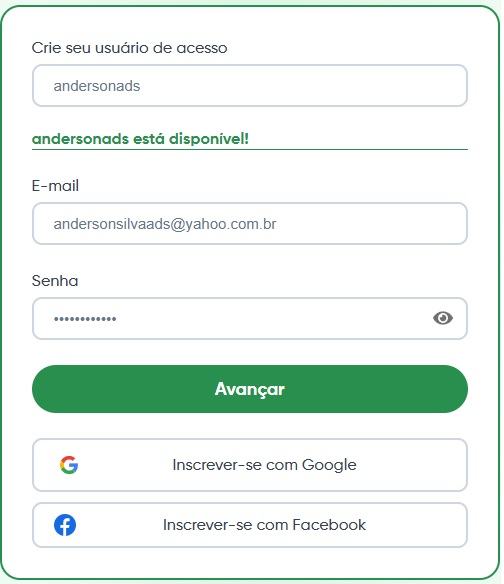
\includegraphics{images/np1/01-bling-cadastro.jpg} 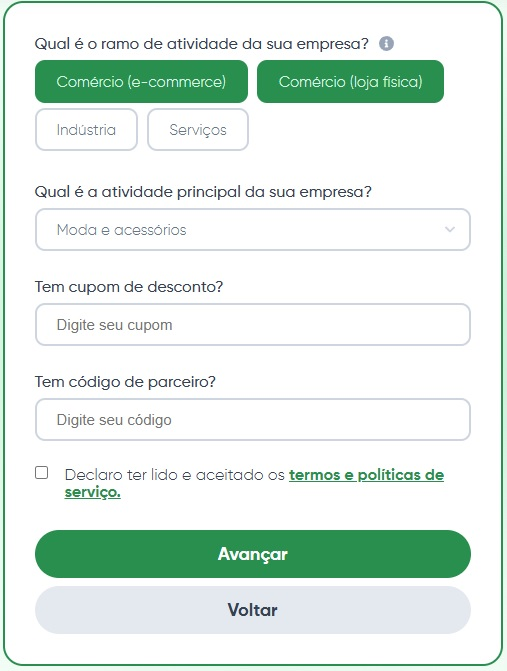
\includegraphics{images/np1/02-bling-selecionar-area-comercial.jpg} 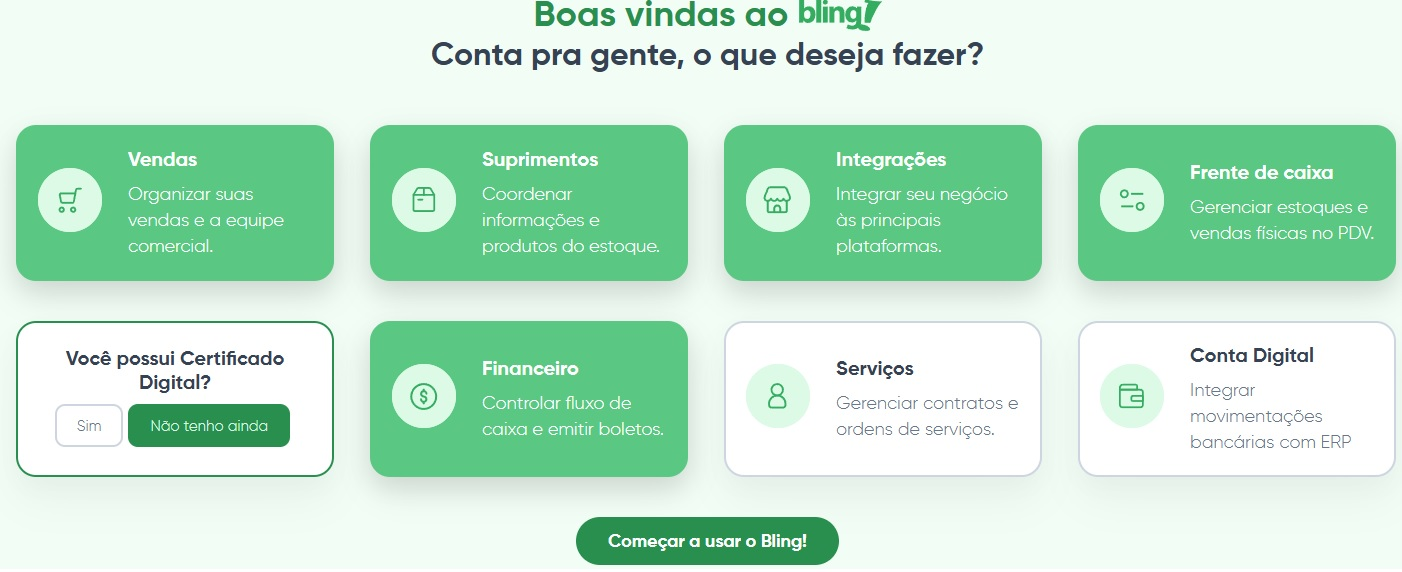
\includegraphics{images/np1/03-bling-escolher-modulos-erp.jpg} 
\includegraphics{images/np1/04-bling-conta-criada.jpg} 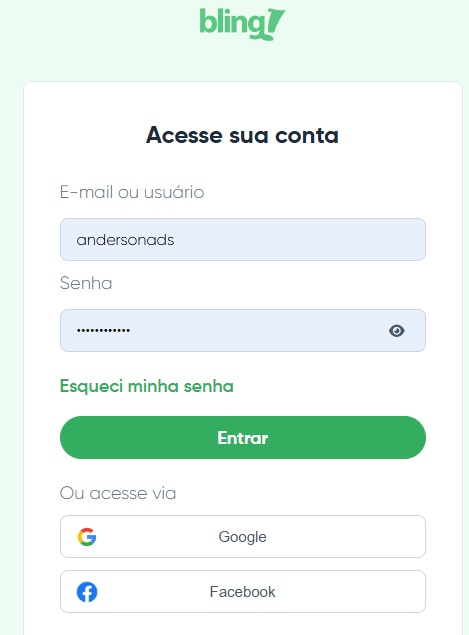
\includegraphics{images/np1/05-bling-logar-usuario-senha.jpg}

\subsubsection{Começar a cadastrar EMPRESA (Conceito de ``Módulo CONTROLE CADASTROS'' dos ERPs)}\label{comeuxe7ar-a-cadastrar-empresa-conceito-de-muxf3dulo-controle-cadastros-dos-erps}

\paragraph{Começar a cadastrar a EMPRESA (pessoa física ou jurídica)}\label{comeuxe7ar-a-cadastrar-a-empresa-pessoa-fuxedsica-ou-juruxeddica}

\includegraphics{images/np1/06-bling-identificar-pessoa-endereço.jpg} 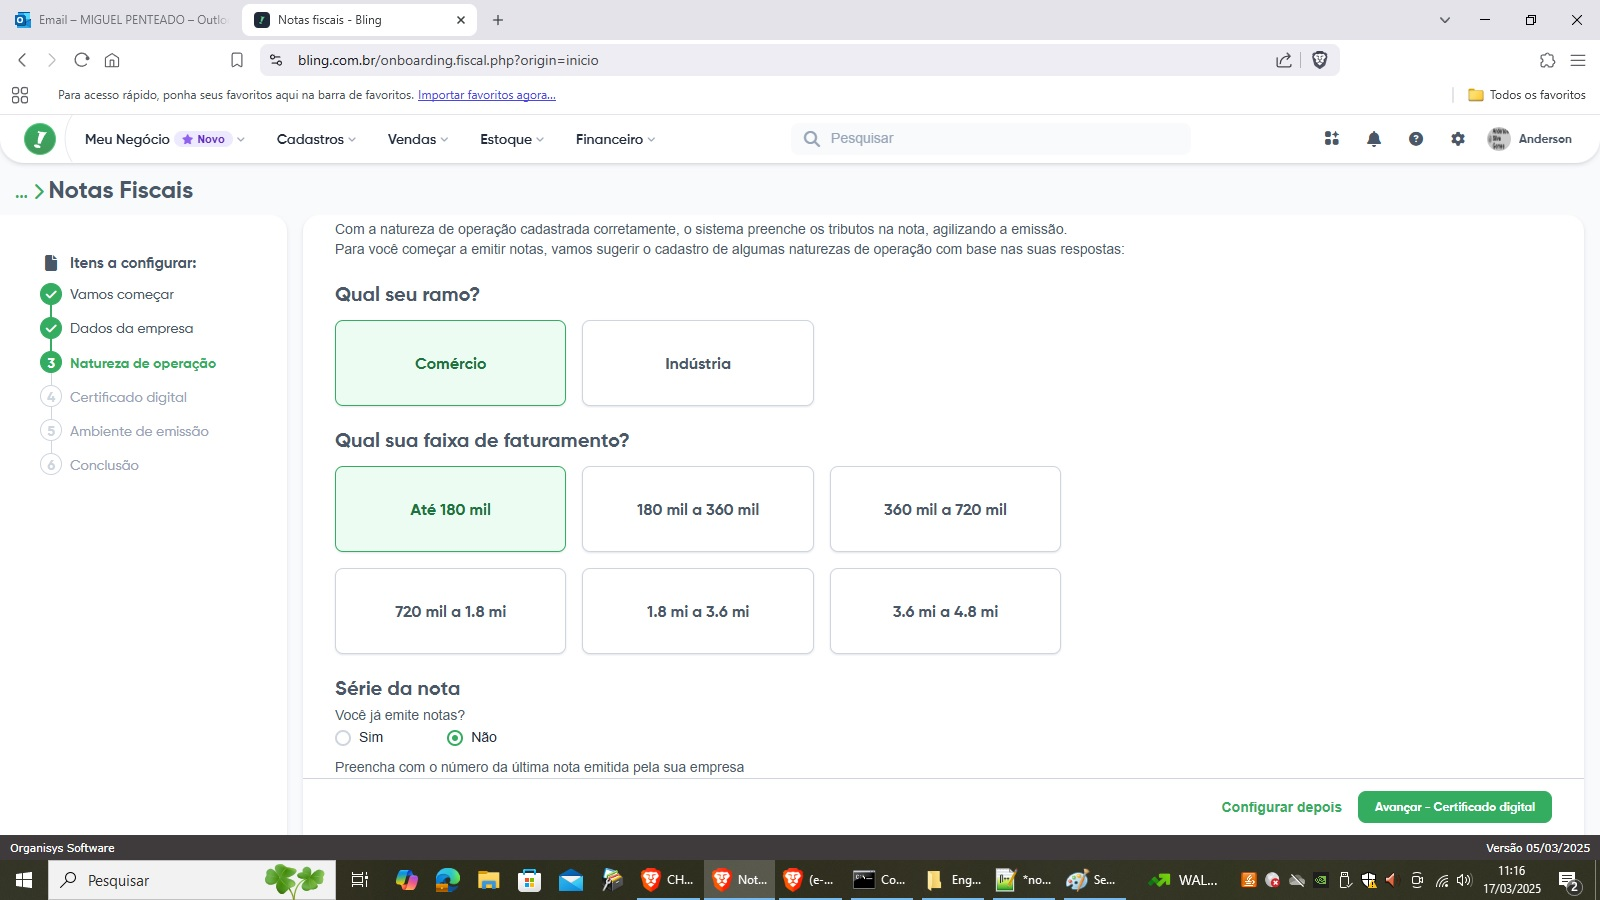
\includegraphics{images/np1/07-bling-natureza-negocio.jpg} 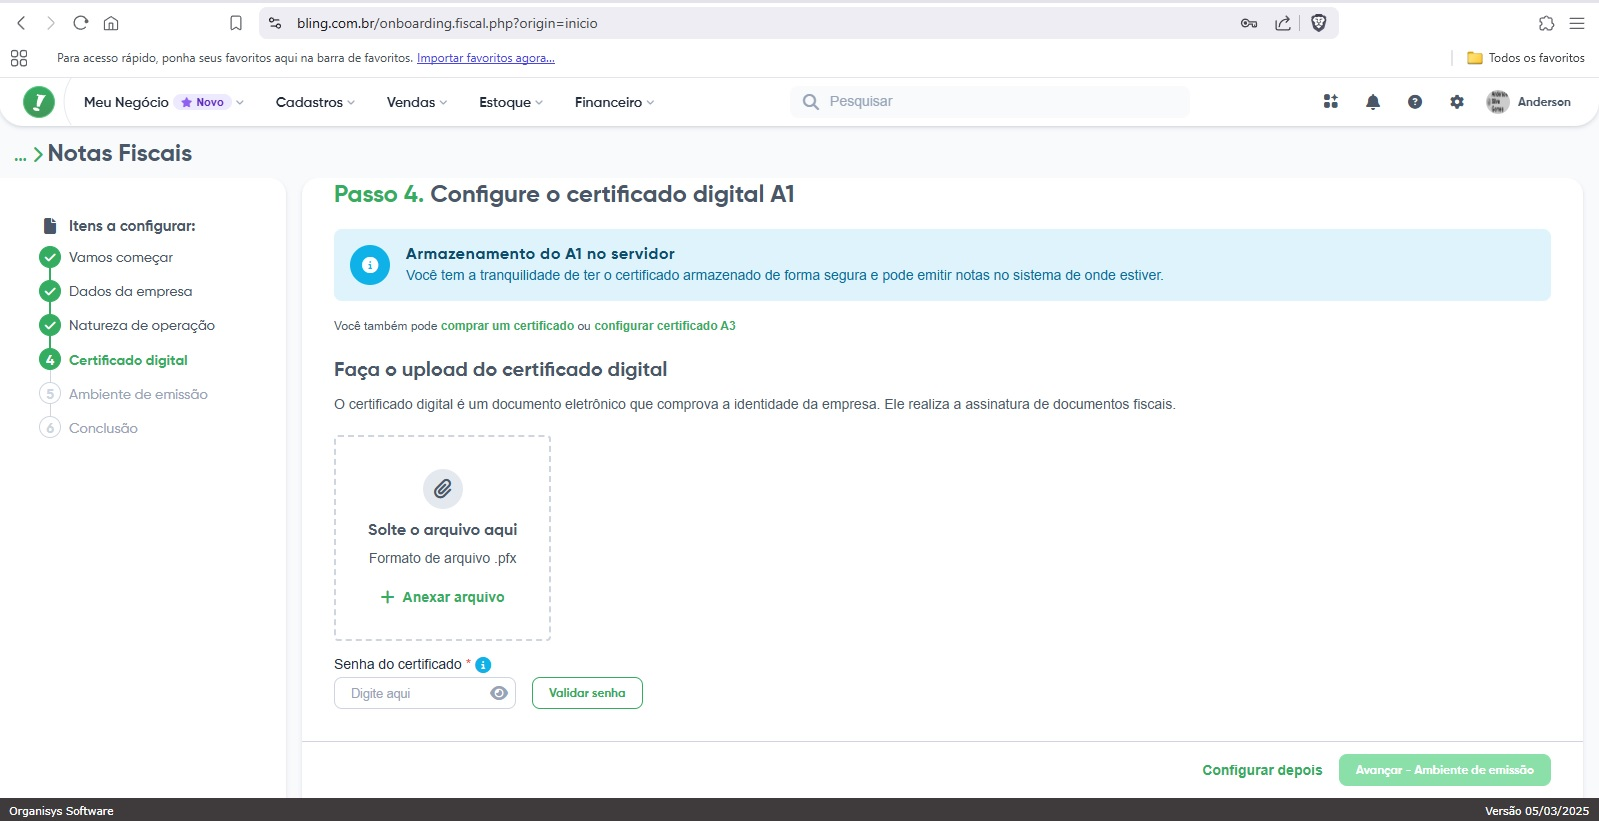
\includegraphics{images/np1/08-bling-certificado-digital-fisco-nota-fiscal.jpg}

\paragraph{Começar a cadastrar as categorias dos produtos (pessoa física ou jurídica)}\label{comeuxe7ar-a-cadastrar-as-categorias-dos-produtos-pessoa-fuxedsica-ou-juruxeddica}

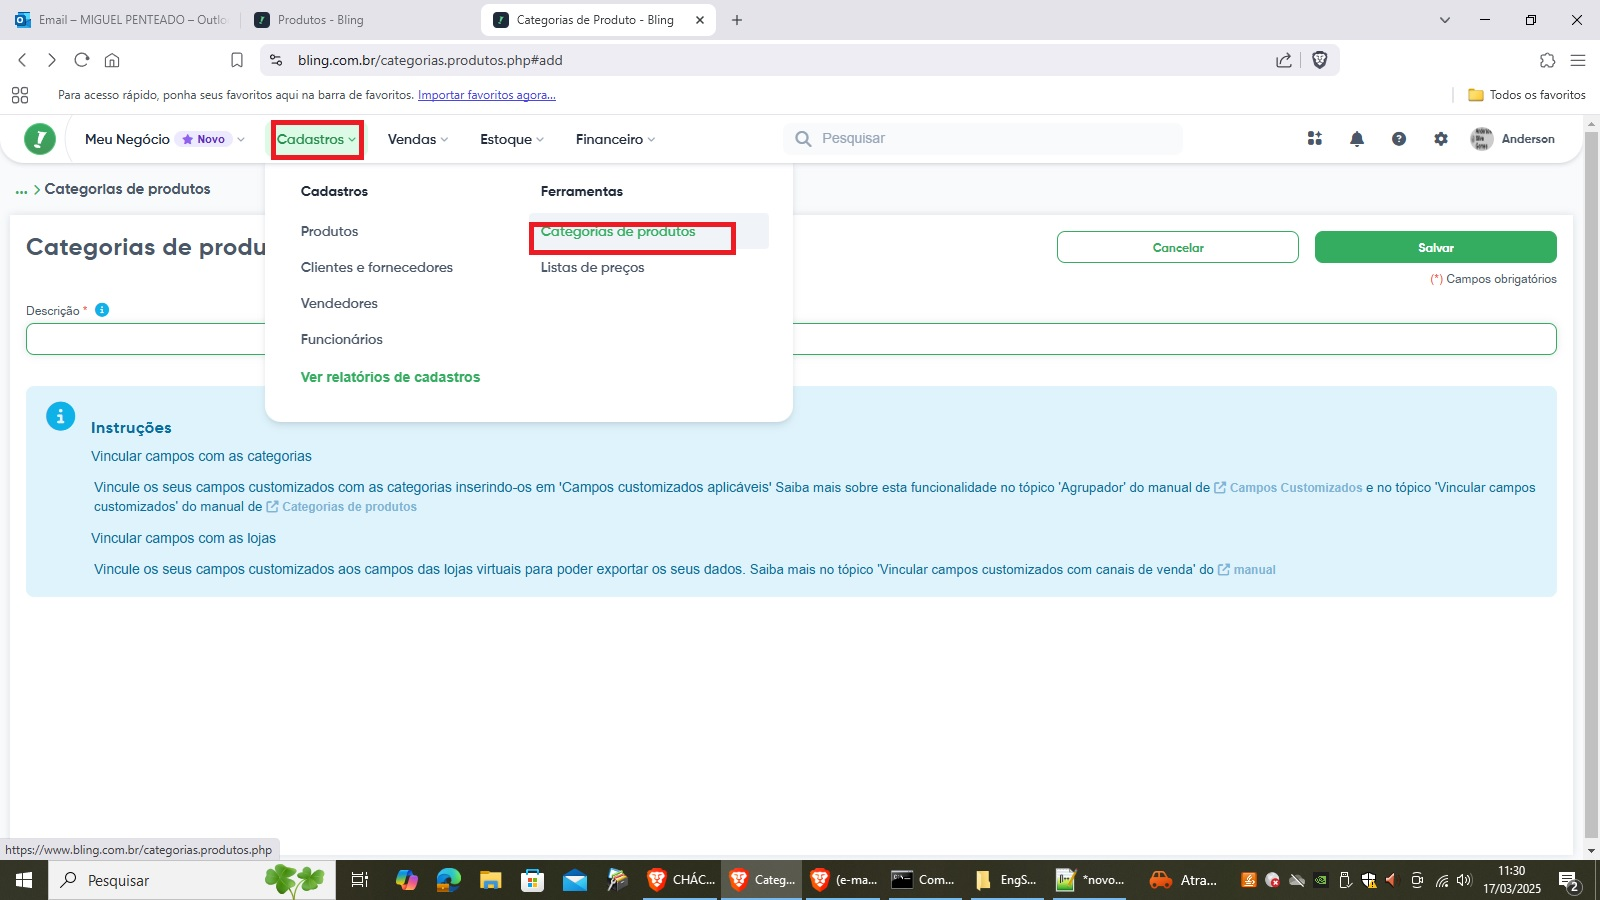
\includegraphics{images/np1/09-bling-cadastrar-categorias-produtos.jpg} 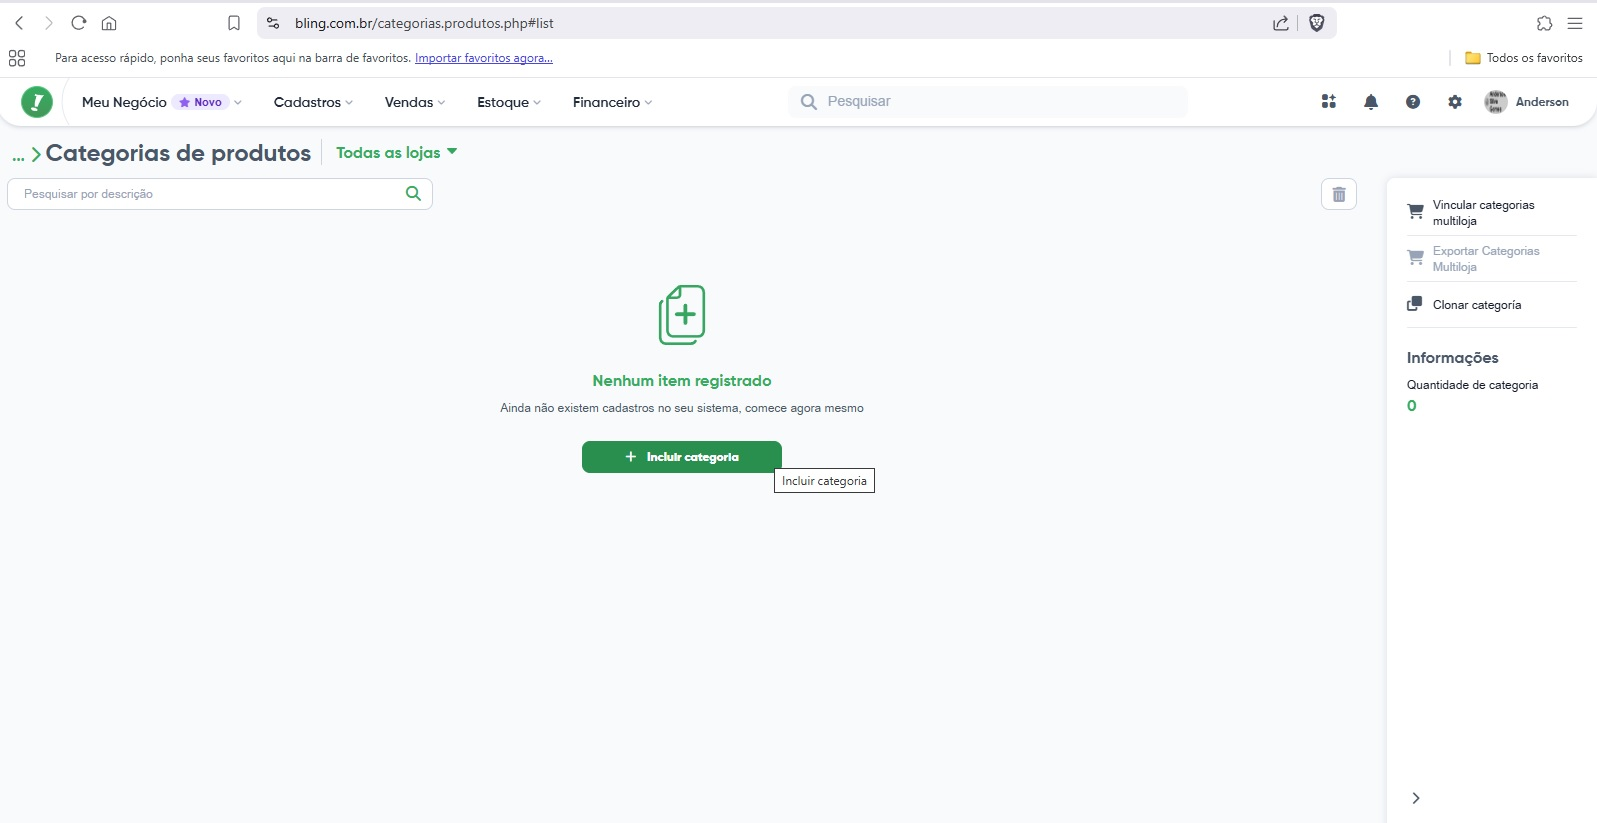
\includegraphics{images/np1/10-bling-cadastrar-categorias-produtos-tela-lista-categorias.jpg} 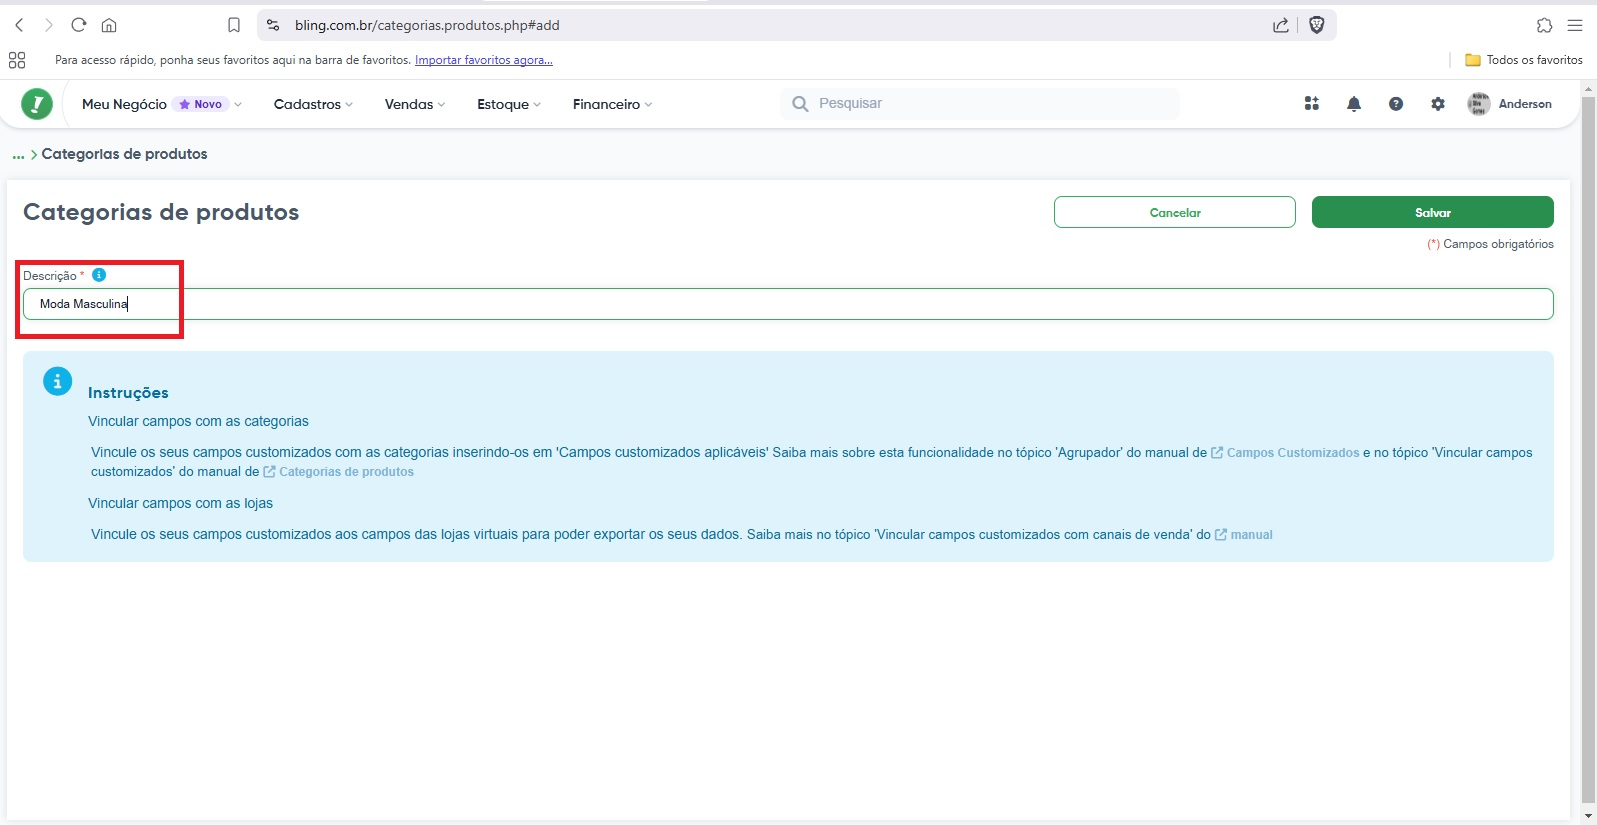
\includegraphics{images/np1/11-bling-cadastrar-moda-masculina.jpg} 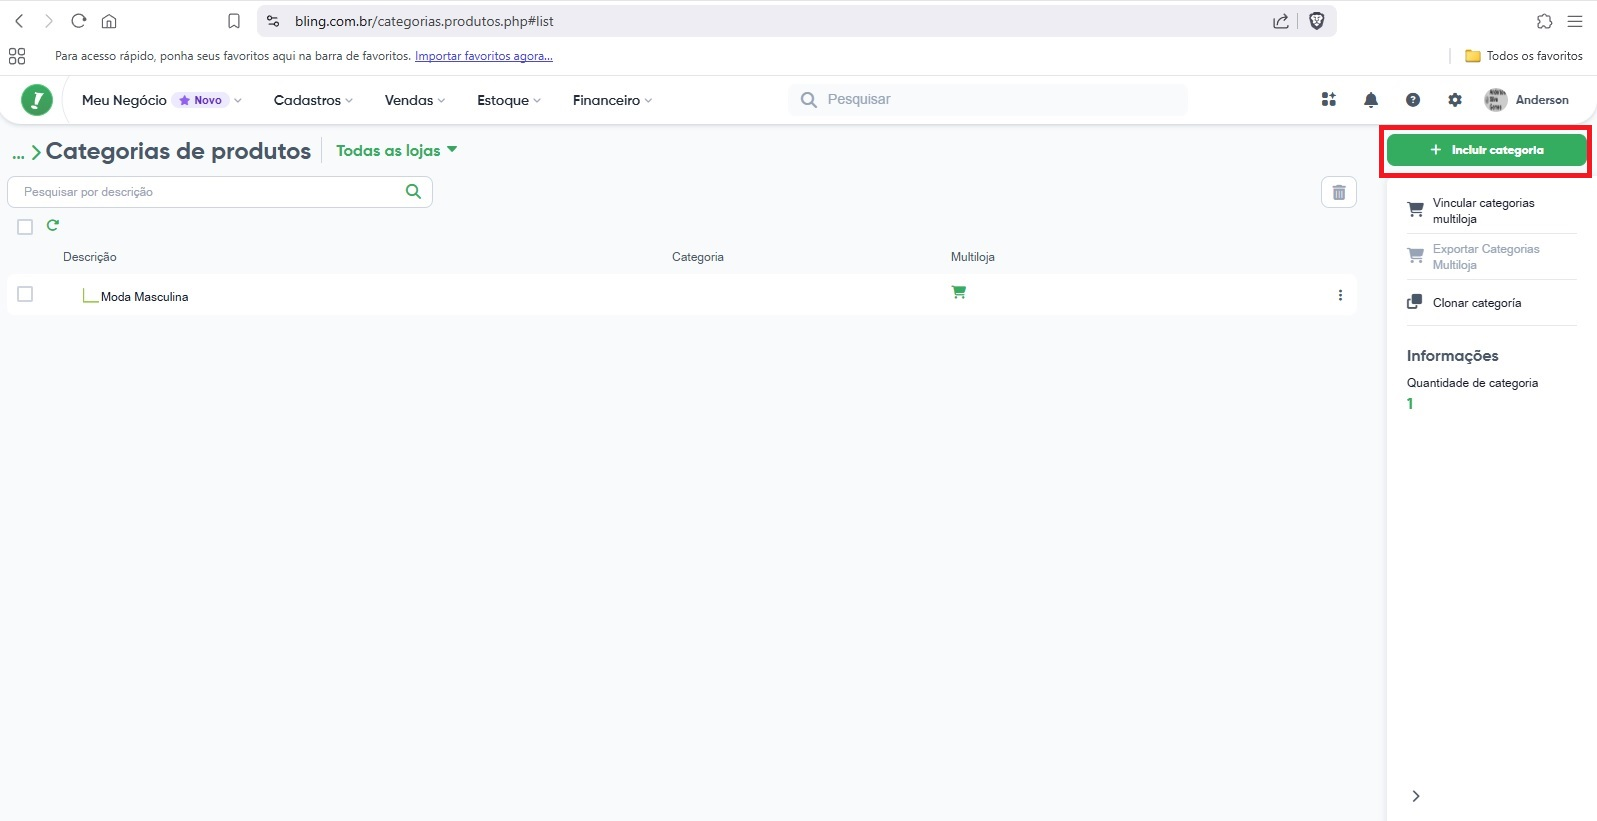
\includegraphics{images/np1/12-bling-cadastrar-categorias-produtos-tela-lista-categorias-inserir-moda-feminina.jpg} 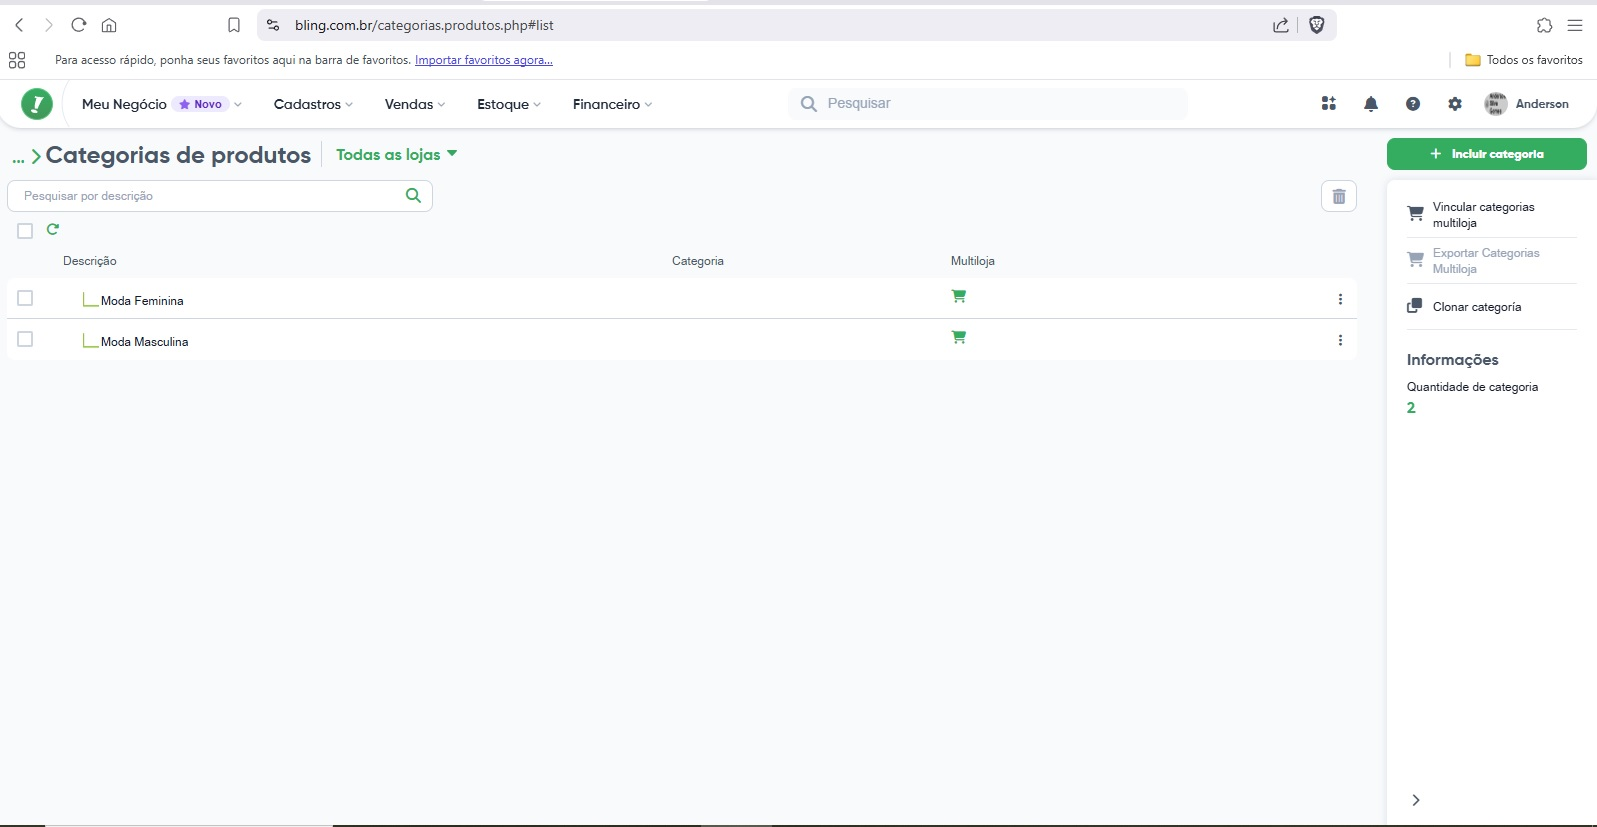
\includegraphics{images/np1/14-bling-cadastrar-subcategoria-moda-masculina-camiseta.jpg} 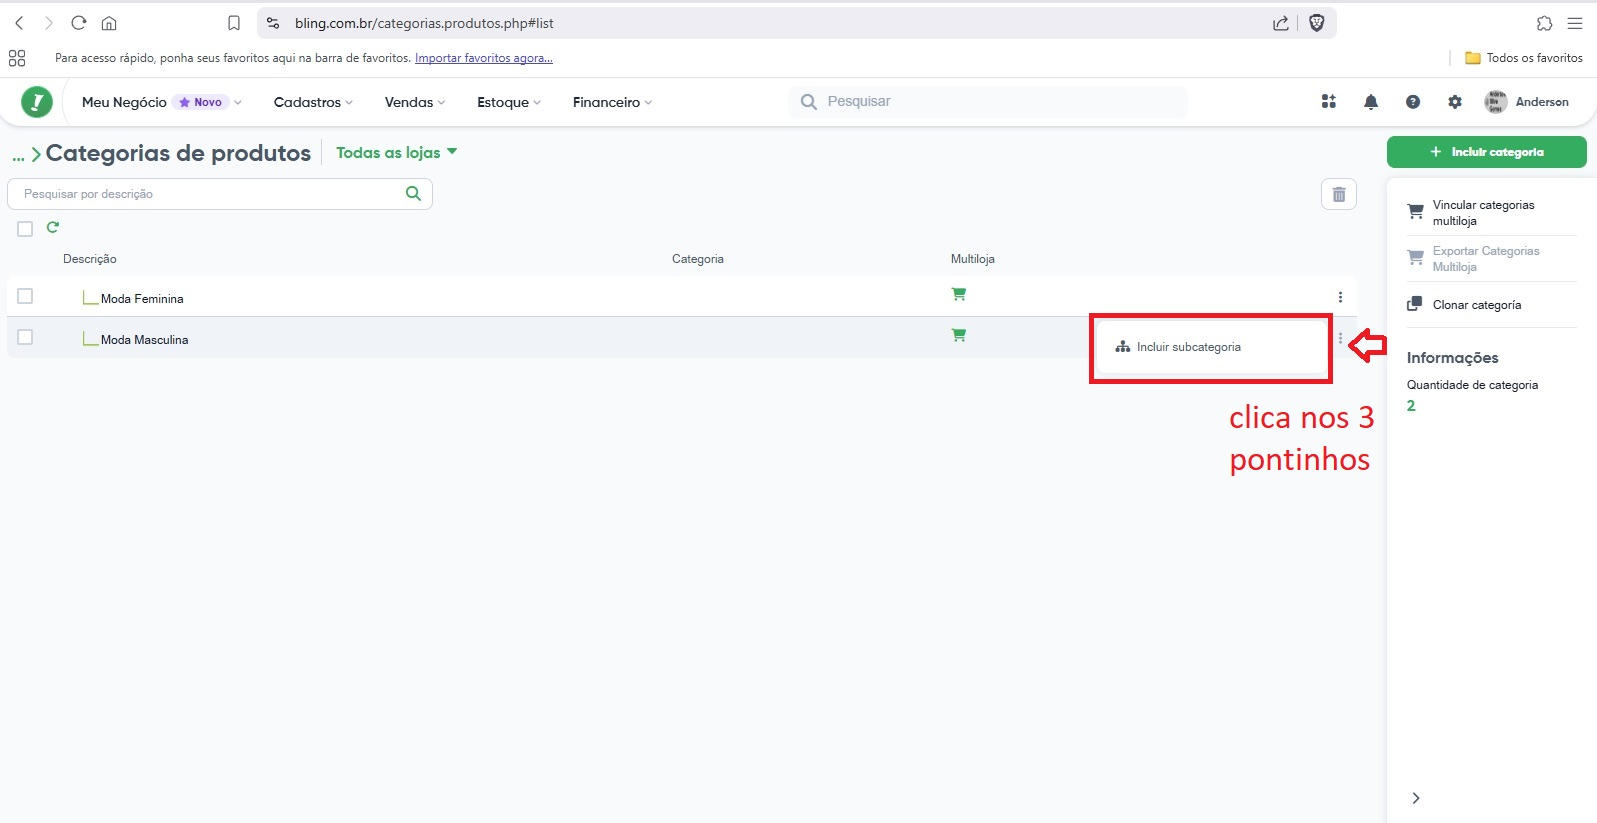
\includegraphics{images/np1/15-bling-cadastrar-subcategoria-moda-masculina-camiseta.jpg} 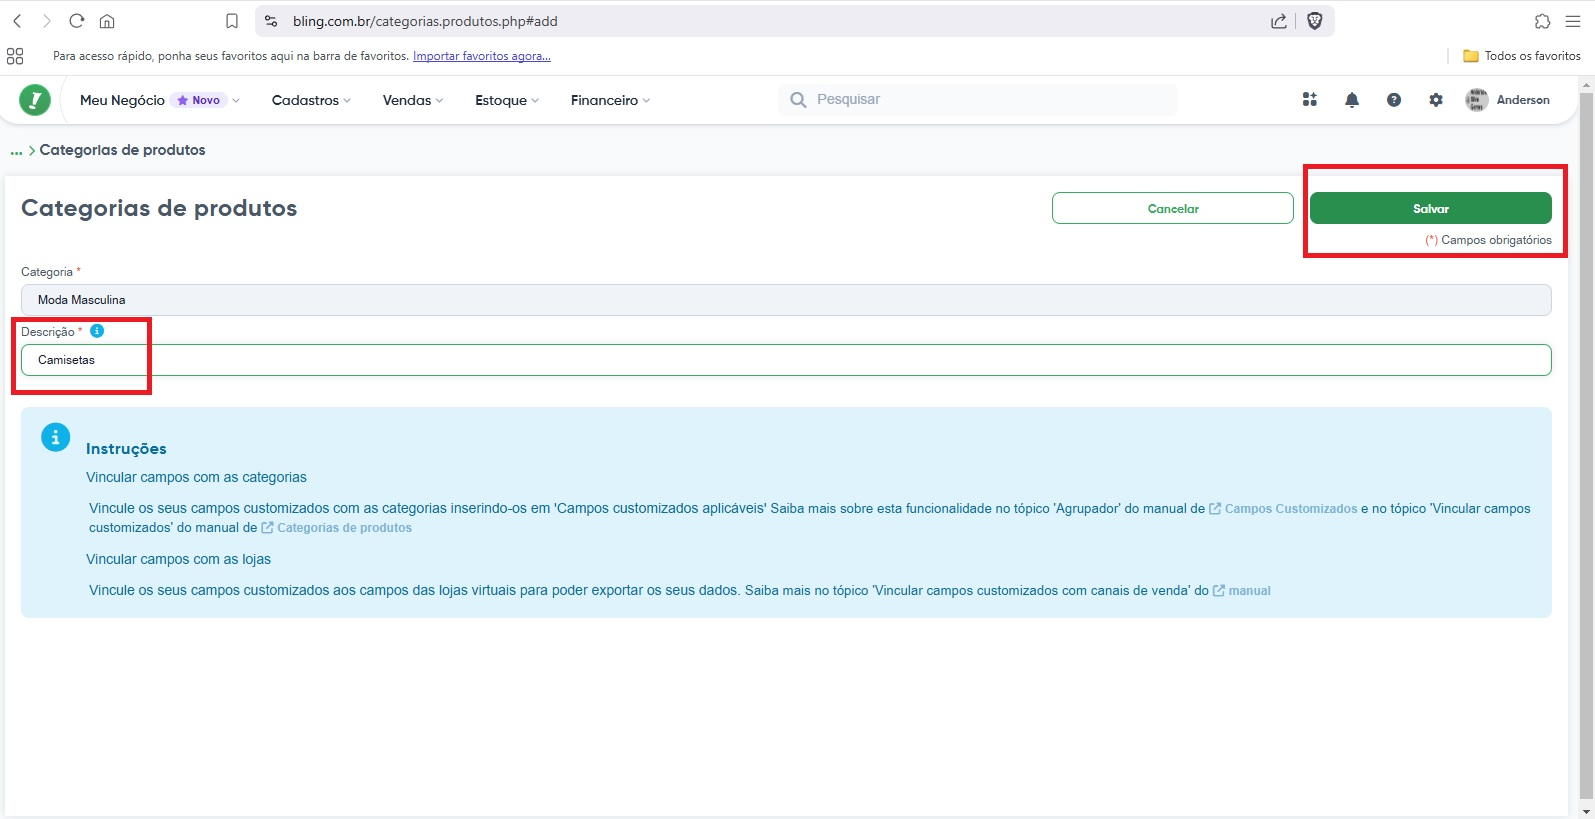
\includegraphics{images/np1/16-bling-confirmar-cadastro-camisetas-em-moda-masculina.jpg} 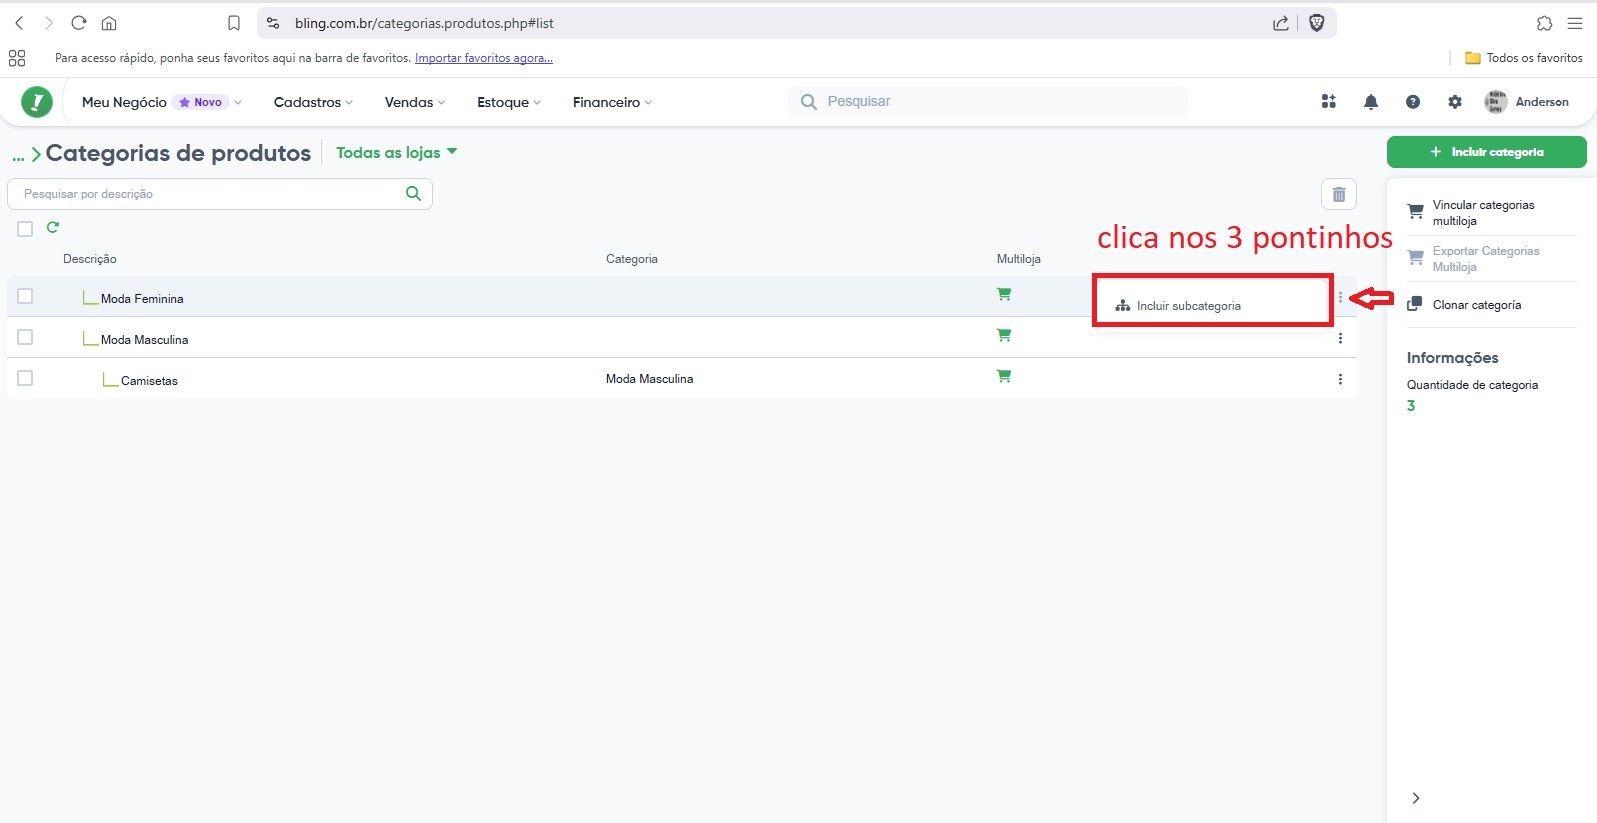
\includegraphics{images/np1/17-bling-cadastrar-subcategoria-moda-feminina-vestido.jpg} 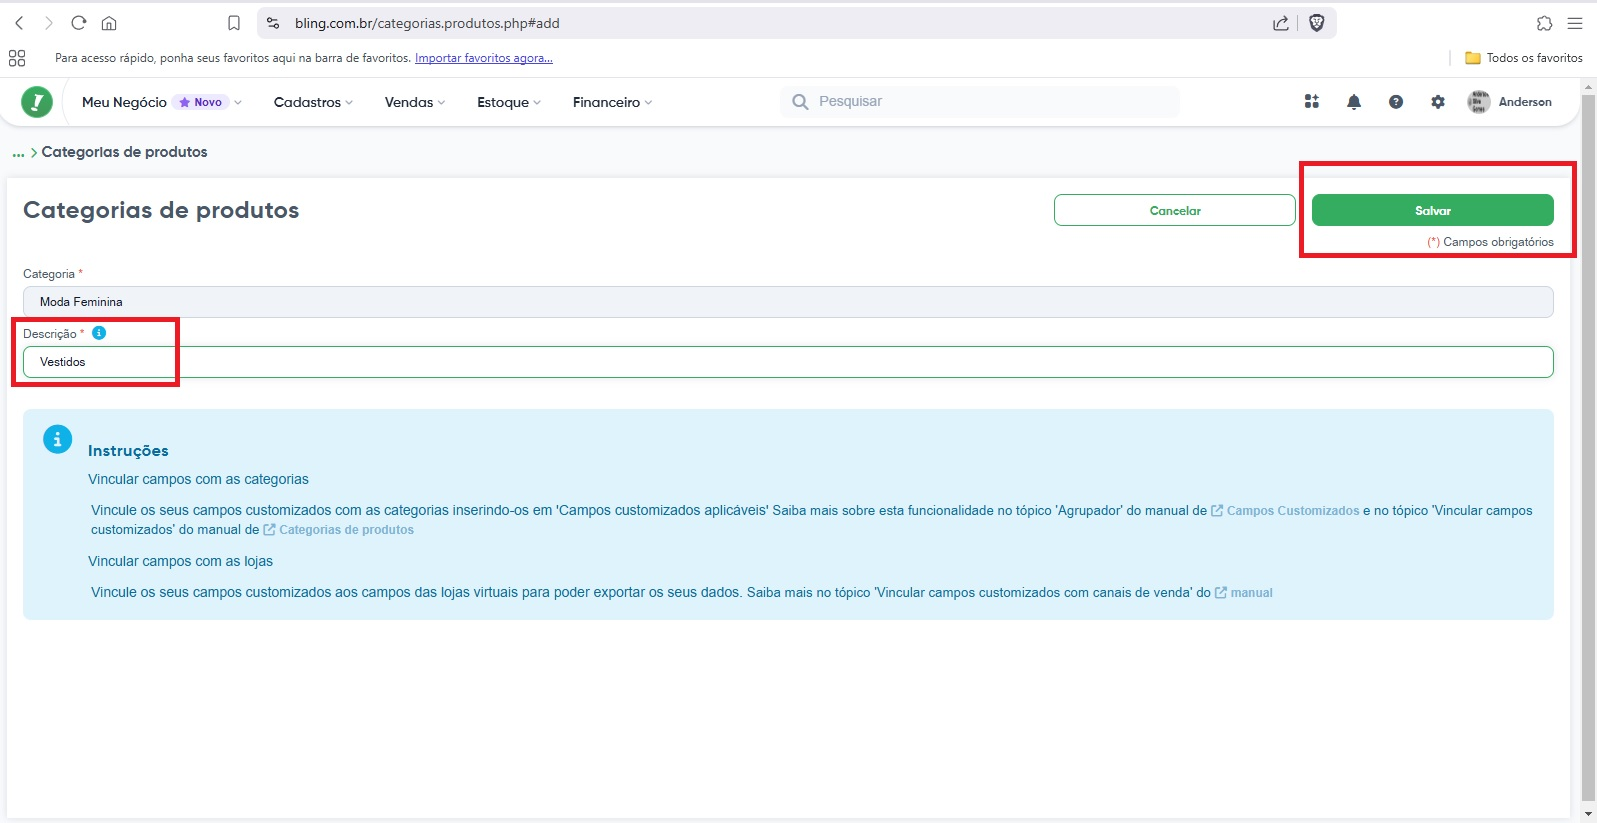
\includegraphics{images/np1/18-bling-confirmar-cadastro-vestidos-em-moda-feminina.jpg} 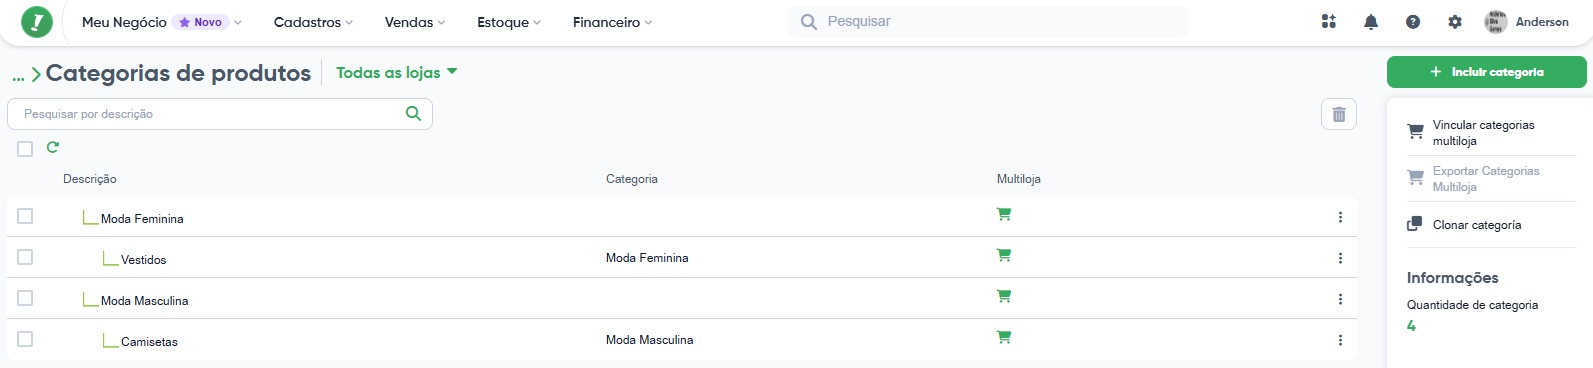
\includegraphics{images/np1/19-categorias-cadastradas.jpg}

\paragraph{Começar a cadastrar os produtos (pessoa física ou jurídica)}\label{comeuxe7ar-a-cadastrar-os-produtos-pessoa-fuxedsica-ou-juruxeddica}

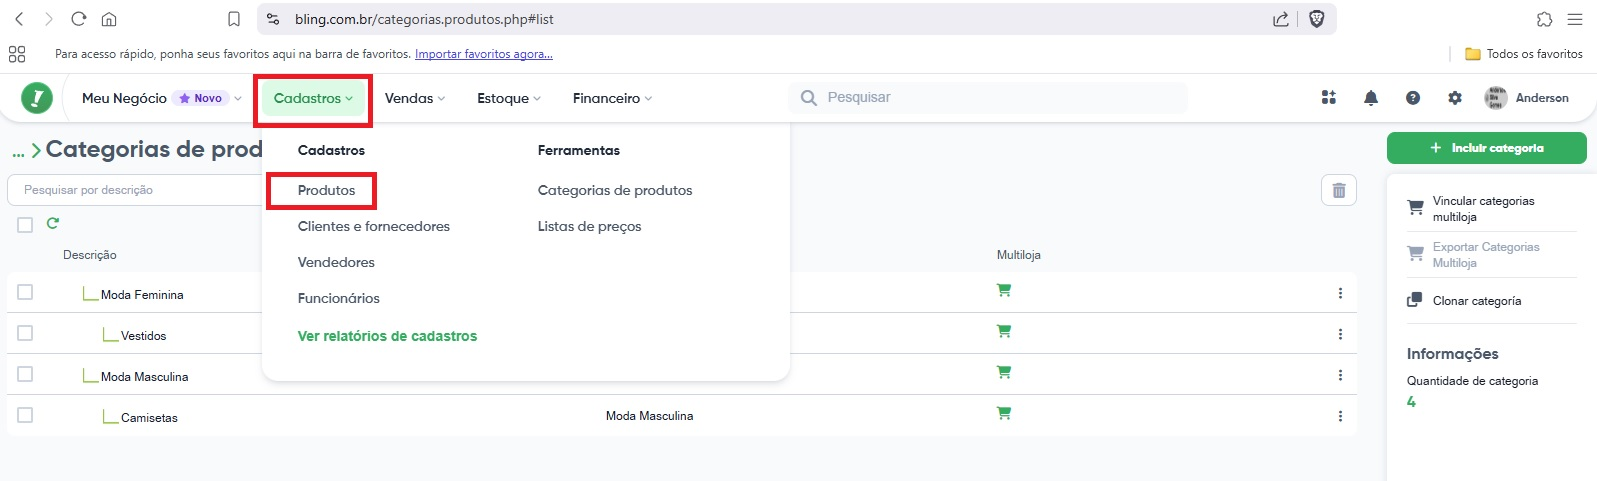
\includegraphics{images/np1/20-cadastrar-produtos.jpg} 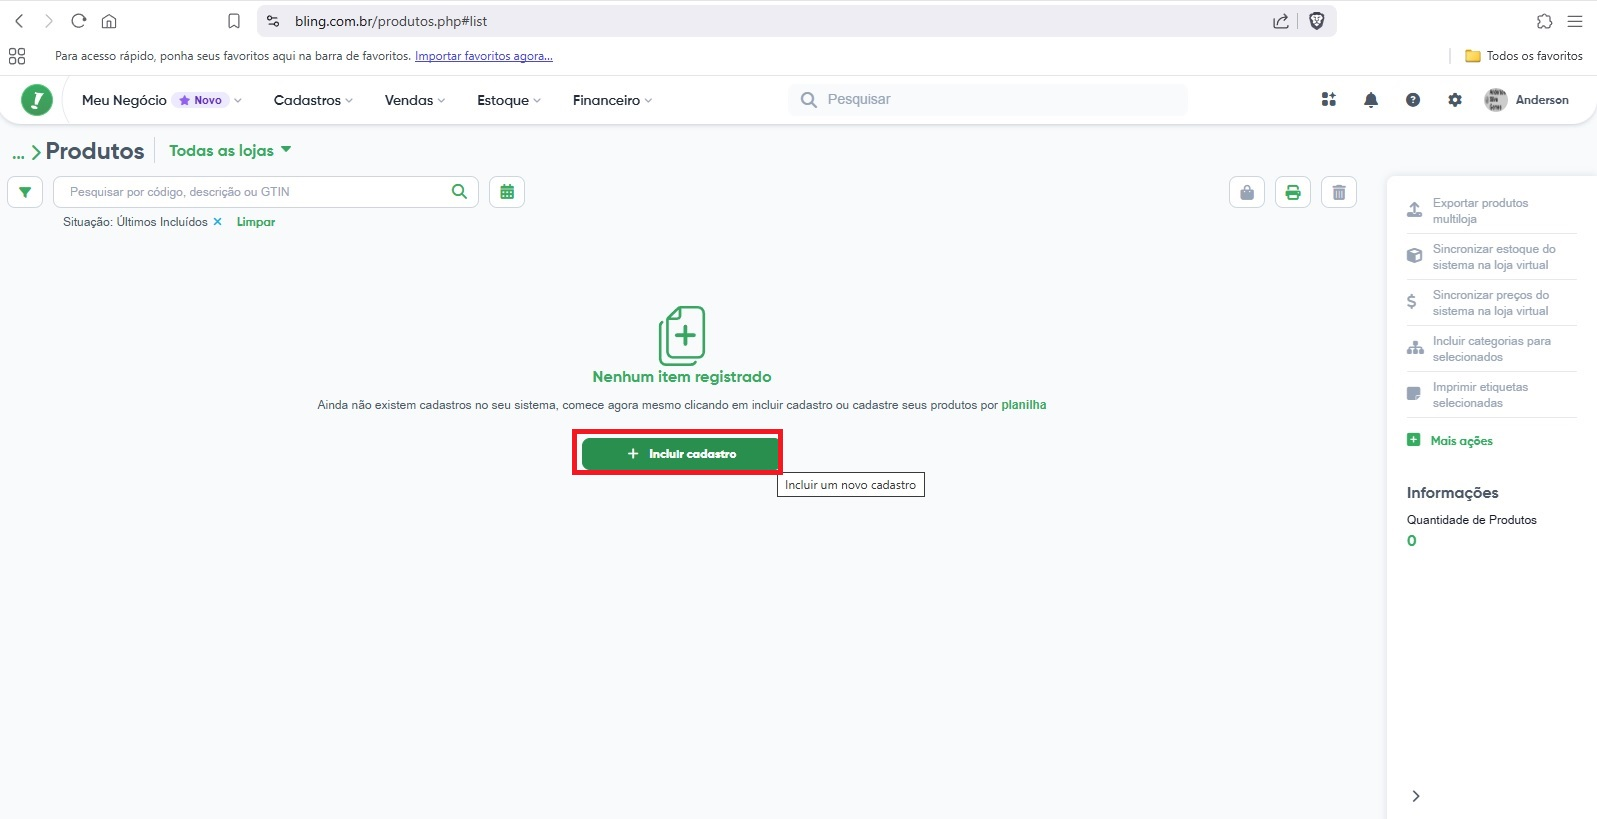
\includegraphics{images/np1/21-cadastro-produtos-inserir-produto.jpg} 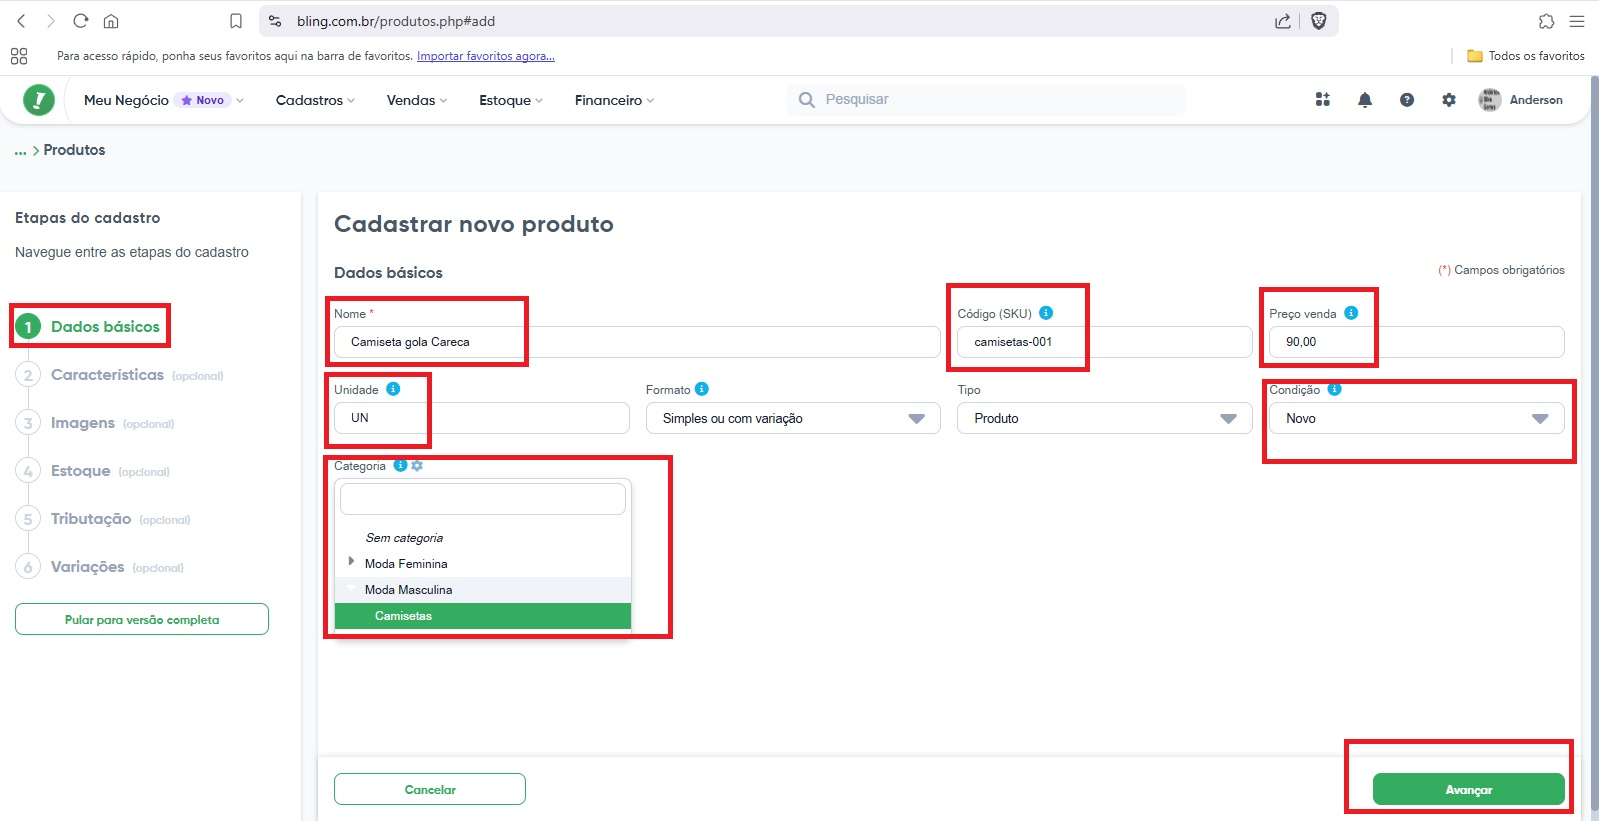
\includegraphics{images/np1/22-cadastro-produtos-inserir-produto-dados-basicos.jpg} 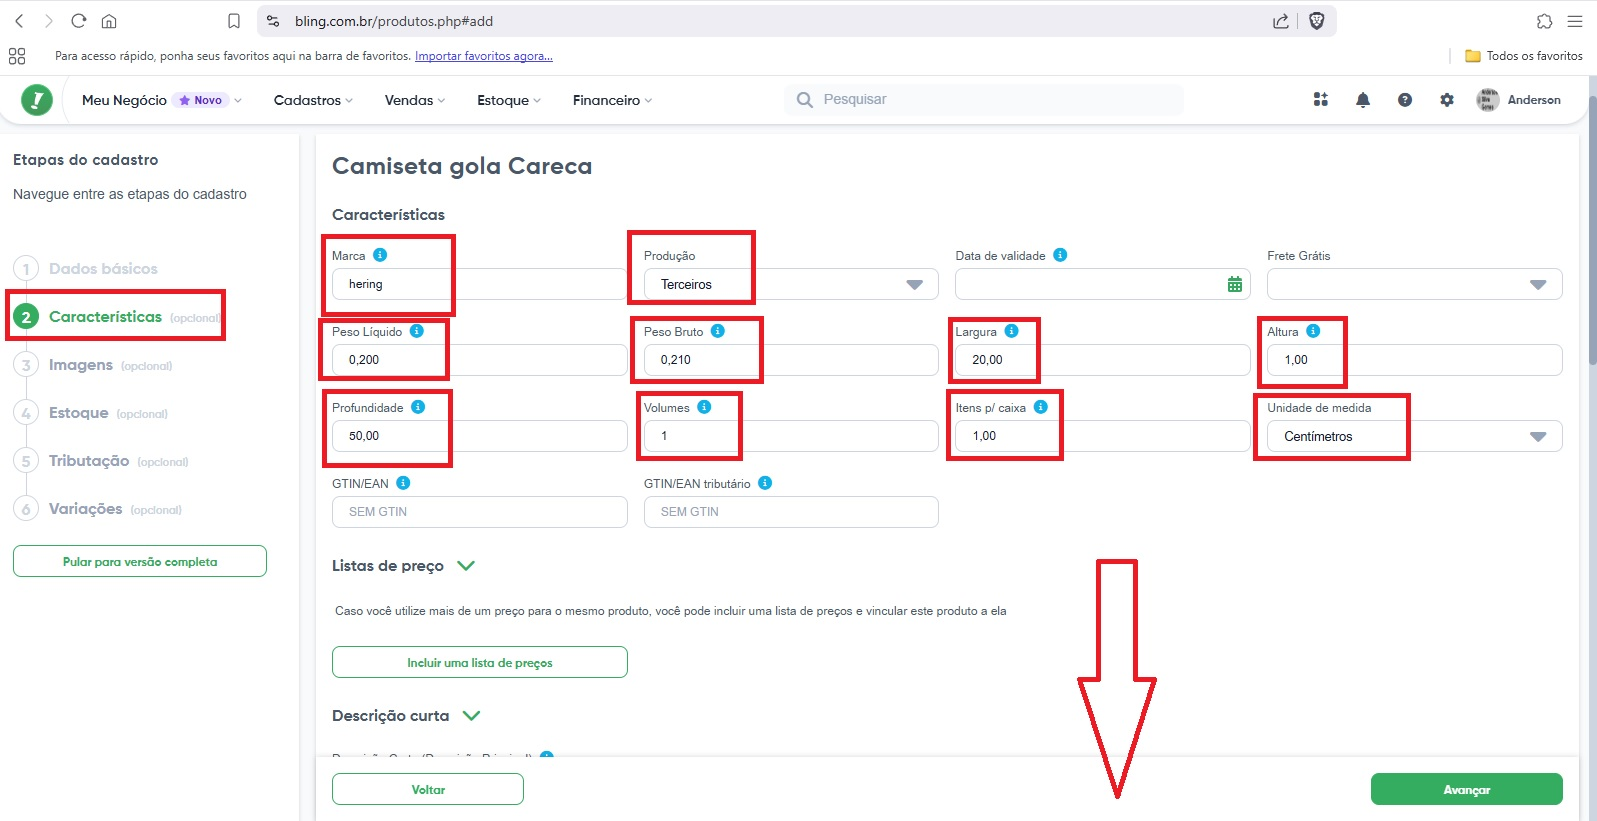
\includegraphics{images/np1/23-cadastro-produtos-inserir-detalhes-e-commerce.jpg} 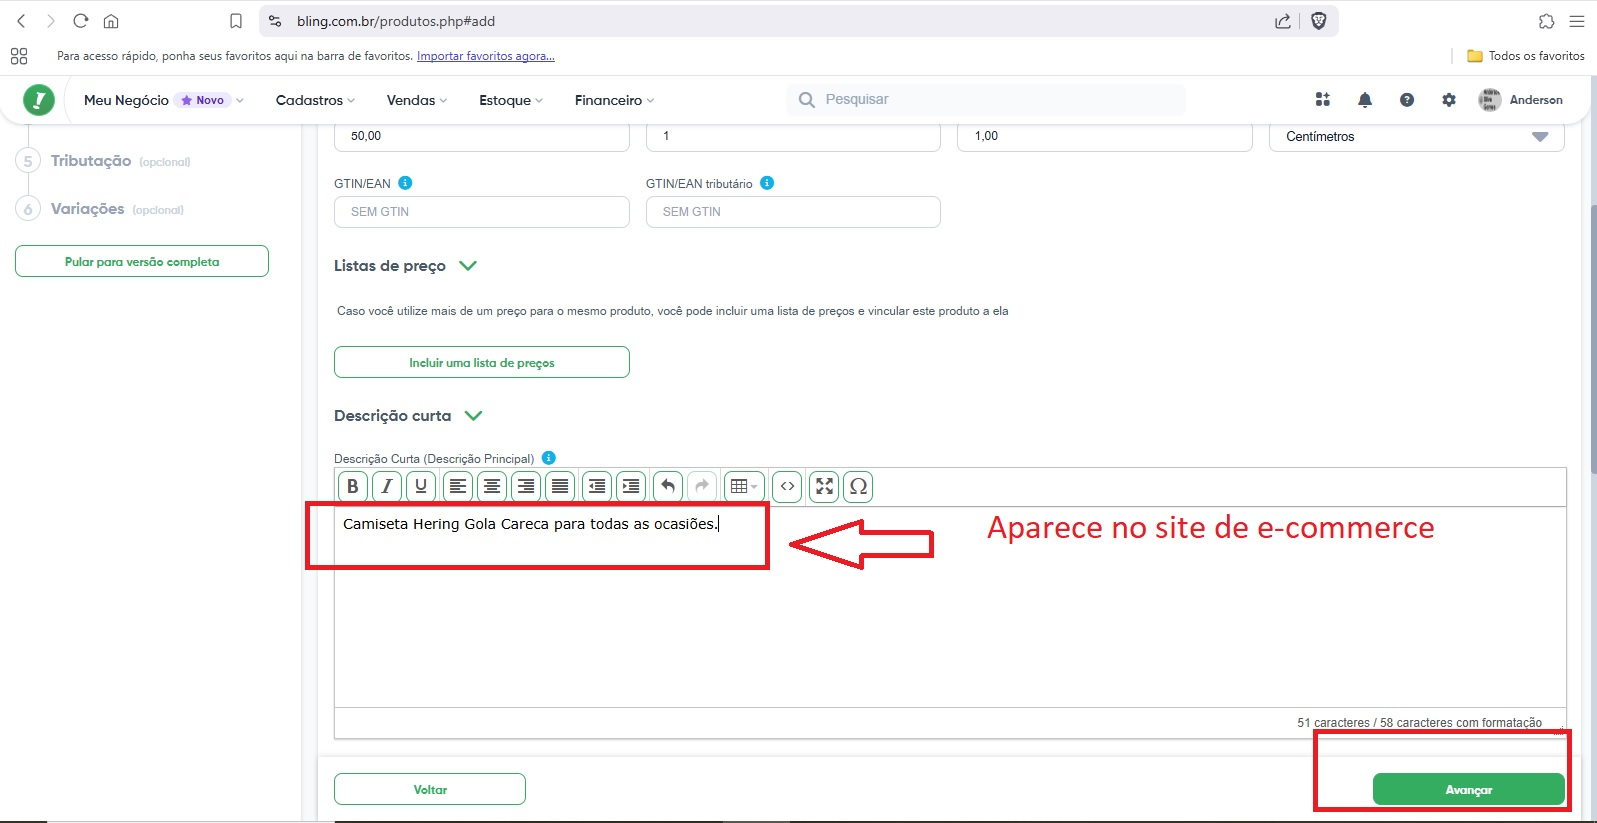
\includegraphics{images/np1/24-cadastro-produtos-inserir-detalhes-e-commerce-descricao.jpg} 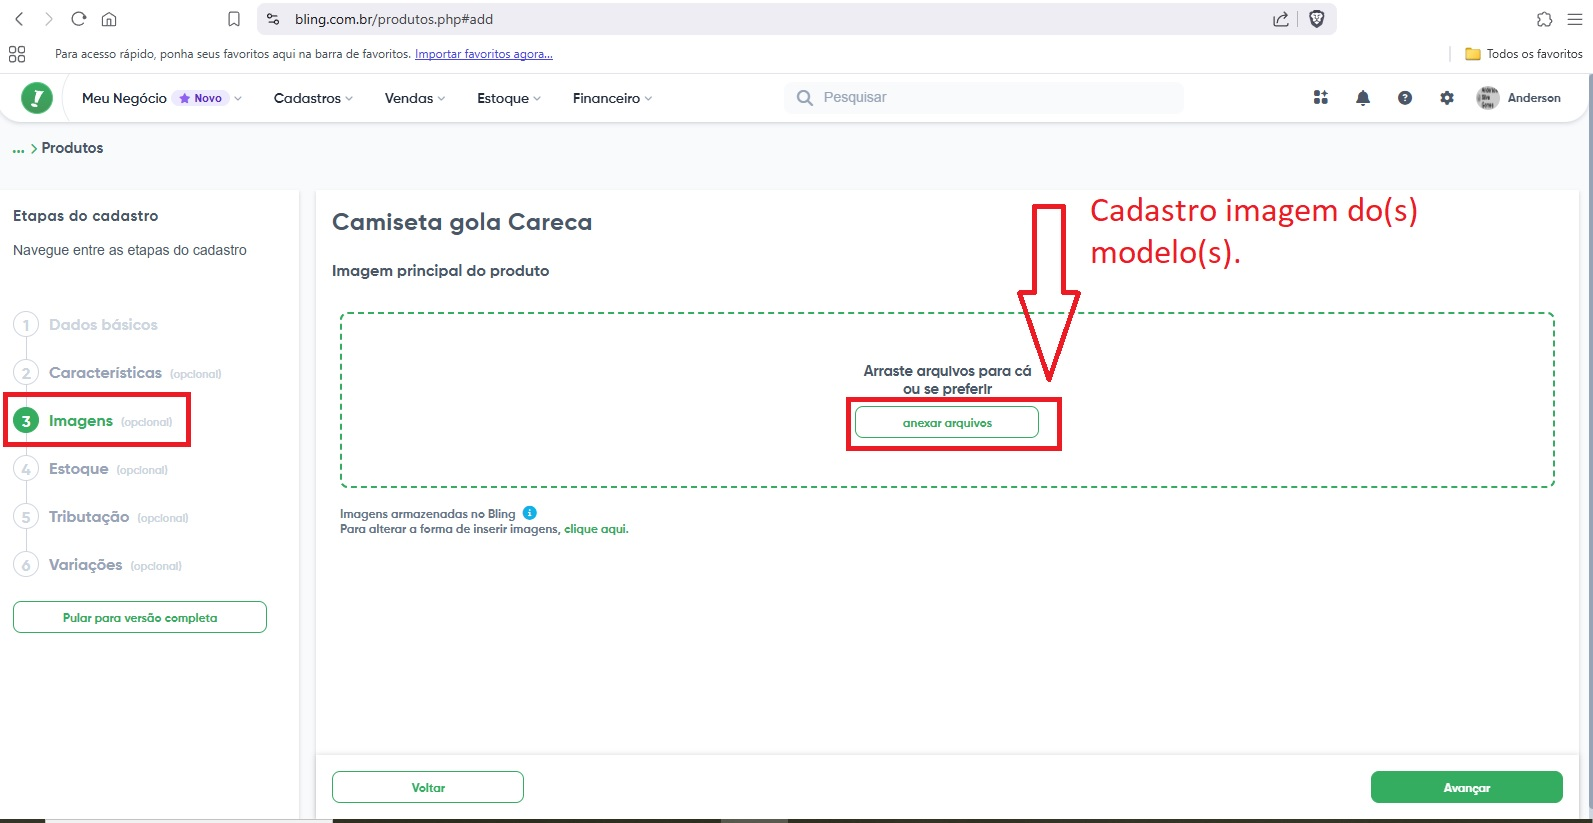
\includegraphics{images/np1/25-cadastro-produtos-inserir-imagem-produtos.jpg} 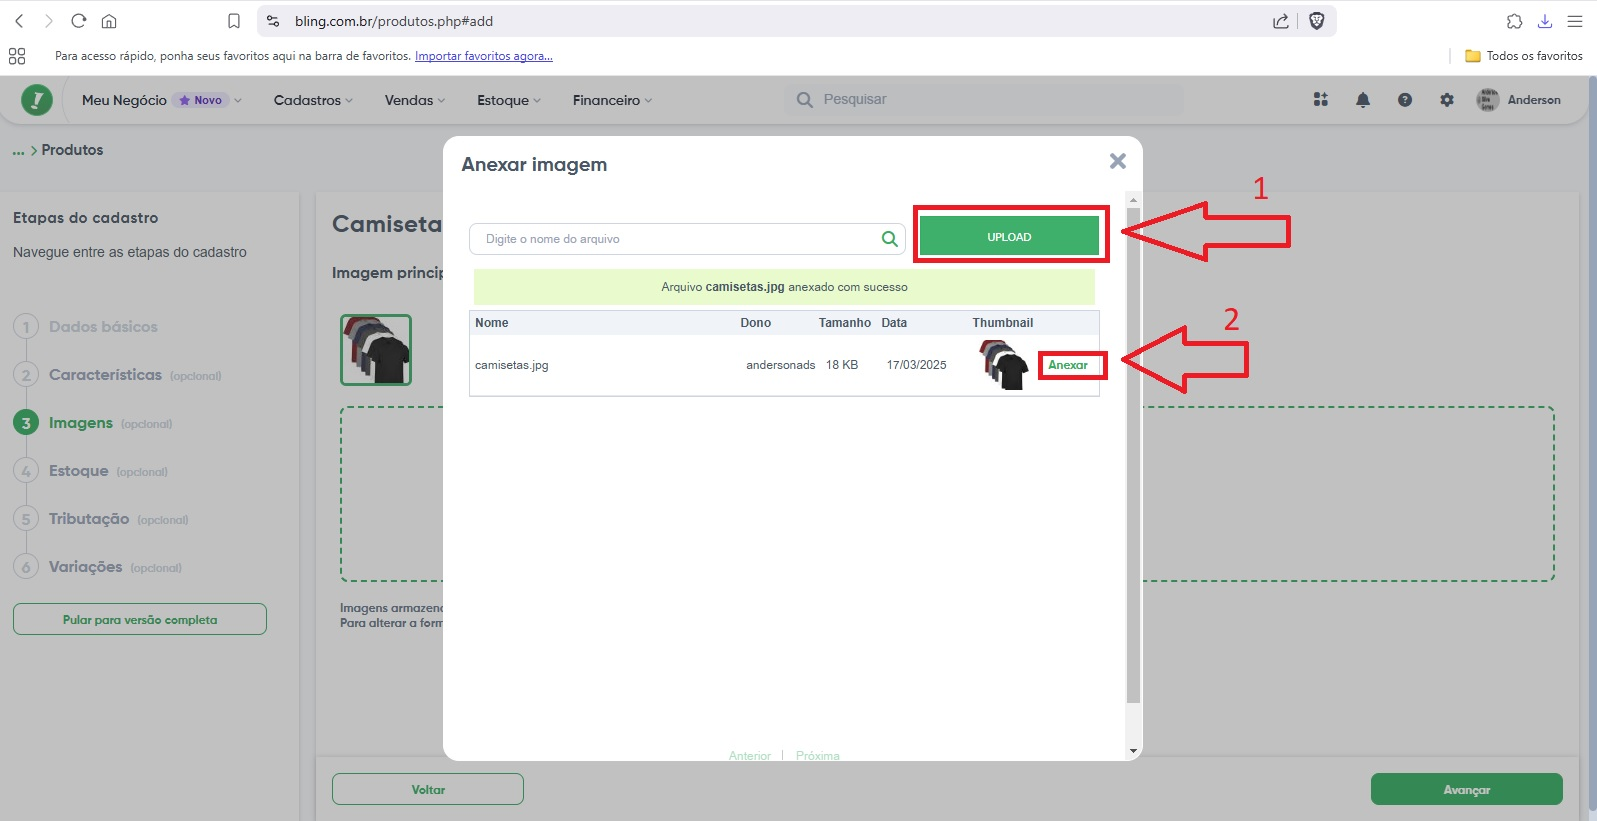
\includegraphics{images/np1/26-cadastro-produtos-inserir-imagem-produtos.jpg} 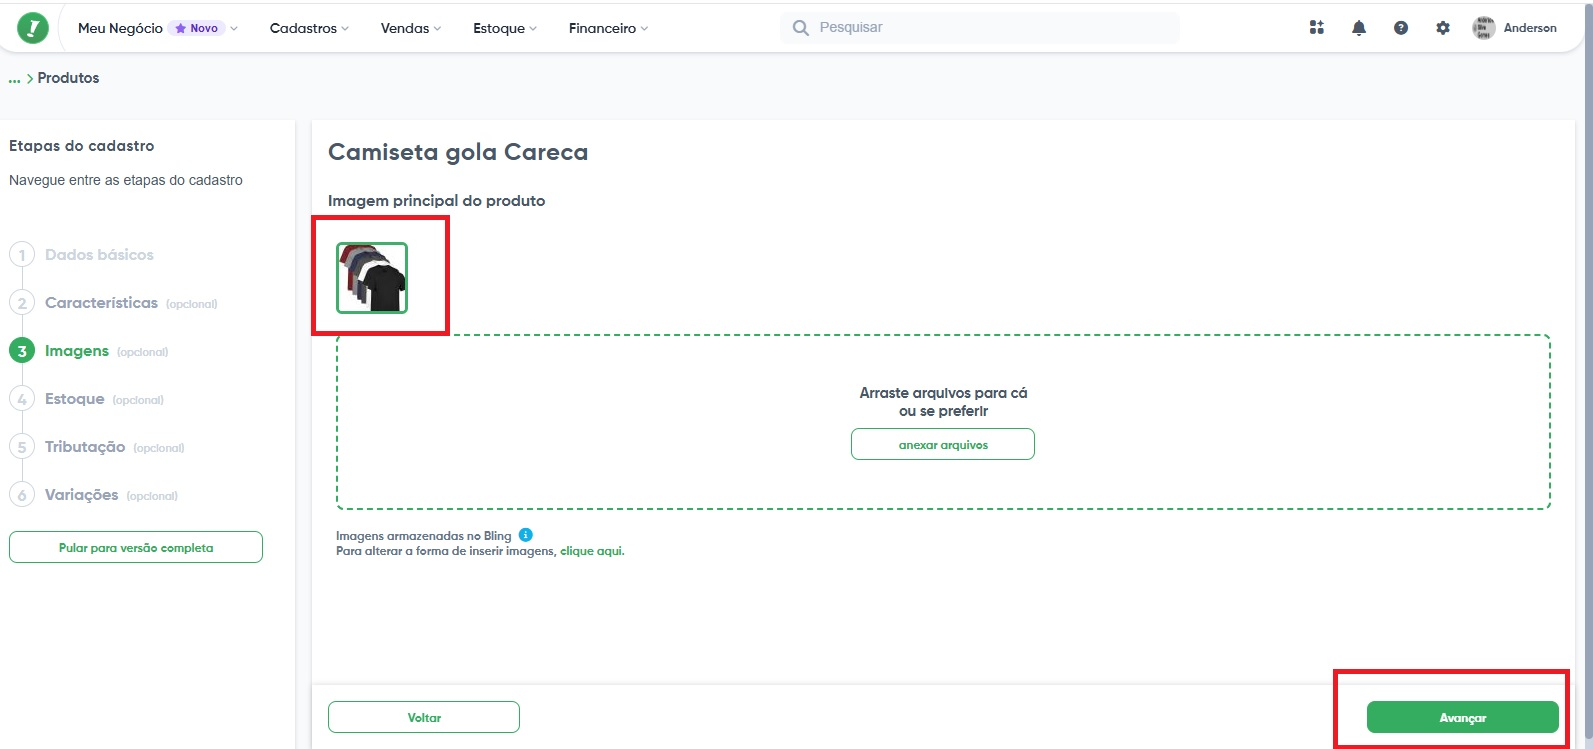
\includegraphics{images/np1/27-cadastro-produtos-inserir-imagem-produtos-cadastradas.jpg} 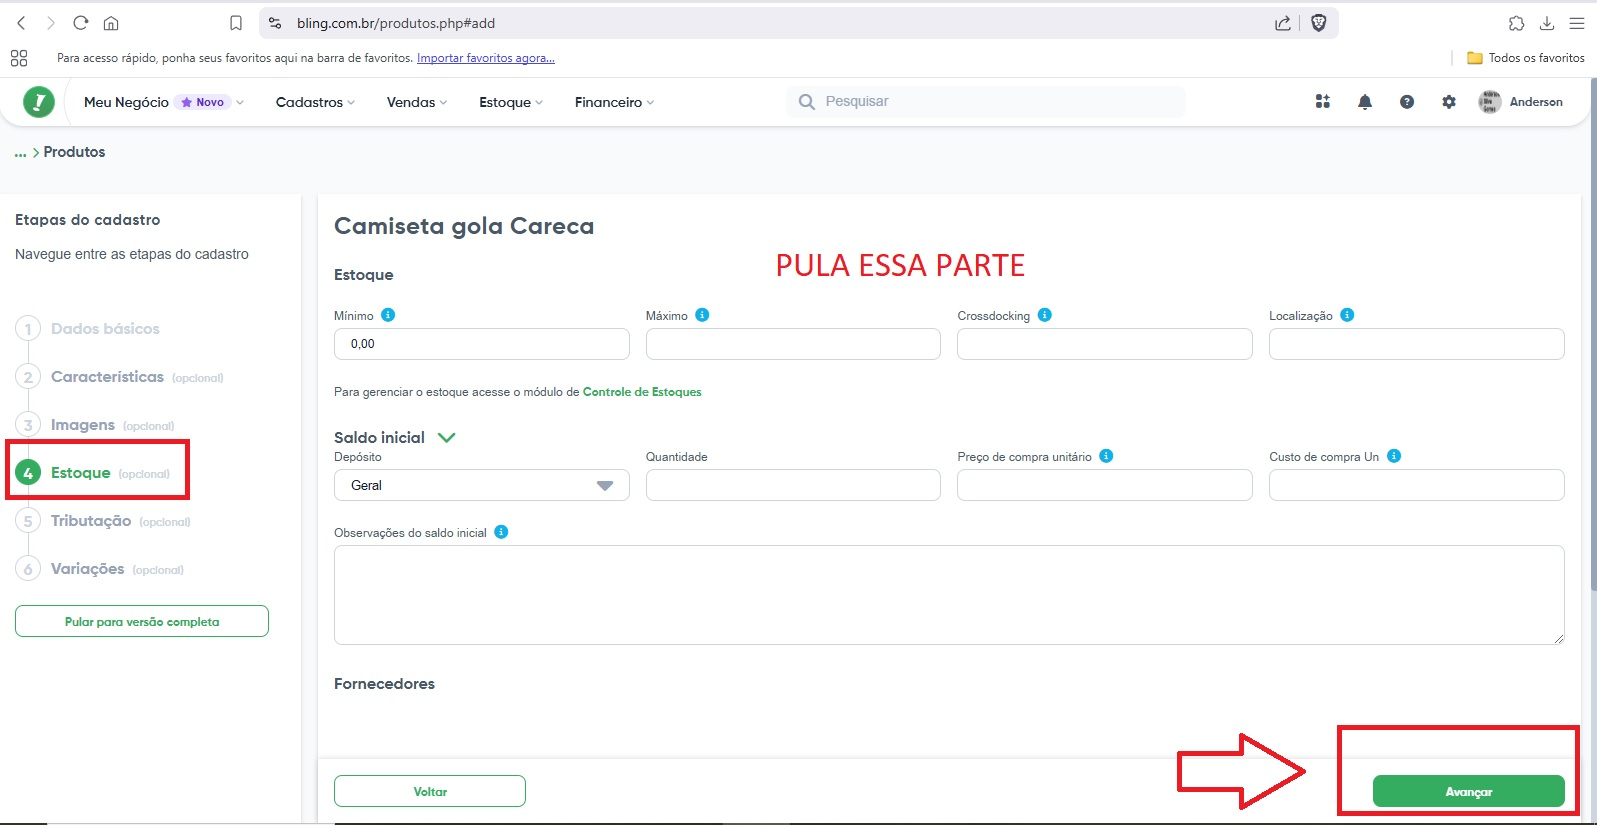
\includegraphics{images/np1/28-cadastro-produtos-quantidade-estoque.jpg} 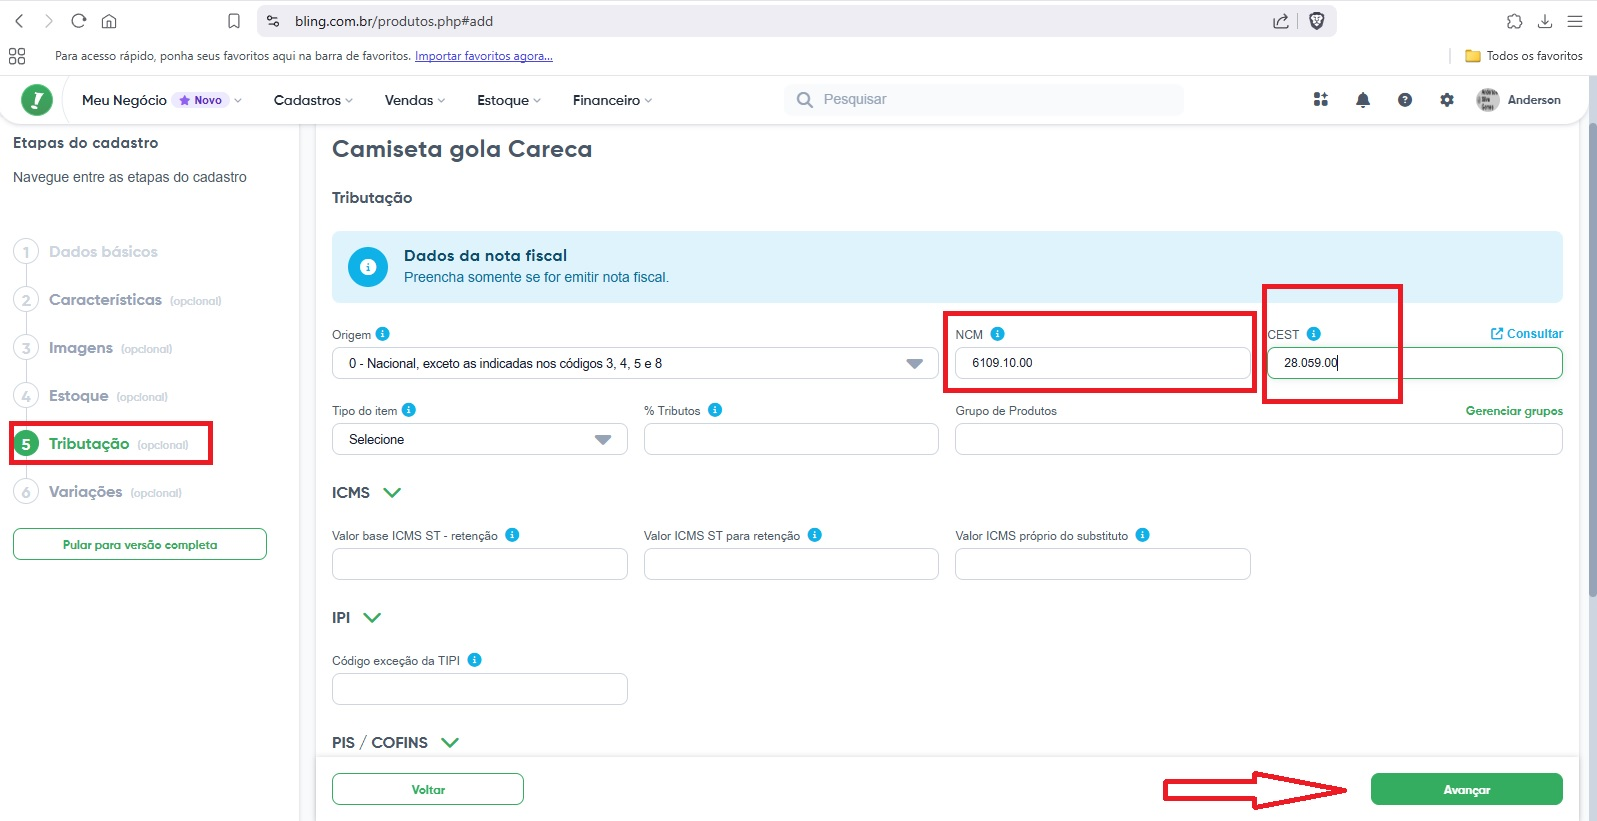
\includegraphics{images/np1/29-cadastro-produtos-fiscal-NCM-CEST.jpg} 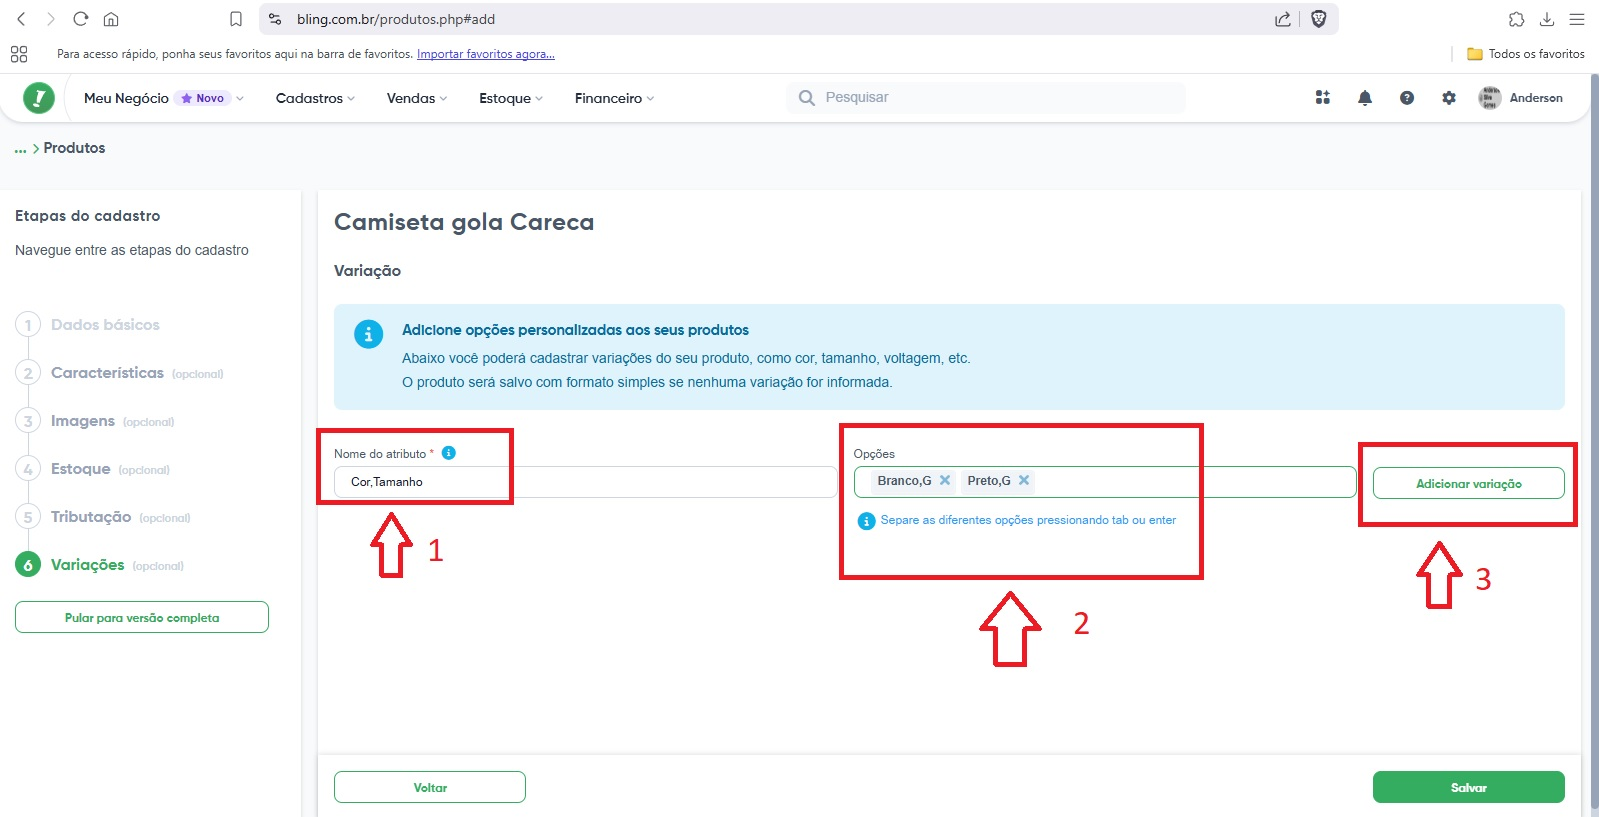
\includegraphics{images/np1/30-cadastro-produtos-variações-produto.jpg} 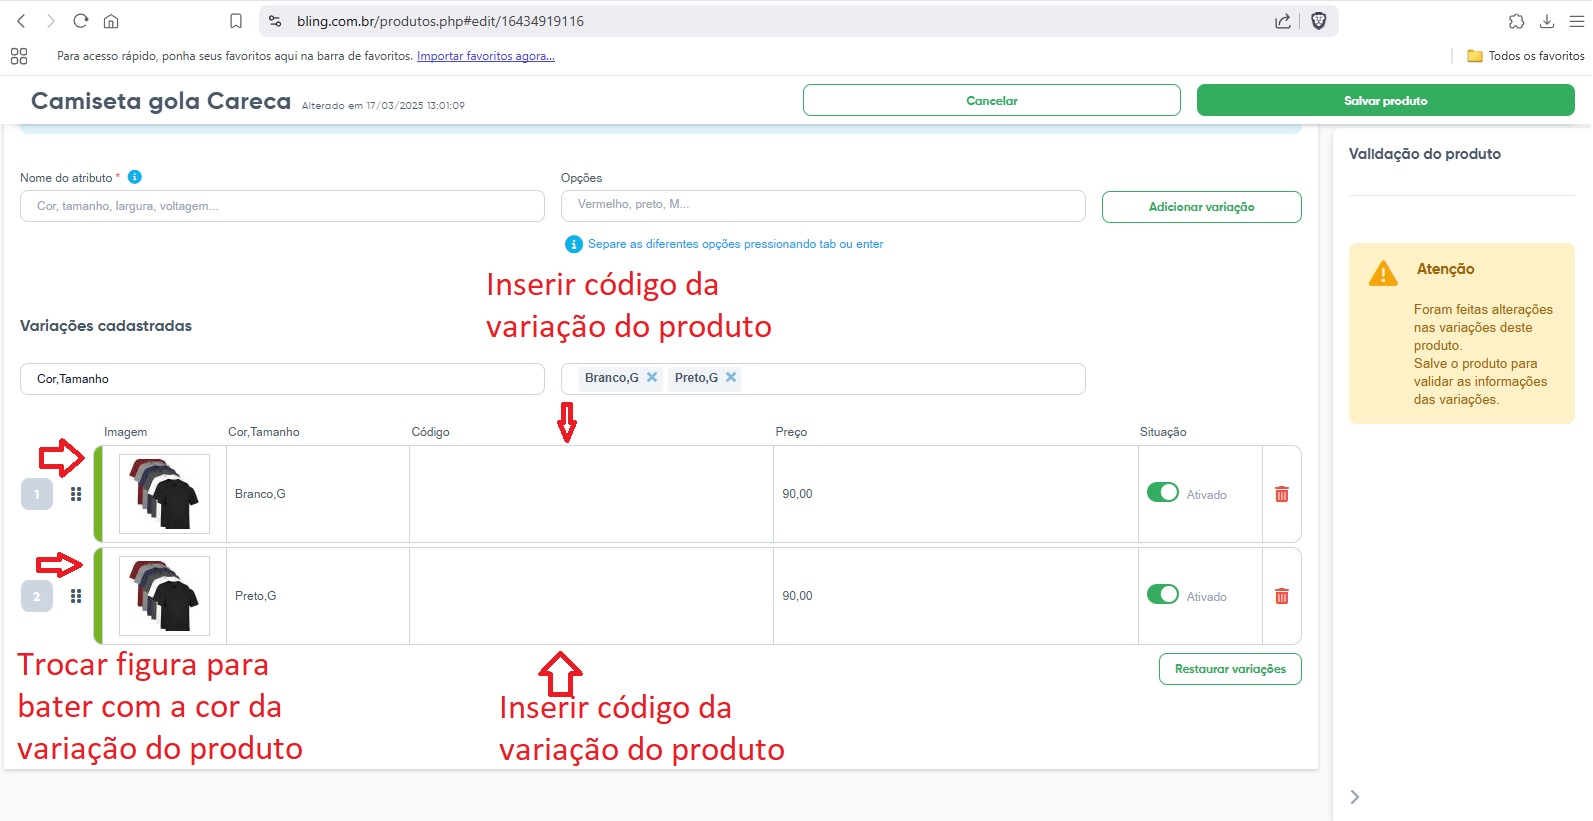
\includegraphics{images/np1/31-cadastro-produtos-variações-produto.jpg} 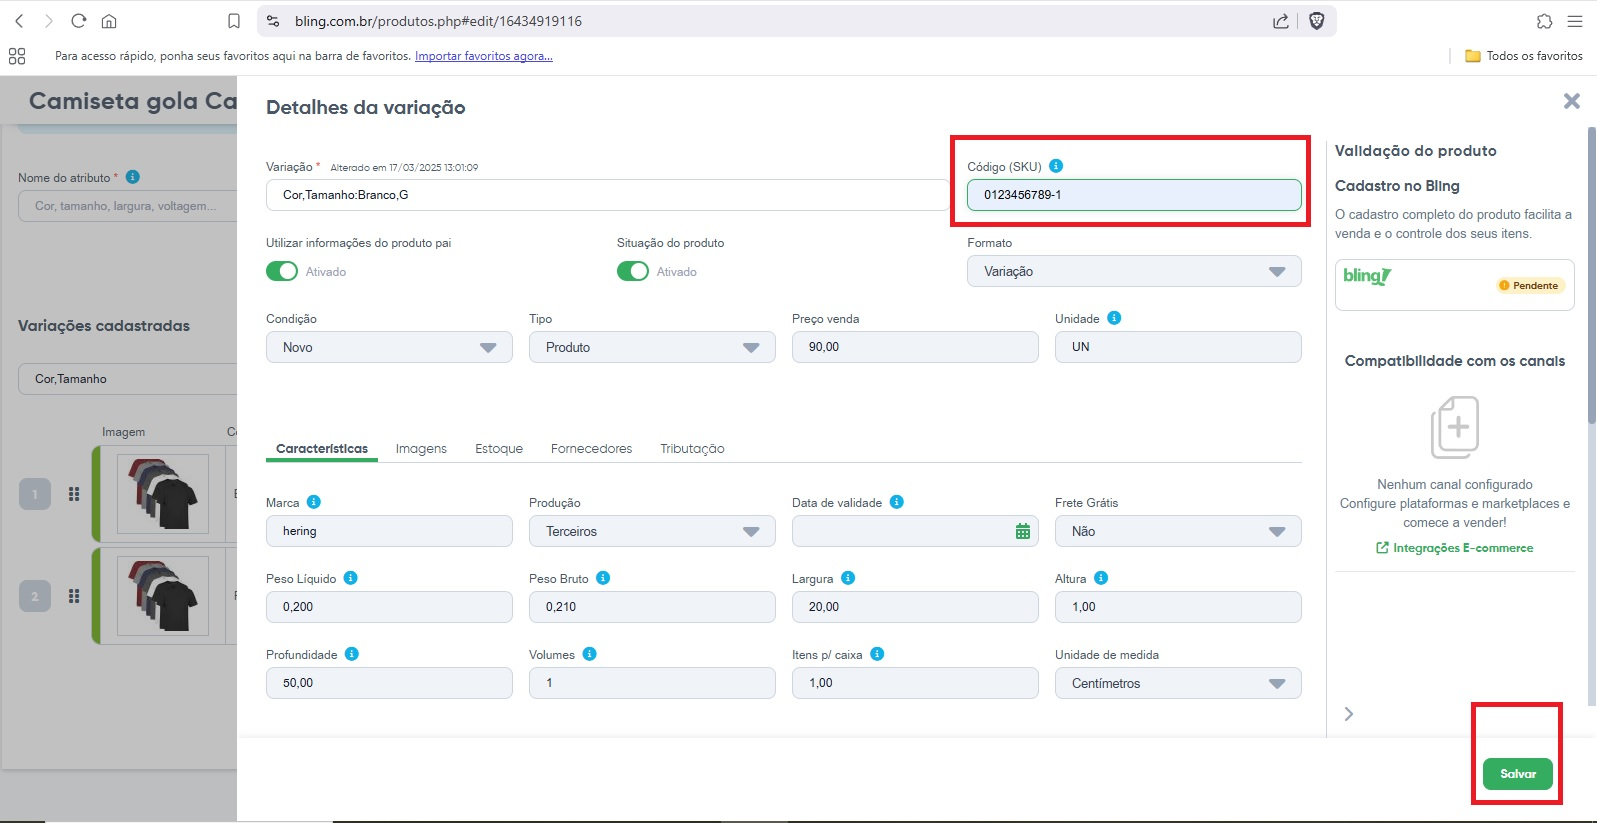
\includegraphics{images/np1/32-cadastro-produtos-variações-produto-inserir-código.jpg} 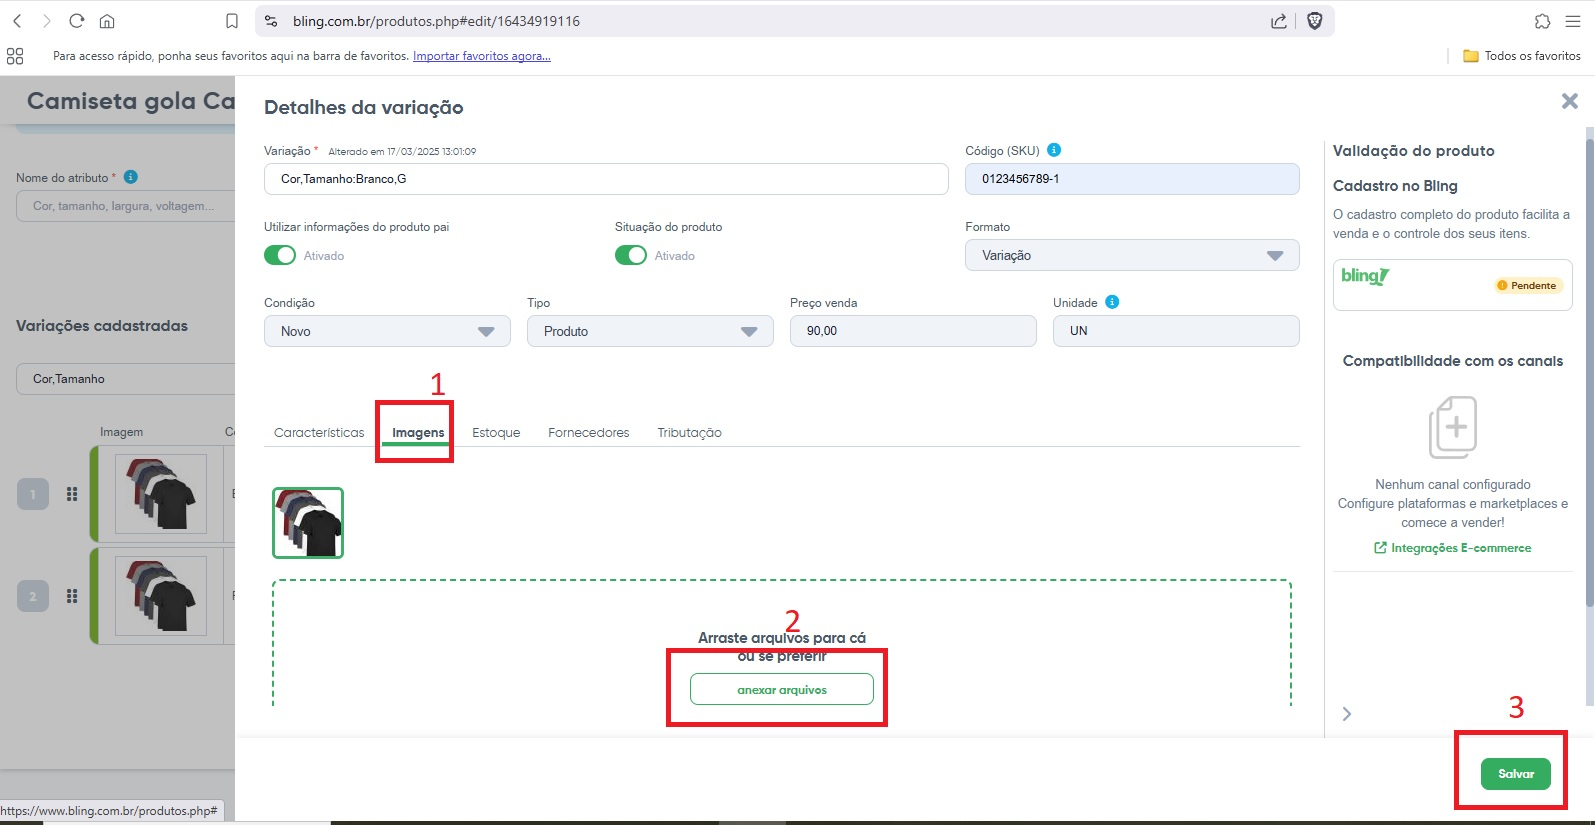
\includegraphics{images/np1/33-cadastro-produtos-variações-produto-inserir-imagem.jpg} \includegraphics{images/np1/34-cadastro-produtos-variações-produto.jpg}

\paragraph{Começar a cadastrar o estoque (Conceito de ``Módulo CONTROLE DE ESTOQUE'' dos ERPs)}\label{comeuxe7ar-a-cadastrar-o-estoque-conceito-de-muxf3dulo-controle-de-estoque-dos-erps}

\includegraphics{images/np1/35-bling-produto-cadastrado-sem-estoque.jpg} \includegraphics{images/np1/36-bling-estoque-produto-incluir.jpg} \includegraphics{images/np1/37-bling-estoque-produto-incluir-camiseta-preta.jpg} \includegraphics{images/np1/38-bling-estoque-produto-incluir-camiseta-preta-iniciar.jpg} \includegraphics{images/np1/39-bling-estoque-produto-incluir-camiseta-preta-feito.jpg} \includegraphics{images/np1/40-bling-estoque-produto-lançado.jpg} \includegraphics{images/np1/41-bling-cadastrar-cliente.jpg} \includegraphics{images/np1/42-bling-cadastrar-cliente-feito.jpg} \includegraphics{images/np1/43-bling-cadastrar-cliente-feito.jpg} \includegraphics{images/np1/44-bling-cadastrar-fornecedor-feito.jpg} \includegraphics{images/np1/45-bling-cadastrar-fornecedor-feito.jpg}

\subsubsection{Começar a cadastrar PDV (Ponto de Venda) da parte física da loja (Conceito de ``Módulo de vendas - PDV'' dos ERPs)}\label{comeuxe7ar-a-cadastrar-pdv-ponto-de-venda-da-parte-fuxedsica-da-loja-conceito-de-muxf3dulo-de-vendas---pdv-dos-erps}

\includegraphics{images/np1/46-bling-abrir-loja-fisica-frente-caixa.jpg} \includegraphics{images/np1/47-bling-abrir-loja-fisica-frente-caixa-ignorar-certificado.jpg} \includegraphics{images/np1/48-bling-abrir-loja-fisica-frente-caixa-cadastrar-loja-matriz.jpg} \includegraphics{images/np1/49-bling-abrir-loja-fisica-frente-caixa-cadastrar-loja-matriz.jpg} \includegraphics{images/np1/50-bling-abrir-loja-fisica-frente-caixa-ativo.jpg}

\subsection{Impantando o E-COMMERCE (parte virtual loja)}\label{impantando-o-e-commerce-parte-virtual-loja}

\subsection{ATIVE a PLATAFORMA DE E-COMMERCE}\label{ative-a-plataforma-de-e-commerce}

\subsubsection{cadastre a empresa do cliente na platafroma de e-commerce}\label{cadastre-a-empresa-do-cliente-na-platafroma-de-e-commerce}

\includegraphics{images/np1/51-nuvemshop-testar-loja-gratis.jpg} \includegraphics{images/np1/52-nuvemshop-cadastrar-loja-gratis.jpg} \includegraphics{images/np1/53-nuvemshop-testar-loja-gratis.jpg} \includegraphics{images/np1/54-nuvemshop-cadastrar-loja-gratis.jpg} \includegraphics{images/np1/55-nuvemshop-cadastrar-loja-gratis.jpg}

\subsubsection{cadastre as categorias de produtos na loja on-line}\label{cadastre-as-categorias-de-produtos-na-loja-on-line}

\includegraphics{images/np1/56-nuvemshop-cadastrar-categorias-produtos.jpg} \includegraphics{images/np1/57-nuvemshop-acessar-cadastro-categorias-produtos.jpg} \includegraphics{images/np1/58-nuvemshop-acessar-cadastro-categorias-produtos.jpg} \includegraphics{images/np1/59-nuvemshop-cadastrar-categorias-produtos.jpg} \includegraphics{images/np1/60-nuvemshop-cadastrar-subcategorias-produtos.jpg} \includegraphics{images/np1/61-nuvemshop-categorias-bling.jpg}

\subsubsection{mapeie o código das categorias de produtos na loja on-line para colocar no ERP depois}\label{mapeie-o-cuxf3digo-das-categorias-de-produtos-na-loja-on-line-para-colocar-no-erp-depois}

\includegraphics{images/np1/62-nuvemshop-obter-código-categorias.jpg} \includegraphics{images/np1/63-nuvemshop-obter-código-categorias.jpg} \includegraphics{images/np1/64-nuvemshop-categorias-nuvemshop-códigos.jpg} \includegraphics{images/np1/65-nuvemshop-visitar-loja-online.jpg} \includegraphics{images/np1/66-nuvemshop-visitar-loja-online.jpg} \includegraphics{images/np1/67-nuvemshop-visitar-loja-online.jpg}

\subsection{Inicie a amarração (integração) do e-commerce com o ERP (começando no e-commerce)}\label{inicie-a-amarrauxe7uxe3o-integrauxe7uxe3o-do-e-commerce-com-o-erp-comeuxe7ando-no-e-commerce}

\subsubsection{Instale o aplicativo (API) de conexão no e-commerce}\label{instale-o-aplicativo-api-de-conexuxe3o-no-e-commerce}

\includegraphics{images/np1/68-Conectar-nuvemshop-bling.jpg} \includegraphics{images/np1/69-Conectar-nuvemshop-bling.jpg} \includegraphics{images/np1/70-Conectar-nuvemshop-bling.jpg} \includegraphics{images/np1/71-Conectar-nuvemshop-bling.jpg}

\subsubsection{Instale o aplicativo (API) de conexão no ERP}\label{instale-o-aplicativo-api-de-conexuxe3o-no-erp}

\includegraphics{images/np1/72-Conectar-bling-nuvemshop.jpg} \includegraphics{images/np1/73-Conectar-bling-nuvemshop.jpg} \includegraphics{images/np1/74-Conectar-bling-nuvemshop-ajustes-finos.jpg} \includegraphics{images/np1/75-Conectar-bling-nuvemshop-ajustes-finos.jpg} \includegraphics{images/np1/76-Conectar-bling-nuvemshop-ajustes-finos-vendas.jpg} \includegraphics{images/np1/77-Conectar-bling-nuvemshop-ajustes-finos-vendas.jpg} \includegraphics{images/np1/78-Conectar-bling-nuvemshop-ajustes-feito.jpg}

\subsubsection{Faça agora o mapeamento do código das categorias do e-commerce no ERP}\label{fauxe7a-agora-o-mapeamento-do-cuxf3digo-das-categorias-do-e-commerce-no-erp}

\includegraphics{images/np1/79-Amarracao-Categorias-Ecommerce-ERP.jpg} \includegraphics{images/np1/80-Amarracao-Categorias-Ecommerce-ERP.jpg} \includegraphics{images/np1/81-Amarracao-Categorias-Ecommerce-ERP.jpg} \includegraphics{images/np1/82-Amarracao-Categorias-Ecommerce-ERP.jpg}

\subsubsection{Faça agora a exportação dos produtos}\label{fauxe7a-agora-a-exportauxe7uxe3o-dos-produtos}

\includegraphics{images/np1/83-Exportar-Bling-Nuvemshop.jpg} \includegraphics{images/np1/84-Exportar-Bling-Nuvemshop.jpg} \includegraphics{images/np1/85-Exportar-Bling-Nuvemshop.jpg} \includegraphics{images/np1/86-Exportar-Bling-Nuvemshop.jpg} \includegraphics{images/np1/87-Exportar-Bling-Nuvemshop.jpg} \includegraphics{images/np1/88-Exportar-Bling-Nuvemshop.jpg}

\subsubsection{Parabéns, hora de começar a testar seu e-commerce.}\label{parabuxe9ns-hora-de-comeuxe7ar-a-testar-seu-e-commerce.}

(lembre-se que vai faltar configurar o meio de pagamento no e-commerce para poder começar a receber)

\subsection{INICIANDO O PROCESSO DE VENDA SIMULADA NO E-COMMERCE INTEGRADO AO ERP:}\label{iniciando-o-processo-de-venda-simulada-no-e-commerce-integrado-ao-erp}

\chapter{INFRAESTRUTURA DE TIC}\label{infraestrutura-de-tic}

\section{Introdução:}\label{introduuxe7uxe3o-1}

\section{Componentes da Infraestrutura de TIC}\label{componentes-da-infraestrutura-de-tic}

\subsection{Hardware}\label{hardware}

\subsection{Redes de Computadores}\label{redes-de-computadores}

\subsection{Software}\label{software}

\subsubsection{Serviços de TIC}\label{serviuxe7os-de-tic}

\begin{longtable}[]{@{}
  >{\raggedright\arraybackslash}p{(\columnwidth - 4\tabcolsep) * \real{0.1391}}
  >{\raggedright\arraybackslash}p{(\columnwidth - 4\tabcolsep) * \real{0.7594}}
  >{\raggedright\arraybackslash}p{(\columnwidth - 4\tabcolsep) * \real{0.0986}}@{}}
\caption{Serviços de TIC}\tabularnewline
\toprule\noalign{}
\begin{minipage}[b]{\linewidth}\raggedright
Tipo de Serviço Corporativo
\end{minipage} & \begin{minipage}[b]{\linewidth}\raggedright
Descrição
\end{minipage} & \begin{minipage}[b]{\linewidth}\raggedright
Softwares servidores do serviço
\end{minipage} \\
\midrule\noalign{}
\endfirsthead
\toprule\noalign{}
\begin{minipage}[b]{\linewidth}\raggedright
Tipo de Serviço Corporativo
\end{minipage} & \begin{minipage}[b]{\linewidth}\raggedright
Descrição
\end{minipage} & \begin{minipage}[b]{\linewidth}\raggedright
Softwares servidores do serviço
\end{minipage} \\
\midrule\noalign{}
\endhead
\bottomrule\noalign{}
\endlastfoot
Correio eletrônico - E-Mail & Método de comunicação digital que permite o envio e recebimento de mensagens através da internet; & \begin{minipage}[t]{\linewidth}\raggedright
\begin{itemize}
\item
  Microsoft Exchage (windows)
\item
  Postfix (Linux)
\item
  Dovecot (Linux)
\item
  SMTPd (Linux)
\end{itemize}
\end{minipage} \\
Compartilhamento de Arquivos & Permite aos usuários armazenar, acessar e distribuir arquivos digitais pela internet; & \begin{minipage}[t]{\linewidth}\raggedright
\begin{itemize}
\item
  File Server (Windows)
\item
  SAMBA (Linux)
\item
  NFS (Linux)
\end{itemize}
\end{minipage} \\
Compartilhamento de Impressoras & Permite que vários computadores em uma rede corporativa utilizem uma única impressora; & \begin{minipage}[t]{\linewidth}\raggedright
\begin{itemize}
\item
  Spool Impressão (Windows)
\item
  CUPS (Linux)
\end{itemize}
\end{minipage} \\
Serviço de Nomes de Domínio - DNS & É essencialmente a ``lista telefônica'' da internet. Ele traduz nomes de domínio amigáveis (como ``\href{https://www.google.com/search?q=google.com}{google.com}'') em endereços IP numéricos (como ``172.217.160.142''), que os computadores usam para se comunicar entre si. & \begin{minipage}[t]{\linewidth}\raggedright
\begin{itemize}
\item
  Active Directory (Windows)
\item
  Bind (Linux)
\end{itemize}
\end{minipage} \\
Gerenciamento de usuários da rede corporativa & Um serviço de gerenciamento de usuários de rede corporativa, também conhecido como domínio, é um sistema centralizado que permite aos administradores de TI controlar e gerenciar o acesso de usuários e recursos em uma rede corporativa; & \begin{minipage}[t]{\linewidth}\raggedright
\begin{itemize}
\item
  Active Diretory (Windows)
\item
  LDAP (Linux)
\end{itemize}
\end{minipage} \\
\end{longtable}

\subsubsection{Sistemas de Gerenciamento de Banco de Dados}\label{sistemas-de-gerenciamento-de-banco-de-dados}

\section{Segurança em Sistemas de Informação}\label{seguranuxe7a-em-sistemas-de-informauxe7uxe3o}

\section{Exercícios de Fixação}\label{exercuxedcios-de-fixauxe7uxe3o}

\subsection{Hardware - Inventário}\label{hardware---inventuxe1rio}

\textbf{Exercício 1 -} Você precisa levantar o montante de capital para comprar equipamentos que vão informatizar a empresa com o seguinte layout.

A empresa tem 9 departamentos: Presidência com 3 funcionários, diretoria com 9 funcionários, departamento de TI 5 funcionários, departamento jurídico com 1 funcionário ,departamento de contabilidade com 5 funcionários, departamento de Recursos Humanos 3 funcionários, Departamento de Vendas 10 funcionários, Departamento de compras com 5 funcionários, Loja física com 10 funcionários e departamento de recursos materiais 5 funcionários. Com exceção dos funcionários da loja física, todos os funcionários usam um computador de mesa, uma mesa, um monitor 21 polegadas, uma cadeira e 1 telefone IP.

Baseado nestas informações, monte a distribuição de funcionários e equipamentos:

\begin{longtable}[]{@{}
  >{\raggedright\arraybackslash}p{(\columnwidth - 12\tabcolsep) * \real{0.1429}}
  >{\raggedright\arraybackslash}p{(\columnwidth - 12\tabcolsep) * \real{0.1429}}
  >{\raggedright\arraybackslash}p{(\columnwidth - 12\tabcolsep) * \real{0.1429}}
  >{\raggedright\arraybackslash}p{(\columnwidth - 12\tabcolsep) * \real{0.1429}}
  >{\raggedright\arraybackslash}p{(\columnwidth - 12\tabcolsep) * \real{0.1429}}
  >{\raggedright\arraybackslash}p{(\columnwidth - 12\tabcolsep) * \real{0.1429}}
  >{\raggedright\arraybackslash}p{(\columnwidth - 12\tabcolsep) * \real{0.1429}}@{}}
\caption{Tabela 1 - Funcionários e equipamentos por departamento}\tabularnewline
\toprule\noalign{}
\begin{minipage}[b]{\linewidth}\raggedright
Departamento
\end{minipage} & \begin{minipage}[b]{\linewidth}\raggedright
Funcionários
\end{minipage} & \begin{minipage}[b]{\linewidth}\raggedright
ComputadoresdeMesa
\end{minipage} & \begin{minipage}[b]{\linewidth}\raggedright
Mesas
\end{minipage} & \begin{minipage}[b]{\linewidth}\raggedright
Monitores21''
\end{minipage} & \begin{minipage}[b]{\linewidth}\raggedright
Cadeiras
\end{minipage} & \begin{minipage}[b]{\linewidth}\raggedright
TelefonesIP
\end{minipage} \\
\midrule\noalign{}
\endfirsthead
\toprule\noalign{}
\begin{minipage}[b]{\linewidth}\raggedright
Departamento
\end{minipage} & \begin{minipage}[b]{\linewidth}\raggedright
Funcionários
\end{minipage} & \begin{minipage}[b]{\linewidth}\raggedright
ComputadoresdeMesa
\end{minipage} & \begin{minipage}[b]{\linewidth}\raggedright
Mesas
\end{minipage} & \begin{minipage}[b]{\linewidth}\raggedright
Monitores21''
\end{minipage} & \begin{minipage}[b]{\linewidth}\raggedright
Cadeiras
\end{minipage} & \begin{minipage}[b]{\linewidth}\raggedright
TelefonesIP
\end{minipage} \\
\midrule\noalign{}
\endhead
\bottomrule\noalign{}
\endlastfoot
Presidência & 3 & 3 & 3 & 3 & 3 & 3 \\
Diretoria & 9 & 9 & 9 & 9 & 9 & 9 \\
DepartamentodeTI & 5 & 5 & 5 & 5 & 5 & 5 \\
DepartamentoJurídico & 1 & 1 & 1 & 1 & 1 & 1 \\
DepartamentodeContabilidade & 5 & 5 & 5 & 5 & 5 & 5 \\
DepartamentodeRH & 3 & 3 & 3 & 3 & 3 & 3 \\
DepartamentodeVendas & 10 & 10 & 10 & 10 & 10 & 10 \\
DepartamentodeCompras & 5 & 5 & 5 & 5 & 5 & 5 \\
LojaFísica & 10 & 0 & 0 & 0 & 0 & 0 \\
DepartamentodeRecursosMateriais & 5 & 5 & 5 & 5 & 5 & 5 \\
Total & 56 & 51 & 51 & 51 & 51 & 51 \\
\end{longtable}

Os equipamentos serão adquiridos em leilão. O melhor preço encontrado para cada item foi o seguinte:

\begin{enumerate}
\def\labelenumi{\arabic{enumi}.}
\item
  Computador de mesa : R\$ 4.289,00
\item
  Monitores 21' : R\$ 422,92
\item
  Mesas : R\$ 195,00
\item
  Cadeiras : R\$ 24,51
\item
  Telefones IP : R\$ 589,34
\end{enumerate}

Calcule:

\begin{enumerate}
\def\labelenumi{\alph{enumi})}
\item
  Qual o INVESTIMENTO de cada departamento com cada equipamento ?
\item
  Qual o INVESTIMENTO da empresa com cada classe de equipamento ?
\end{enumerate}

\begin{longtable}[]{@{}
  >{\raggedright\arraybackslash}p{(\columnwidth - 10\tabcolsep) * \real{0.1667}}
  >{\raggedright\arraybackslash}p{(\columnwidth - 10\tabcolsep) * \real{0.1667}}
  >{\raggedright\arraybackslash}p{(\columnwidth - 10\tabcolsep) * \real{0.1667}}
  >{\raggedright\arraybackslash}p{(\columnwidth - 10\tabcolsep) * \real{0.1667}}
  >{\raggedright\arraybackslash}p{(\columnwidth - 10\tabcolsep) * \real{0.1667}}
  >{\raggedright\arraybackslash}p{(\columnwidth - 10\tabcolsep) * \real{0.1667}}@{}}
\toprule\noalign{}
\begin{minipage}[b]{\linewidth}\raggedright
Departamento
\end{minipage} & \begin{minipage}[b]{\linewidth}\raggedright
Computadores
\end{minipage} & \begin{minipage}[b]{\linewidth}\raggedright
Monitores
\end{minipage} & \begin{minipage}[b]{\linewidth}\raggedright
Mesas
\end{minipage} & \begin{minipage}[b]{\linewidth}\raggedright
Cadeiras
\end{minipage} & \begin{minipage}[b]{\linewidth}\raggedright
TelefonesIP
\end{minipage} \\
\midrule\noalign{}
\endhead
\bottomrule\noalign{}
\endlastfoot
Presidência & R\$ 12.867,00 & R\$ 1.268,76 & R\$ 585,00 & R\$ 73,53 & R\$ 1.768,02 \\
Diretoria & R\$ 38.601,00 & R\$ 3.806,28 & R\$ 1.755,00 & R\$ 220,59 & R\$ 5.304,06 \\
DepartamentodeTI & R\$ 21.445,00 & R\$ 2.114,60 & R\$ 975,00 & R\$ 122,55 & R\$ 2.946,70 \\
DepartamentoJurídico & R\$ 4.289,00 & R\$ 422,92 & R\$ 195,00 & R\$ 24,51 & R\$ 589,34 \\
DepartamentodeContabilidade & R\$ 21.445,00 & R\$ 2.114,60 & R\$ 975,00 & R\$ 122,55 & R\$ 2.946,70 \\
DepartamentodeRH & R\$ 12.867,00 & R\$ 1.268,76 & R\$ 585,00 & R\$ 73,53 & R\$ 1.768,02 \\
DepartamentodeVendas & R\$ 42.890,00 & R\$ 4.229,20 & R\$ 1.950,00 & R\$ 245,10 & R\$ 5.893,40 \\
DepartamentodeCompras & R\$ 21.445,00 & R\$ 2.114,60 & R\$ 975,00 & R\$ 122,55 & R\$ 2.946,70 \\
LojaFísica & R\$ 0,00 & R\$ 0,00 & R\$ 0,00 & R\$ 0,00 & R\$ 0,00 \\
DepartamentodeRecursosMateriais & R\$ 21.445,00 & R\$ 2.114,60 & R\$ 975,00 & R\$ 122,55 & R\$ 2.946,70 \\
TotalGeral & R\$ 218.739,00 & R\$ 21.146,00 & R\$ 9.750,00 & R\$ 1.225,50 & R\$ 29.467,00 \\
\end{longtable}

\begin{enumerate}
\def\labelenumi{\alph{enumi})}
\setcounter{enumi}{1}
\item
  Qual o INVESTIMENTO de cada departamento com TIC ?
\item
  Qual o INVESTIMENTO necessário em TIC para informatizar a empresa ?
\end{enumerate}

\begin{longtable}[]{@{}
  >{\raggedright\arraybackslash}p{(\columnwidth - 4\tabcolsep) * \real{0.3333}}
  >{\raggedright\arraybackslash}p{(\columnwidth - 4\tabcolsep) * \real{0.3333}}
  >{\raggedright\arraybackslash}p{(\columnwidth - 4\tabcolsep) * \real{0.3333}}@{}}
\toprule\noalign{}
\begin{minipage}[b]{\linewidth}\raggedright
Departamento
\end{minipage} & \begin{minipage}[b]{\linewidth}\raggedright
Custo total TIC Por departamento R\$
\end{minipage} & \begin{minipage}[b]{\linewidth}\raggedright
Custo total de TIC da empresa R\$
\end{minipage} \\
\midrule\noalign{}
\endhead
\bottomrule\noalign{}
\endlastfoot
Presidência & R\$ 16.562,31 & R\$ 280.328,50 \\
Diretoria & R\$ 49.686,93 & \\
Departamentode TI & R\$ 27.603,85 & \\
Departamento Jurídico & R\$ 5.520,77 & \\
Departamentode Contabilidade & R\$ 27.603,85 & \\
Departamentode RH & R\$ 16.562,31 & \\
Departamentode Vendas & R\$ 55.207,70 & \\
Departamentode Compras & R\$ 27.603,85 & \\
Loja Física & R\$ 0,00 & \\
Departamento de Recursos Materiais & R\$ 27.603,85 & \\
\end{longtable}

\chapter{SISTEMAS DE INFORMAÇÃO E FUNCIONALIDADES}\label{sistemas-de-informauxe7uxe3o-e-funcionalidades}

\section{Sistemas Integrados de Gestão}\label{sistemas-integrados-de-gestuxe3o}

\section{Comércio Eletrônico}\label{comuxe9rcio-eletruxf4nico}

\chapter{Tomada de Decisão de Gestão do Conhecimento: Business Inteligence}\label{tomada-de-decisuxe3o-de-gestuxe3o-do-conhecimento-business-inteligence}

\section{Ferramentas de B.I. e conceito de DashBoard}\label{ferramentas-de-b.i.-e-conceito-de-dashboard}

\subsection{PowerBI}\label{powerbi}

\section{Bancos de Dados OLTP e OLAP}\label{bancos-de-dados-oltp-e-olap}

\chapter{TECNOLOGIAS EMERGENTES E INOVAÇÃO EM TIC}\label{tecnologias-emergentes-e-inovauxe7uxe3o-em-tic}

\section{VIRTUALIZAÇÃO E CONTINENTIZAÇÃO}\label{virtualizauxe7uxe3o-e-continentizauxe7uxe3o}

\section{BIG DATA}\label{big-data}

\section{ASSISTENTES INTELIGENTES}\label{assistentes-inteligentes}

\chapter{GESTÃO DO CONHECIMENTO EM TIC}\label{gestuxe3o-do-conhecimento-em-tic}

\section{Conceitos e Práticas de Gestão do Conhecimento}\label{conceitos-e-pruxe1ticas-de-gestuxe3o-do-conhecimento}

\section{Implementação e Desafios da Gestão do Conhecimento}\label{implementauxe7uxe3o-e-desafios-da-gestuxe3o-do-conhecimento}

\chapter{APLICATIVOS DE PRODUTIVIDADE E ESCRITÓRIO I}\label{aplicativos-de-produtividade-e-escrituxf3rio-i}

\section{Planilhas Eletrônicas}\label{planilhas-eletruxf4nicas}

\section{Processadores de Texto}\label{processadores-de-texto}

\chapter{APLICATIVOS DE PRODUTIVIDADE E ESCRITÓRIO II}\label{aplicativos-de-produtividade-e-escrituxf3rio-ii}

\section{Ferramentas de Apresentação}\label{ferramentas-de-apresentauxe7uxe3o}

\section{Tecnologias de Comunicação e Colaboração}\label{tecnologias-de-comunicauxe7uxe3o-e-colaborauxe7uxe3o}

  \bibliography{book.bib,packages.bib}

\end{document}
